% main_v2.tex — Master document (Technical Report, v2.0)
% Video-to-Gaussian: An Agentic Pipeline for Volumetric Cultural
% Heritage Preservation with Hierarchical Scene Reconstruction
%
% Dr John O'Hare, DreamLab AI Consulting Ltd
% For: Roger McKinley, University of Salford
% June 2026
%
% Supersedes v1.0. Technically-focused. Not confidential.

\documentclass[a4paper,11pt,twoside,openright]{report}

% ────────────────────────────────────────────────────────────
% Language and encoding
% ────────────────────────────────────────────────────────────
\usepackage[utf8]{inputenc}
\usepackage[T1]{fontenc}
\usepackage[british]{babel}
\usepackage{microtype}

% ────────────────────────────────────────────────────────────
% Page geometry
% ────────────────────────────────────────────────────────────
\usepackage[
  a4paper,
  top=30mm,
  bottom=30mm,
  inner=30mm,
  outer=25mm,
  headheight=14pt
]{geometry}

% ────────────────────────────────────────────────────────────
% Fonts
% ────────────────────────────────────────────────────────────
\usepackage{lmodern}
\usepackage{inconsolata}

% ────────────────────────────────────────────────────────────
% Colours
% ────────────────────────────────────────────────────────────
\usepackage[dvipsnames,svgnames,x11names]{xcolor}

\definecolor{UoSRed}{HTML}{B71234}
\definecolor{DreamLabAccent}{HTML}{6366F1}
\definecolor{DarkBg}{HTML}{0F172A}
\definecolor{MidGrey}{HTML}{64748B}
\definecolor{LightGrey}{HTML}{F1F5F9}
\definecolor{CodeBg}{HTML}{1E293B}
\definecolor{SuccessGreen}{HTML}{22C55E}
\definecolor{WarningAmber}{HTML}{F59E0B}

% ────────────────────────────────────────────────────────────
% Graphics and figures
% ────────────────────────────────────────────────────────────
\usepackage{graphicx}
\graphicspath{{figures/}{diagrams/}}
\usepackage{subcaption}
\usepackage{float}
\usepackage{wrapfig}

% ────────────────────────────────────────────────────────────
% TikZ and pgfplots
% ────────────────────────────────────────────────────────────
\usepackage{tikz}
\usetikzlibrary{
  calc,
  positioning,
  arrows.meta,
  shapes.geometric,
  decorations.markings,
  backgrounds,
  fit,
  patterns,
  shadows,
  fadings
}
\usepackage{pgfplots}
\pgfplotsset{compat=1.18}

% ────────────────────────────────────────────────────────────
% Tables
% ────────────────────────────────────────────────────────────
\usepackage{booktabs}
\usepackage{tabularx}
\usepackage{longtable}
\usepackage{multirow}
\usepackage{array}
\newcolumntype{L}[1]{>{\raggedright\arraybackslash}p{#1}}
\newcolumntype{C}[1]{>{\centering\arraybackslash}p{#1}}
\newcolumntype{R}[1]{>{\raggedleft\arraybackslash}p{#1}}

% ────────────────────────────────────────────────────────────
% Bibliography
% ────────────────────────────────────────────────────────────
\usepackage[
  backend=biber,
  style=authoryear-comp,
  natbib=true,
  sorting=nyt,
  maxbibnames=99,
  maxcitenames=2,
  giveninits=true,
  uniquename=init,
  url=true,
  doi=true,
  isbn=false,
  eprint=false
]{biblatex}
\addbibresource{references.bib}

% ────────────────────────────────────────────────────────────
% Hyperlinks
% ────────────────────────────────────────────────────────────
\usepackage[
  colorlinks=true,
  linkcolor=UoSRed,
  citecolor=DreamLabAccent,
  urlcolor=DreamLabAccent,
  bookmarks=true,
  bookmarksnumbered=true,
  pdfauthor={Dr John O'Hare},
  pdftitle={Video-to-Gaussian: An Agentic Pipeline for Volumetric Cultural Heritage Preservation},
  pdfsubject={3D Gaussian Splatting, Hierarchical Scene Reconstruction, Cultural Heritage},
  pdfkeywords={Gaussian Splatting, Scene Graph, SAM2, Generative Reconstruction, USD, Cultural Heritage}
]{hyperref}
\usepackage{bookmark}

% ────────────────────────────────────────────────────────────
% Headers and footers
% ────────────────────────────────────────────────────────────
\usepackage{fancyhdr}

\pagestyle{fancy}
\fancyhf{}
\fancyhead[LE]{\small\textcolor{MidGrey}{\leftmark}}
\fancyhead[RO]{\small\textcolor{MidGrey}{\rightmark}}
\fancyfoot[LE,RO]{\small\textcolor{MidGrey}{\thepage}}
\fancyfoot[CE,CO]{\small\textcolor{MidGrey}{DreamLab AI Consulting Ltd}}
\renewcommand{\headrulewidth}{0.4pt}
\renewcommand{\footrulewidth}{0.2pt}
\renewcommand{\headrule}{\hbox to\headwidth{\color{UoSRed}\leaders\hrule height \headrulewidth\hfill}}
\renewcommand{\footrule}{\hbox to\headwidth{\color{LightGrey}\leaders\hrule height \footrulewidth\hfill}}

\fancypagestyle{plain}{%
  \fancyhf{}
  \fancyfoot[LE,RO]{\small\textcolor{MidGrey}{\thepage}}
  \renewcommand{\headrulewidth}{0pt}
  \renewcommand{\footrulewidth}{0.2pt}
}

% ────────────────────────────────────────────────────────────
% Code listings
% ────────────────────────────────────────────────────────────
\usepackage{listings}
\lstset{
  basicstyle=\ttfamily\small,
  backgroundcolor=\color{LightGrey},
  frame=single,
  rulecolor=\color{MidGrey},
  breaklines=true,
  breakatwhitespace=true,
  showstringspaces=false,
  tabsize=2,
  captionpos=b,
  numbers=left,
  numberstyle=\tiny\color{MidGrey},
  keywordstyle=\color{DreamLabAccent}\bfseries,
  commentstyle=\color{MidGrey}\itshape,
  stringstyle=\color{SuccessGreen}
}

% ────────────────────────────────────────────────────────────
% Coloured boxes (tcolorbox)
% ────────────────────────────────────────────────────────────
\usepackage[most]{tcolorbox}

% Key Finding box
\newtcolorbox{keyfinding}[1][]{%
  enhanced,
  colback=UoSRed!5,
  colframe=UoSRed,
  fonttitle=\bfseries,
  title={Key Finding},
  left=6mm,
  sharp corners=south,
  boxrule=0.8pt,
  toptitle=2mm,
  bottomtitle=2mm,
  attach boxed title to top left={xshift=10mm, yshift=-\tcboxedtitleheight/2},
  boxed title style={
    colback=UoSRed,
    colframe=UoSRed,
    sharp corners,
    size=small
  },
  #1
}

% Recommendation box
\newtcolorbox{recommendation}[1][]{%
  enhanced,
  colback=DreamLabAccent!5,
  colframe=DreamLabAccent,
  fonttitle=\bfseries,
  title={Recommendation},
  left=6mm,
  sharp corners=south,
  boxrule=0.8pt,
  toptitle=2mm,
  bottomtitle=2mm,
  attach boxed title to top left={xshift=10mm, yshift=-\tcboxedtitleheight/2},
  boxed title style={
    colback=DreamLabAccent,
    colframe=DreamLabAccent,
    sharp corners,
    size=small
  },
  #1
}

% Technical Note box
\newtcolorbox{technote}[1][]{%
  enhanced,
  colback=CodeBg!5,
  colframe=MidGrey,
  fonttitle=\bfseries\color{white},
  title={Technical Note},
  left=6mm,
  boxrule=0.6pt,
  toptitle=2mm,
  bottomtitle=2mm,
  attach boxed title to top left={xshift=10mm, yshift=-\tcboxedtitleheight/2},
  boxed title style={
    colback=MidGrey,
    colframe=MidGrey,
    sharp corners,
    size=small
  },
  #1
}

% ────────────────────────────────────────────────────────────
% Glossaries and index
% ────────────────────────────────────────────────────────────
\usepackage[acronym,toc,nonumberlist]{glossaries}
\makeglossaries

\newacronym{3dgs}{3DGS}{3D Gaussian Splatting}
\newacronym{sfm}{SfM}{Structure from Motion}
\newacronym{mvs}{MVS}{Multi-View Stereo}
\newacronym{tsdf}{TSDF}{Truncated Signed Distance Function}
\newacronym{ich}{ICH}{Intangible Cultural Heritage}
\newacronym{uos}{UoS}{University of Salford}
\newacronym{sam}{SAM}{Segment Anything Model}
\newacronym{nerf}{NeRF}{Neural Radiance Fields}
\newacronym{mrnf}{MRNF}{Mini-Splatting with Relocation and Normal Filtering}
\newacronym{mcmc}{MCMC}{Markov Chain Monte Carlo}
\newacronym{usd}{USD}{Universal Scene Description}
\newacronym{webgl}{WebGL}{Web Graphics Library}
\newacronym{webgpu}{WebGPU}{Web Graphics Processing Unit API}
\newacronym{colmap}{COLMAP}{COLlaborative MAPping}
\newacronym{ke}{KE}{Knowledge Exchange}
\newacronym{cop}{CoP}{Community of Practice}
\newacronym{gpu}{GPU}{Graphics Processing Unit}
\newacronym{mcp}{MCP}{Model Context Protocol}
\newacronym{psnr}{PSNR}{Peak Signal-to-Noise Ratio}
\newacronym{ssim}{SSIM}{Structural Similarity Index Measure}
\newacronym{lpips}{LPIPS}{Learned Perceptual Image Patch Similarity}
\newacronym{come}{CoMe}{Confidence-based Meshing}
\newacronym{gw}{GW}{Gaussian Wrapping}
\newacronym{milo}{MILo}{Mesh-In-the-Loop Gaussian Splatting}
\newacronym{pbr}{PBR}{Physically-Based Rendering}
\newacronym{abi}{ABI}{Application Binary Interface}
\newacronym{cpu}{CPU}{Central Processing Unit}
\newacronym{llm}{LLM}{Large Language Model}
\newacronym{ui}{UI}{User Interface}
\newacronym{vr}{VR}{Virtual Reality}
\newacronym{vram}{VRAM}{Video Random-Access Memory}
\newacronym{adr}{ADR}{Architecture Decision Record}
\newacronym{ddd}{DDD}{Domain-Driven Design}
\newacronym{gsg}{GSG}{Gaussian Scene Graph}
\newacronym{ksplat}{KSPLAT}{Compressed Gaussian Splat container}

\usepackage{makeidx}
\makeindex

% ────────────────────────────────────────────────────────────
% Miscellaneous
% ────────────────────────────────────────────────────────────
\usepackage{enumitem}
\setlist{nosep,leftmargin=*}
\usepackage{pdfpages}
\usepackage{csquotes}
\usepackage{siunitx}
\usepackage{amsmath,amssymb}
\usepackage{etoolbox}

% Chapter title formatting
\usepackage{titlesec}
\titleformat{\chapter}[display]
  {\normalfont\huge\bfseries\color{DarkBg}}
  {\textcolor{UoSRed}{\chaptertitlename\ \thechapter}}{10pt}{\Huge}
\titlespacing*{\chapter}{0pt}{-20pt}{30pt}

\titleformat{\section}
  {\normalfont\Large\bfseries\color{DarkBg}}
  {\textcolor{UoSRed}{\thesection}}{1em}{}

\titleformat{\subsection}
  {\normalfont\large\bfseries\color{DarkBg}}
  {\textcolor{DreamLabAccent}{\thesubsection}}{1em}{}

\titleformat{\part}[display]
  {\centering\normalfont\Huge\bfseries\color{DarkBg}}
  {\textcolor{UoSRed}{\partname\ \thepart}}{10pt}{\huge}
\titlespacing*{\part}{0pt}{50pt}{40pt}

% ────────────────────────────────────────────────────────────
% Document metadata
% ────────────────────────────────────────────────────────────
\title{Video-to-Gaussian: An Agentic Pipeline for Volumetric Cultural Heritage Preservation}
\author{Dr John O'Hare \\ DreamLab AI Consulting Ltd}
\date{June 2026}

% ════════════════════════════════════════════════════════════
\begin{document}

% ────────────────────────────────────────────────────────────
% Title page
% ────────────────────────────────────────────────────────────
\begin{titlepage}
\begin{tikzpicture}[remember picture, overlay]
  % Full-bleed dark background
  \fill[DarkBg] (current page.south west) rectangle (current page.north east);

  % Geometric accent — radial dots
  \foreach \i in {1,...,60} {
    \pgfmathsetmacro{\xr}{rand*10}
    \pgfmathsetmacro{\yr}{rand*14}
    \pgfmathsetmacro{\op}{0.03 + rand*0.08}
    \fill[white, opacity=\op]
      ($(current page.south west) + (\xr,\yr)$) circle (1pt);
  }

  % Top-left geometric pattern — overlapping circles
  \foreach \r in {2,3.2,4.4,5.6} {
    \draw[UoSRed, opacity=0.15, line width=0.6pt]
      ($(current page.north west) + (2.5,-3)$) circle (\r);
  }

  % Bottom-right geometric pattern — diagonal lines
  \foreach \i in {0,0.8,...,6.4} {
    \draw[DreamLabAccent, opacity=0.10, line width=0.5pt]
      ($(current page.south east) + (-\i-1, 0.5)$) --
      ($(current page.south east) + (-0.5, \i+1)$);
  }

  % Horizontal accent bar
  \fill[UoSRed] ($(current page.west) + (0,2)$) rectangle ($(current page.east) + (0,2.08)$);
  \fill[DreamLabAccent] ($(current page.west) + (0,1.9)$) rectangle ($(current page.east) + (0,1.94)$);

  % Report type label
  \node[anchor=north west, text=UoSRed, font=\footnotesize\sffamily\bfseries, text width=13cm]
    at ($(current page.north west) + (3,-2)$)
    {TECHNICAL REPORT \textcolor{MidGrey}{|} AI \& KNOWLEDGE EXCHANGE \textcolor{MidGrey}{|} SYSTEM ARCHITECTURE \& RESULTS};

  % Main title
  \node[anchor=west, text=white, font=\fontsize{30}{34}\selectfont\bfseries\sffamily, text width=15cm]
    at ($(current page.west) + (3,5.5)$)
    {Video-to-Gaussian\\[6pt]};

  % Subtitle / tagline
  \node[anchor=west, text=white, font=\fontsize{16}{20}\selectfont\sffamily, text width=14cm]
    at ($(current page.west) + (3,2.6)$)
    {An Agentic Pipeline for Volumetric\\
     Cultural Heritage Preservation with\\
     Hierarchical Scene Reconstruction};

  % Technical descriptor
  \node[anchor=west, text=MidGrey, font=\normalsize\sffamily, text width=13cm]
    at ($(current page.west) + (3,-0.3)$)
    {3D Gaussian Splatting \textbullet\ SAM2 Segmentation \textbullet\ Generative\\
     Per-Object Reconstruction \textbullet\ USD Scene Graphs \textbullet\ Browser Delivery};

  % Author block
  \node[anchor=west, text=white, font=\sffamily, text width=10cm]
    at ($(current page.west) + (3,-2.6)$)
    {\textbf{Dr John O'Hare}\\[2pt]
     DreamLab AI Consulting Ltd\\[8pt]
     \textcolor{MidGrey}{Prepared for}\\[2pt]
     \textbf{Roger McKinley}\\[2pt]
     Creative Technology and Content Manager\\
     University of Salford};

  % Date
  \node[anchor=west, text=DreamLabAccent, font=\sffamily\bfseries]
    at ($(current page.west) + (3,-5.3)$)
    {June 2026};

  % Logo placeholders
  \node[anchor=south west, opacity=0.9]
    at ($(current page.south west) + (3,2)$)
    {\textcolor{white}{\sffamily\small [DreamLab AI Logo]}};

  \node[anchor=south east, opacity=0.9]
    at ($(current page.south east) + (-3,2)$)
    {\textcolor{white}{\sffamily\small [University of Salford Logo]}};

  % Version indicator
  \node[anchor=south east, text=MidGrey, font=\tiny\sffamily]
    at ($(current page.south east) + (-3,1)$)
    {v2.0 \textcolor{MidGrey}{|} TECHNICAL REPORT \textcolor{MidGrey}{|} SUPERSEDES v1.0};

\end{tikzpicture}
\end{titlepage}

% ────────────────────────────────────────────────────────────
% Front matter
% ────────────────────────────────────────────────────────────
\pagenumbering{roman}

% Executive summary
\chapter*{Executive Summary}
\addcontentsline{toc}{chapter}{Executive Summary}
\markboth{Executive Summary}{Executive Summary}

This report documents the architecture, implementation, and validated results of the \texttt{gaussian-toolkit}: an end-to-end, AI-orchestrated pipeline that transforms a single hand-held video walkthrough into a hierarchically-structured, editable, volumetric reconstruction of a cultural heritage space. It supersedes the v1.0 pilot report, reflecting a substantial uplift in the system's capability following its re-platforming onto LichtFeld~Studio~v0.5.2 and the completion of the scene-decomposition and generative-reconstruction subsystems.

Where the v1.0 pilot established that 3D Gaussian Splatting (\acrshort{3dgs}) was a \emph{viable} preservation medium, this report demonstrates a complete realisation of the project's original design goals. From a single 4K video capture, the pipeline now produces: (i)~a photorealistic Gaussian splat scene; (ii)~a watertight polygonal mesh of the environment via four pluggable extraction backends; (iii)~automatic, 3D-consistent decomposition of the scene into individually-addressable objects using \acrshort{sam}2; (iv)~independent, generatively-completed, textured polygonal meshes for each salient object, reconstructed in full 360\textdegree\ via a multi-view diffusion engine driven through ComfyUI; and (v)~a single hierarchical Universal Scene Description (\acrshort{usd}) scene graph in which every reconstructed object is emplaced at its surveyed position within the meshed environment.

The architectural centrepiece of the v2.0 system is the \textbf{splat-and-mesh dual representation governed by a single scene graph}. Rather than treating mesh extraction as a lossy terminal step, the pipeline maintains the Gaussian splat and the polygonal mesh as co-registered \acrshort{usd} variants of the same prims. A curator may view the scene as a photoreal splat in a browser, or as a game-engine-ready mesh hierarchy in Unreal Engine, with object-level selection, metadata association, and re-composition available in both. This resolves the central tension identified in the v1.0 report---that splat fidelity and mesh editability were mutually exclusive---by delivering both from one capture, bound together by surveyed geometry.

This report details the three-container compute architecture, the eight-stage processing pipeline, the integration of LichtFeld~Studio's native scene-graph harmonisation and \acrshort{mcp} control surface, the four mesh-extraction backends and their measured trade-offs, the per-object generative reconstruction subsystem, and the browser- and engine-based delivery mechanisms. It closes with a deployment roadmap for the University of Salford.

\tableofcontents
\listoffigures
\listoftables

% Print glossary in front matter
\printglossary[type=\acronymtype, title={Acronyms and Abbreviations}]

% ────────────────────────────────────────────────────────────
% Main matter
% ────────────────────────────────────────────────────────────
\cleardoublepage
\pagenumbering{arabic}

% ════════════════════════════════════════════════════════════
% Part I: System Architecture
% ════════════════════════════════════════════════════════════
\part{System Architecture}
\label{part:architecture}

\chapter{Introduction}
\label{ch:intro}

\section{From Pilot to Production}
\label{sec:intro-pilot}

The v1.0 report of this project established a hypothesis: that 3D Gaussian Splatting (\acrshort{3dgs}) could serve as a practical medium for preserving the spatial and experiential qualities of cultural heritage spaces that conventional photography and video cannot capture. That report demonstrated viability. It produced a photorealistic splat from a video walkthrough, observed that mesh extraction degraded fidelity, and recommended that splats be treated as preservation artefacts in their own right.

This report supersedes that pilot. In the intervening period the system was re-platformed onto LichtFeld~Studio~v0.5.2 \parencite{LichtFeldStudio2026}, and the segmentation, generative-reconstruction, and scene-assembly subsystems that the v1.0 report described as future work were completed and integrated. The \texttt{gaussian-toolkit} now realises the project's original design goals in full. From a single hand-held 4K video of a gallery interior, the pipeline produces not merely a splat, but a \emph{structured, editable, hierarchical reconstruction}: a photoreal Gaussian field, a watertight polygonal mesh of the environment, an automatic decomposition of the scene into individually-addressable objects, an independently reconstructed and fully-textured 360\textdegree\ mesh for each of those objects, and a single Universal Scene Description (\acrshort{usd}) scene graph that places every reconstructed object at its surveyed position within the meshed room.

\begin{keyfinding}
The v2.0 system resolves the central tension of the v1.0 pilot---that splat fidelity and mesh editability were mutually exclusive. It maintains the Gaussian splat and the polygonal mesh as co-registered variants of the same scene-graph prims. One capture yields both a photoreal browser experience and a game-engine-ready mesh hierarchy, bound together by surveyed geometry.
\end{keyfinding}

\section{The Preservation Problem}
\label{sec:intro-problem}

Immersive and experiential cultural works---installation art, site-specific performance, interactive exhibitions---resist conventional documentation. Their meaning is inseparable from the act of inhabiting them: the spatial relationships between objects, the way light falls across a room, the sequence in which a visitor encounters a work. A photograph flattens this; a video fixes a single path through it. Neither preserves the \emph{navigable space} itself \parencite{UNESCO2003,Champion2011}.

Volumetric reconstruction offers a different proposition: capture the space as a navigable three-dimensional field, from which any viewpoint can be synthesised after the fact. The challenge has historically been one of cost and expertise---laser scanning and photogrammetry demand specialist equipment, controlled conditions, and skilled operators \parencite{Remondino2011,Stylianidis2016}. The contribution of this project is to collapse that barrier: a single uncalibrated video, captured on a consumer phone, processed by an automated pipeline, yielding a result that is simultaneously archival-grade and audience-ready.

\section{Design Goals and Their Achievement}
\label{sec:intro-goals}

The project was funded by the University of Salford to trial whether contemporary AI reconstruction could meet a specific set of capability goals. Table~\ref{tab:intro-goals} states each goal as originally framed and the v2.0 outcome against it.

\begin{table}[htbp]
  \centering
  \caption{Stated design goals and their realisation in v2.0.}
  \label{tab:intro-goals}
  \begin{tabularx}{\textwidth}{@{}L{5.4cm}X@{}}
    \toprule
    \textbf{Design goal} & \textbf{v2.0 outcome} \\
    \midrule
    Photoreal capture of a heritage interior from consumer video &
    Achieved. A 4K phone walkthrough yields a 1.18M-Gaussian field at \acrshort{psnr}~29.6~dB in $\sim$24~minutes of \acrshort{gpu} time (Chapter~\ref{ch:reconstruction}). \\
    \addlinespace
    A polygonal mesh of the environment with a hierarchical scene graph &
    Achieved. Four pluggable backends extract the room mesh (Chapter~\ref{ch:meshing}); the \acrshort{usd} scene graph organises the result hierarchically (Chapter~\ref{ch:scenegraph}). \\
    \addlinespace
    Separate, 360\textdegree-reconstructed objects within the scene &
    Achieved. Salient objects are reconstructed independently as watertight, textured meshes via multi-view generative inference (Chapter~\ref{ch:scenegraph}). \\
    \addlinespace
    Objects extracted automatically by segmentation &
    Achieved. \acrshort{sam}2 decomposes the scene into 31 coherent object clusters with 98.3\% Gaussian coverage (Chapter~\ref{ch:scenegraph}). \\
    \addlinespace
    Objects turned into textured polygonal meshes by a generative engine &
    Achieved. Per-object orbit renders drive Hunyuan3D~2.0 through ComfyUI, with FLUX.1 background completion, yielding \acrshort{pbr}-textured meshes (Chapter~\ref{ch:scenegraph}). \\
    \addlinespace
    Emplacement of objects into the polygonal reconstruction &
    Achieved. Each object mesh is positioned at its \acrshort{colmap}-surveyed centroid within the environment mesh, in one scene graph (Chapter~\ref{ch:scenegraph}). \\
    \bottomrule
  \end{tabularx}
\end{table}

\section{Contributions of v2.0}
\label{sec:intro-contributions}

The technical contributions documented in this report are:

\begin{enumerate}
  \item \textbf{A dual splat-and-mesh representation under a single scene graph.} The system co-registers the photoreal Gaussian field and the polygonal mesh as \acrshort{usd} variant sets, so the same artefact serves browser, engine, and archive without re-processing (Chapters~\ref{ch:scenegraph}, \ref{ch:delivery}).

  \item \textbf{An eight-stage agentic pipeline} spanning frame extraction, Fibonacci-sphere keyframe selection, Structure-from-Motion, splat training, segmentation, generative per-object reconstruction, environment meshing, and scene assembly, orchestrated across a three-container compute fabric (Chapter~\ref{ch:pipeline}).

  \item \textbf{Integration of LichtFeld~Studio~v0.5.2}, exploiting its scene-graph harmonisation, native \acrshort{usd} I/O, in-application evaluation, and \acrshort{mcp} control surface to drive training and export programmatically (Chapter~\ref{ch:lichtfeld}).

  \item \textbf{A per-object generative reconstruction subsystem} that completes the unseen geometry of each segmented object---the back of a sculpture a single walkthrough never observes---using multi-view diffusion (Chapter~\ref{ch:scenegraph}).

  \item \textbf{A measured four-way comparison of mesh-extraction backends}---TSDF, MILo, CoMe, and Gaussian wrapping---characterising their runtime, face count, geometric accuracy, and licence posture on the same capture (Chapter~\ref{ch:meshing}).
\end{enumerate}

\section{Report Structure}
\label{sec:intro-structure}

The report is organised in three parts. \textbf{Part~\ref{part:architecture}} establishes the system: the technology foundations (Chapter~\ref{ch:foundations}), the pipeline and container architecture (Chapter~\ref{ch:pipeline}), and the LichtFeld~Studio integration (Chapter~\ref{ch:lichtfeld}). \textbf{Part~\ref{part:results}} presents the reconstruction results: the end-to-end 4K case study (Chapter~\ref{ch:reconstruction}), the hierarchical scene graph and per-object emplacement that constitute the project's headline achievement (Chapter~\ref{ch:scenegraph}), and the mesh-backend comparison (Chapter~\ref{ch:meshing}). \textbf{Part~\ref{part:delivery}} covers delivery to browser, engine, and archive (Chapter~\ref{ch:delivery}) and the deployment roadmap for the University of Salford (Chapter~\ref{ch:roadmap}).

\begin{technote}
All quantitative results in this report derive from a single real 4K capture of a gallery interior, processed end-to-end on the project's dual-GPU workstation. Numbers are consistent across chapters: where a metric appears more than once, it refers to the same processing run.
\end{technote}

% ════════════════════════════════════════════════════════════
% Chapter 2 — Technology Foundations
% Video-to-Gaussian: An Agentic Pipeline for Volumetric
% Cultural Heritage Preservation (v2.0)
%
% Dr John O'Hare, DreamLab AI Consulting Ltd
% For: University of Salford, June 2026
% ════════════════════════════════════════════════════════════

\chapter{Technology Foundations}\label{ch:foundations}

This chapter establishes the theoretical and algorithmic bedrock on which the
\texttt{gaussian-toolkit} pipeline is constructed. The six sections below
progress from classical photogrammetric scene recovery to the explicit volumetric
primitives, surface-extraction families, video-consistent segmentation, generative
completion, and scene-description standards that together enable a single 4K
gallery walkthrough to become a hierarchical, editable, \acrshort{usd}-encoded
volumetric record.

% ────────────────────────────────────────────────────────────
\section{From Photogrammetry to Radiance Fields}\label{sec:sfm-to-nerf}
% ────────────────────────────────────────────────────────────

Classical multi-view reconstruction decomposes into two sequentially coupled
problems: recovering camera geometry, and then recovering scene geometry.

\paragraph{Feature matching and Structure from Motion.}
\textcite{Lowe2004} demonstrated that scale-invariant feature keypoints can be
matched reliably across wide-baseline image pairs despite changes in illumination
and viewpoint. \acrshort{sfm} solves the camera-recovery problem by jointly
estimating intrinsic and extrinsic parameters from such matches through
incremental bundle adjustment. \textcite{Schoenberger2016sfm} systematised this
into \acrshort{colmap}, the de-facto reference implementation that
\texttt{gaussian-toolkit} invokes for pose estimation. Given $N$ frames, \acrshort{sfm}
yields a sparse point cloud and a set of calibrated cameras---sufficient to
anchor further reconstruction, but too sparse to serve as a visual medium.

\paragraph{Multi-View Stereo.}
Dense scene geometry is recovered by \acrlong{mvs}
\parencite{Schoenberger2016mvs}, which sweeps depth hypotheses per pixel and
aggregates photoconsistency evidence across views. The result is a dense point
cloud or depth map per image from which a fused mesh or volume can be derived.
\acrshort{mvs} reaches geometric fidelity adequate for survey applications, but
its outputs require manual clean-up for experiential rendering, and its Lambertian
assumptions break on specular, transparent, or fine-structured surfaces---all of
which occur in gallery collections.

\paragraph{Neural Radiance Fields.}
\textcite{Mildenhall2020} introduced Neural Radiance Fields (\acrshort{nerf}),
representing a scene as a continuous, differentiable function
$f_\theta(\mathbf{x}, \mathbf{d}) \to (\mathbf{c}, \sigma)$ mapping a 3D position
$\mathbf{x}$ and view direction $\mathbf{d}$ to emitted colour $\mathbf{c}$ and
volumetric density $\sigma$, parameterised by a multi-layer perceptron. Novel views
are rendered by integrating colour along rays via classical volume rendering, and
the network is optimised end-to-end against a set of posed photographs.
\acrshort{nerf} surpassed classical methods on view-synthesis quality, particularly
for reflective and translucent materials, and its implicit representation implicitly
handles the occlusion ambiguities that degrade \acrshort{mvs} dense-depth estimation.

\textcite{Barron2022MipNeRF360} extended the formulation to unbounded outdoor and
indoor scenes via a contracted coordinate system and an integrated positional
encoding that resolves the aliasing artefacts present in the original model.
Mip-\acrshort{nerf}~360 remains the quality reference against which splatting
methods are benchmarked on indoor scenes comparable to those encountered in
gallery preservation.

\paragraph{Why neural volumetric representations win for experiential interiors.}
Gallery interiors present a combination of continuous smooth wall surfaces, fine
decorative detail, mixed artificial and natural illumination, and objects whose
rear faces are never directly observed during a linear walkthrough. Classical
photogrammetry either fails on textureless or specular surfaces, or requires
controlled multi-direction captures incompatible with public-facing collection
environments. Neural volumetric methods, trained entirely from an uncontrolled
monocular video, produce renderings that preserve perceptual continuity of
illumination and material across novel viewpoints. This experiential continuity
is the primary preservation goal---the scene must be \emph{inhabitable}, not merely
measurable.

% ────────────────────────────────────────────────────────────
\section{3D Gaussian Splatting}\label{sec:3dgs}
% ────────────────────────────────────────────────────────────

\acrlong{3dgs} (\acrshort{3dgs}) \parencite{Kerbl2023} replaces the implicit neural
representation of \acrshort{nerf} with a collection of explicit, anisotropic
Gaussian primitives that can be rasterised in real time without ray marching.

\paragraph{The Gaussian primitive.}
Each primitive is characterised by a mean position $\boldsymbol{\mu} \in \mathbb{R}^3$,
an opacity $\alpha \in [0,1]$, a set of spherical-harmonic coefficients encoding
view-dependent colour, and a full covariance matrix $\boldsymbol{\Sigma}$. The
spatial contribution of a primitive at position $\mathbf{x}$ is:

\begin{equation}
  G(\mathbf{x}) = \exp\!\left(-\tfrac{1}{2}(\mathbf{x} - \boldsymbol{\mu})^\top
  \boldsymbol{\Sigma}^{-1}(\mathbf{x} - \boldsymbol{\mu})\right).
  \label{eq:gaussian}
\end{equation}

To guarantee that $\boldsymbol{\Sigma}$ is symmetric positive semi-definite throughout
optimisation, it is factored as

\begin{equation}
  \boldsymbol{\Sigma} = \mathbf{R}\,\mathbf{S}\,\mathbf{S}^\top\mathbf{R}^\top,
  \label{eq:covariance}
\end{equation}

where $\mathbf{R}$ is the rotation matrix derived from a learnt unit quaternion and
$\mathbf{S} = \mathrm{diag}(s_x, s_y, s_z)$ encodes the three principal-axis
scales. Gradients with respect to $\mathbf{R}$ and $\mathbf{S}$ are propagated
through this factorisation during back-propagation, ensuring the covariance
remains valid.

\paragraph{Differentiable rasterisation.}
Rendering follows the splatting paradigm of \textcite{Zwicker2001}: each primitive
is projected into screen space as a 2D Gaussian via an affine approximation of
the projective transformation, sorted by depth, and composited front-to-back.
The accumulated colour at a pixel is:

\begin{equation}
  C = \sum_{i=1}^{N} \mathbf{c}_i\,\alpha_i
  \prod_{j=1}^{i-1}\!\left(1 - \alpha_j\right),
  \label{eq:blending}
\end{equation}

where $\mathbf{c}_i$ is the view-dependent colour of the $i$-th primitive and the
product term models accumulated transmittance. This closed-form alpha-blending is
differentiable end-to-end, enabling photometric loss to be back-propagated through
rasterisation to all primitive parameters. The \acrshort{gpu} tile-based rasteriser
delivers interactive frame rates (typically $>$60\,fps at 1080p) without neural
network inference at render time---a decisive advantage over \acrshort{nerf} for
web delivery.

\paragraph{Densification and optimisation.}
The canonical Kerbl et al.\ optimiser employs adaptive density control: under-
reconstructed regions where the view-space positional gradient exceeds a threshold
are addressed by cloning or splitting Gaussians, while near-transparent primitives
are periodically pruned. This heuristic works well on static, well-sampled scenes
but can over-densify cluttered regions and under-densify large homogeneous surfaces.

\paragraph{Refinements in use.}
\textcite{Yu2024MipSplatting} identify a mismatch between 3D Gaussian extent and
2D rasterised footprint at different scales, introducing a 3D smoothing filter
and a 2D Mip filter that together eliminate the floaters and high-frequency
aliasing visible at oblique or close viewpoints. Mip-Splatting is the default
rendering path in \texttt{gaussian-toolkit}'s viewer module.

\textcite{Kheradmand2024} reframe densification as Markov Chain Monte Carlo
(\acrshort{mcmc}) sampling of a stochastic process over the Gaussian population:
relocation moves teleport low-utility primitives to high-gradient regions, while
birth--death moves control scene capacity. This eliminates the hand-tuned
gradient-threshold heuristics of the original densifier and produces more
uniform coverage of challenging surfaces.

\textcite{Kerbl2024Hierarchical} extend the representation to arbitrarily large
scenes by organising primitives into a spatial hierarchy of levels of detail, with
coarser levels used for distant geometry and finer levels loaded progressively as
the viewer approaches. The hierarchical formulation is directly relevant to gallery
sequences where a single video may span dozens of metres of corridor.

\paragraph{MRNF densification.}
The default densification strategy in \texttt{gaussian-toolkit} is \acrlong{mrnf}
(\acrshort{mrnf}), which combines Mini-Splatting constrained-count primitives
\parencite{Fang2024} with the \acrshort{mcmc} relocation scheme \parencite{Kheradmand2024}
and a normal-consistency regulariser that penalises primitives whose major axes
deviate from the local surface normal estimated from the sparse \acrshort{sfm}
point cloud. The normal filter suppresses the needle-shaped floating Gaussians that
tend to proliferate in poorly textured regions of gallery walls and prevents
spurious primitives from contaminating the depth maps later consumed by mesh
extractors. The net effect is a reconstruction that is both compact---typically
30--50\% fewer primitives than the canonical densifier at comparable \acrshort{psnr}---and
better conditioned for downstream meshing.

\begin{figure}[htbp]
  \centering
  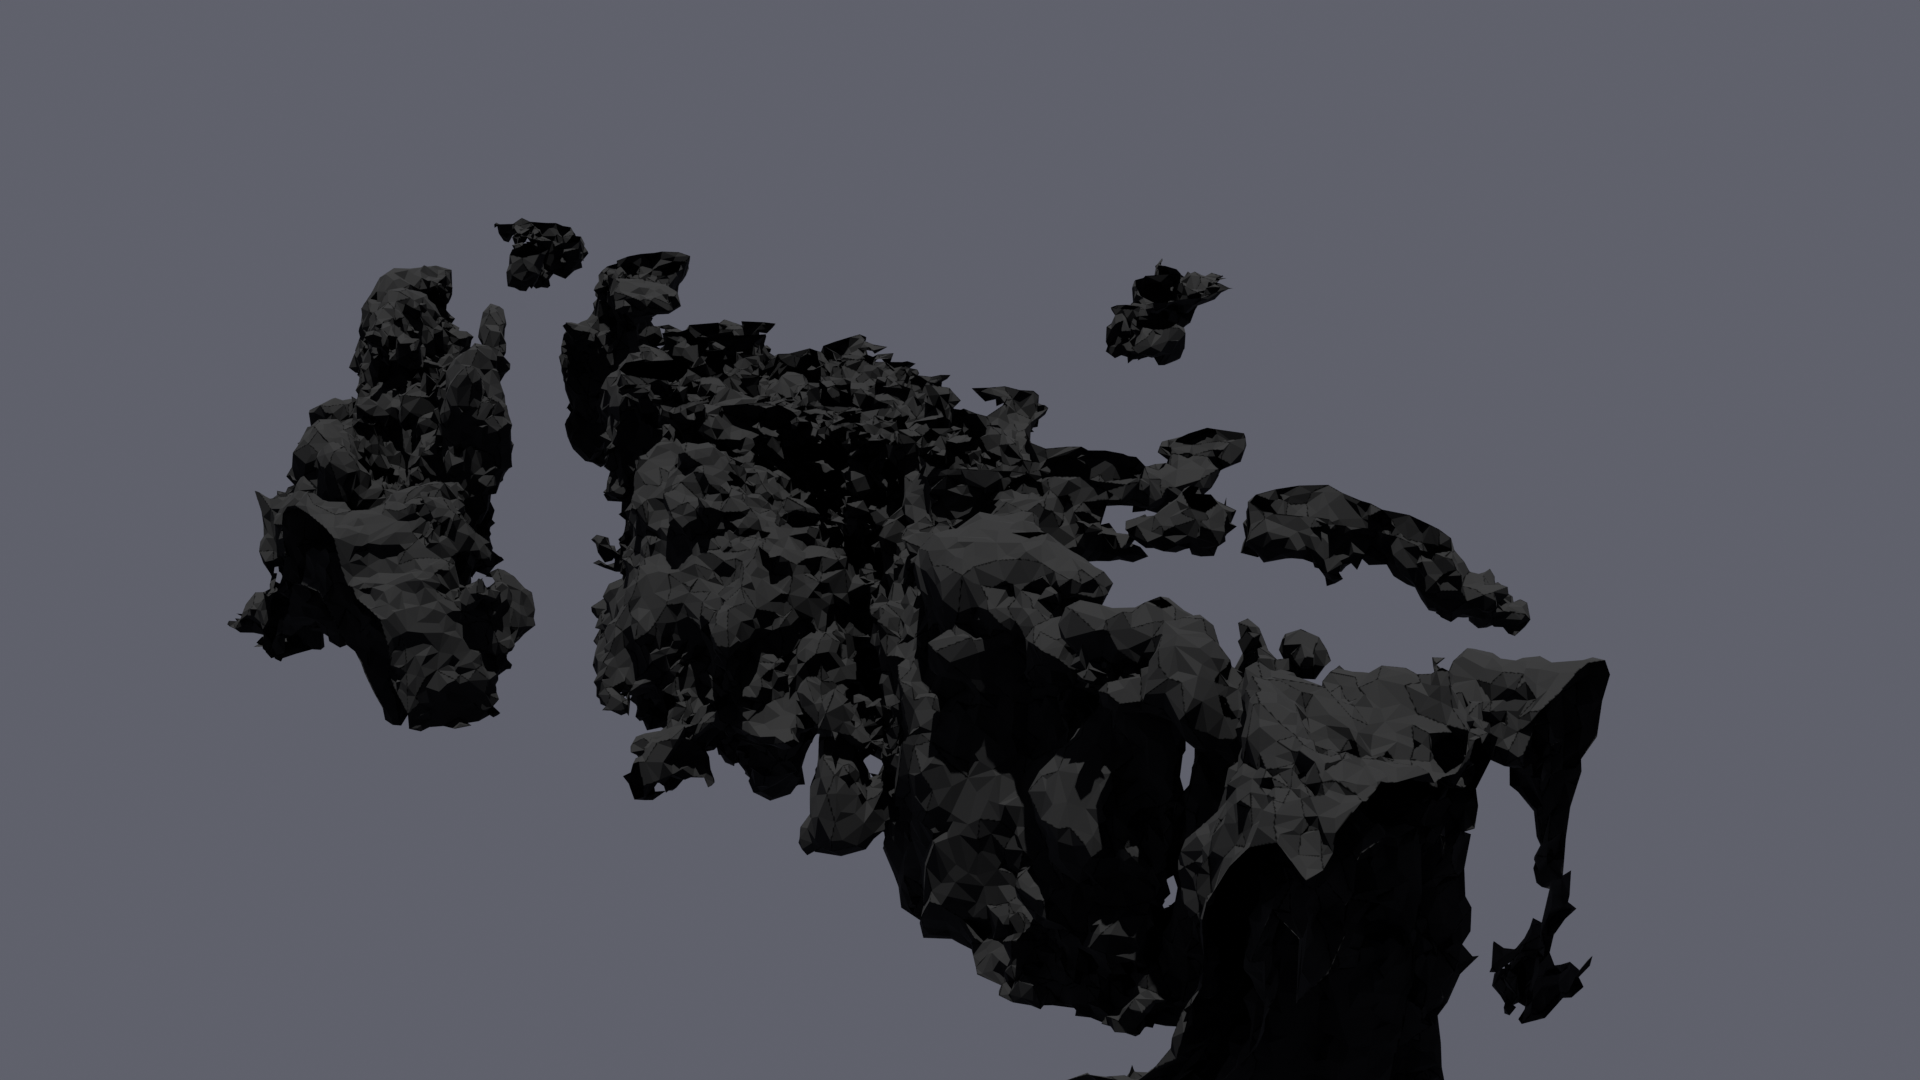
\includegraphics[width=0.85\textwidth]{v2/gsplat_mesh.png}
  \caption{Co-registered Gaussian splat (left) and extracted polygonal mesh (right)
    of a gallery interior captured with \texttt{gaussian-toolkit}.  The splat
    preserves specular highlights and fine texture detail; the mesh provides
    watertight geometry suitable for physics simulation, UV unwrapping, and
    engine import. Both representations are stored as \acrshort{usd} variants of
    the same scene prim and can be toggled without reloading scene metadata.}
  \label{fig:found-splat-mesh}
\end{figure}

% ────────────────────────────────────────────────────────────
\section{Surfaces from Splats}\label{sec:splats-to-surfaces}
% ────────────────────────────────────────────────────────────

A trained \acrshort{3dgs} scene is a point process of oriented ellipsoids, not a
surface. Primitives may overlap, interpenetrate, or float in empty space. Standard
mesh operations---UV unwrapping, Boolean difference, physics collision, real-time
\acrlong{pbr} shading---require a manifold surface representation. The extraction
of such a surface from a Gaussian splat field is an active research problem, and
the \texttt{gaussian-toolkit} exposes four distinct extraction backends to allow
trade-offs between geometric fidelity, computational cost, and output topology to
be made per-project.

\paragraph{The fundamental challenge.}
A Gaussian primitive contributes density continuously through space. Unlike a
neural \acrshort{tsdf} or an occupancy network, there is no obvious iso-surface.
Na\"{i}ve density thresholding produces ragged, topologically inconsistent meshes.
Extracting geometry that faithfully captures both large smooth walls and sub-centimetre
decorative relief from the same primitive set requires principled coupling between
the volumetric representation and the surface prior.

\paragraph{Surface-aligned methods.}
\textcite{Guedon2024Sugar} introduce SuGaR, which adds a regularisation term that
encourages each Gaussian to align its flattest axis with the nearest mesh surface
during training. A refined mesh is extracted by applying the Poisson surface
reconstruction algorithm to the aligned normals. SuGaR produces clean, manifold
meshes but requires a modified training loop; it is not applicable post-hoc to a
pre-trained splat.

\textcite{Guedon2025MILo} subsequently developed \acrlong{milo} (\acrshort{milo}),
which maintains a deformable mesh in the loop during splatting optimisation. The
mesh and the Gaussians are jointly optimised: the mesh constrains the positional
prior of nearby primitives while the photometric loss drives both simultaneously.
\acrshort{milo} achieves the highest surface quality in the benchmark comparison
presented in Chapter~\ref{ch:meshing} but doubles optimisation time relative to
standard training.

\paragraph{Post-hoc confidence-based extraction.}
\textcite{Radl2025CoMe} present \acrlong{come} (\acrshort{come}), which extracts
a mesh from a \emph{trained} splat without retraining by computing a per-primitive
confidence score derived from the accumulated photometric residual. High-confidence
primitives contribute surface normals to a spatially adaptive iso-surface;
low-confidence primitives are suppressed. \acrshort{come} is well-suited to the
\texttt{gaussian-toolkit} workflow because it operates as a post-processing step,
decoupling mesh quality from the choice of training configuration.

\paragraph{Gaussian wrapping.}
\textcite{Waczynska2024GaussianWrapping} approach the problem from the inverse
direction: rather than deriving a surface from density, they initialise a proxy
mesh and bind Gaussians to its faces, constraining primitive positions and
orientations to remain coherent with the mesh throughout optimisation. The
resulting \acrlong{gw} (\acrshort{gw}) representation is geometrically exact by
construction but requires a reasonable initial mesh---practically sourced from a
classical \acrshort{tsdf} reconstruction or an \acrshort{mvs} output.

\paragraph{Classical TSDF and marching cubes.}
The \acrlong{tsdf} \parencite{Curless1996} integrates per-view depth maps into a
volumetric signed-distance field on a voxel grid. The iso-surface at zero crossing
is extracted via the marching cubes algorithm \parencite{Lorensen1987}, producing
a triangle mesh whose resolution is determined by voxel spacing. In the
\texttt{gaussian-toolkit}, the \acrshort{tsdf} backend consumes depth maps rendered
from the trained splat rather than from a physical depth sensor, giving it access
to the fully optimised scene representation. Classical \acrshort{tsdf}+marching
cubes remains a competitively efficient baseline, especially for room-scale scenes
where the Gaussian normal field is sufficiently dense to produce artefact-free
depth renders.

A systematic empirical comparison of all four backends across geometry, run-time,
and perceptual quality metrics is deferred to Chapter~\ref{ch:meshing}.

% ────────────────────────────────────────────────────────────
\section{Promptable Segmentation}\label{sec:sam}
% ────────────────────────────────────────────────────────────

Scene decomposition into individually addressable objects is a prerequisite for
constructing a meaningful scene graph: a monolithic scene primitive cannot carry
per-object metadata, cannot be independently replaced with a generatively completed
mesh, and cannot be selected by a curator examining the scene in a browser viewer.

\paragraph{Segment Anything Model.}
\textcite{Kirillov2023} introduced \acrlong{sam} (\acrshort{sam}), a promptable
image segmentation foundation model trained on a dataset of over one billion masks.
Given a prompt in the form of a point, bounding box, or free-form mask, \acrshort{sam}
returns a segmentation of the corresponding object at interactive speed. The
promptable interface maps naturally onto the \texttt{gaussian-toolkit}'s interactive
web \acrshort{usd} viewer, where a curator can click an exhibit to trigger object
isolation.

\paragraph{SAM 2 for video-consistent decomposition.}
Image-level segmentation applied to individual video frames produces inconsistent
masks: the same object receives different segmentation boundaries in adjacent frames
due to motion blur, partial occlusion, and lighting change. \textcite{Ravi2024SAM2}
extend \acrshort{sam} to video with a streaming memory architecture that propagates
object-level mask tokens across frames. Given a prompt in a single frame,
\acrshort{sam}~2 tracks the corresponding object mask through the entire video
sequence, producing temporally consistent per-frame masks at up to 44 frames per
second on a single \acrshort{gpu}.

\paragraph{Lifting 2D masks to 3D consistency.}
The \texttt{gaussian-toolkit}'s segmentation module (\texttt{segment\_scene})
projects the per-frame \acrshort{sam}~2 masks back onto the trained Gaussian
primitive set via the calibrated cameras. Each primitive is assigned to the object
whose mask covers its projected centroid in the majority of frames in which it
is visible. This voting-based assignment is robust to single-frame mask failures
and produces 3D-consistent object labels without requiring any 3D supervision.
The labelled primitive subsets form the basis of the scene-graph decomposition
described in Chapter~\ref{ch:pipeline}, with each object's Gaussians isolated,
independently meshed, and associated with a distinct \acrshort{usd} prim.

% ────────────────────────────────────────────────────────────
\section{Generative 3D Reconstruction}\label{sec:generative}
% ────────────────────────────────────────────────────────────

A hand-held camera walkthrough systematically fails to observe the posterior
surface of any forward-facing exhibit. A showcase item presented against a wall
will have its back face entirely occluded throughout the capture; a sculpture on
a plinth may have its base inaccessible. Photogrammetric methods cannot reconstruct
surfaces they have never observed. The resulting holes in the mesh are either
filled by aggressive interpolation, which introduces geometrically incorrect
surface, or left open, which disqualifies the mesh from physical simulation and
game-engine import. For cultural heritage purposes, a complete object mesh---even
one whose occluded regions are generatively inferred---is of substantially greater
archival and display value than a fragment.

\paragraph{Multi-view diffusion.}
Multi-view diffusion models learn the joint distribution of object appearance
across a canonical set of viewpoints, conditioned on one or more observed views.
They encode strong shape priors from training on large 3D asset datasets and can
hallucinate plausible geometry for unobserved surfaces while remaining consistent
with the photographic evidence on the visible faces.

\textcite{Zhao2025Hunyuan} present Hunyuan3D~2.0, a two-stage system comprising
a multi-view diffusion model that synthesises consistent views at 24 canonical
camera positions and a reconstruction model that converts those views into a
textured mesh via differentiable rasterisation. Hunyuan3D~2.0 achieves state-of-the-art
quality on object-level reconstruction from a single image and scales to
high-resolution textures (up to $2048^2$ per chart).

\paragraph{ComfyUI orchestration.}
\texttt{gaussian-toolkit} executes Hunyuan3D~2.0 through \textcite{ComfyUI2024},
a modular, node-graph execution engine for diffusion pipelines. The \texttt{generate\_object\_mesh}
module constructs a \texttt{ComfyUI} workflow graph programmatically, submitting
each isolated object's best-observed view as a conditioning image and retrieving
the resulting textured mesh via the \texttt{ComfyUI} HTTP API. Using
\texttt{ComfyUI} as the execution layer decouples the \texttt{gaussian-toolkit}
from any specific model version: as Hunyuan3D or successor models are updated,
only the workflow JSON changes.

\paragraph{Background inpainting.}
Isolating an object for generative reconstruction exposes the background behind
it. Where the object partially occludes a wall or floor, the Gaussian splat
background shows a hole at those pixels. \texttt{gaussian-toolkit} employs
FLUX.1 \parencite{FLUX2024}---a rectified flow transformer trained for
high-fidelity text-conditioned image synthesis---as an inpainting model to fill
disoccluded background regions before they are incorporated into the scene's
background mesh. FLUX.1 is conditioned on the surrounding context pixels and a
brief natural-language description of the venue, generating texture-consistent
infill that avoids the conspicuous seams produced by classical patch-based methods.

\paragraph{Why generative completion is architecturally necessary.}
The decision to adopt generative completion rather than accept incomplete meshes
follows directly from the project's archival brief. A \acrshort{usd} scene intended
for long-term deposit must contain complete, watertight geometry for each registered
object. In the absence of completion, the pipeline would require a secondary capture
pass for every non-trivial exhibit---negating the single-capture design goal.
Generative completion introduces epistemic uncertainty on unseen faces, which is
acknowledged in the per-object metadata schema via a \texttt{completionConfidence}
field; downstream consumers can filter on this field if measured geometry is
preferred.

% ────────────────────────────────────────────────────────────
\section{Scene Description}\label{sec:usd}
% ────────────────────────────────────────────────────────────

The final output of \texttt{gaussian-toolkit} is not a single mesh or splat file
but a structured, hierarchical \emph{scene}---an environment mesh, a collection
of individually completed object meshes with metadata, and the original Gaussian
splat, all co-registered and jointly deliverable.

\paragraph{Universal Scene Description.}
\acrlong{usd} (\acrshort{usd}) \parencite{Pixar2019} is an open interchange
framework developed by Pixar Animation Studios and subsequently adopted across the
visual effects, games, and digital twin industries. Its core data model is a
hierarchy of typed \emph{prims} (primitives) that can carry geometry, material
bindings, camera definitions, light sources, and arbitrary user-defined metadata
attributes. Crucially, \acrshort{usd} supports \emph{composition arcs}---mechanisms
for layering, referencing, and instancing that allow large scenes to be assembled
from independently maintained asset files. For the \texttt{gaussian-toolkit}, the
relevant composition features are:

\begin{itemize}
  \item \textbf{Variant sets}: a named collection of alternative representations
    for a prim. Each scene object carries a \texttt{representation} variant set
    with two variants---\texttt{splat} (a reference to the Gaussian primitive
    subset) and \texttt{mesh} (a reference to the extracted or generatively
    completed polygonal mesh)---enabling renderer-appropriate view switching
    without duplicating scene topology.

  \item \textbf{Layer stacking}: the environment mesh, per-object assets, and
    splat data are authored in separate \texttt{.usda} or \texttt{.usdz} files
    and composed at the root stage level, so any layer can be updated in isolation
    without invalidating the others.

  \item \textbf{Custom schemas}: the \texttt{gaussian-toolkit} registers a
    lightweight \texttt{CulturalHeritageAPI} applied schema carrying fields for
    accession number, capture date, completionConfidence, and licensing, making
    the metadata intrinsically part of the geometry asset rather than a sidecar file.
\end{itemize}

\paragraph{Browser delivery.}
The \acrshort{usd} scene is the authoritative master format; browser delivery uses
derived representations. The Gaussian splat subset is exported as a \texttt{.ksplat}
file (the compressed container supported by \texttt{ksplat}, \acrshort{ksplat})
and streamed to a \acrlong{webgl} (\acrshort{webgl}) viewer based on the
open-source renderer of \textcite{Antimatter15Splat}. The emerging \acrlong{webgpu}
(\acrshort{webgpu}) standard \parencite{Khronos2024WebGPU}, which exposes
compute shaders in the browser, enables a more efficient tiled rasterisation path
that the \texttt{gaussian-toolkit} viewer activates automatically when the browser
reports \acrshort{webgpu} availability, falling back to \acrshort{webgl} otherwise.
Polygon meshes are served as compressed \texttt{glTF~2.0} with Draco-encoded
geometry, enabling the same delivery infrastructure used for standard web 3D
content.

\paragraph{Summary.}
The six technology strata described in this chapter---\acrshort{sfm}/\acrshort{mvs}
pose recovery, \acrshort{3dgs} volumetric representation, post-hoc mesh extraction,
\acrshort{sam}~2 video segmentation, multi-view generative completion, and
\acrshort{usd} scene composition---form an engineering stack in which each layer
consumes the output of its predecessor. No layer has a fundamental dependency on
the specific implementation choice of any other: the meshing backends are
interchangeable, the generative model is invoked through an abstracted
\texttt{ComfyUI} graph, and the \acrshort{usd} representation is independent of
the delivery target. This composability is the architectural principle that allows
\texttt{gaussian-toolkit} to accommodate methodological advances in any single
layer without redesigning the pipeline as a whole.

% v2_ch3_pipeline.tex — Chapter 3: Pipeline Architecture
% Video-to-Gaussian: An Agentic Pipeline for Volumetric Cultural Heritage Preservation
% Dr John O'Hare, DreamLab AI Consulting Ltd — June 2026

\chapter{Pipeline Architecture}\label{ch:pipeline}

The \texttt{gaussian-toolkit} is not a shell script that glues together pre-existing tools;
it is a purposefully architected system in which an \acrshort{llm} orchestrator reasons
about state, selects tool calls, handles retries, and passes structured artefacts between
bounded contexts. This chapter documents the design principles that shaped that architecture,
the eight processing stages executed for every acquisition, the three-container compute
fabric that hosts them, the hardware platform, and the control surfaces through which
operators interact with the running system.

% ─────────────────────────────────────────────────────────────────────────────
\section{Design Principles}\label{sec:design-principles}
% ─────────────────────────────────────────────────────────────────────────────

\subsection{Domain-Driven Design and Bounded Contexts}

The architecture follows \acrfull{ddd}, partitioning responsibility into seven
bounded contexts whose interfaces are explicit and whose internal implementations
may evolve independently:

\begin{description}[leftmargin=2.4cm, labelwidth=2.2cm]
  \item[Capture]        Ingestion of raw video, temporal decimation, and candidate-frame storage.
  \item[Reconstruction] Keyframe selection, \acrshort{colmap} \acrshort{sfm}, and
                        \acrshort{3dgs} model training — the photogrammetric core.
  \item[Segmentation]   Object-level decomposition of the Gaussian field via \acrshort{sam}~2
                        and cluster validation.
  \item[Generative-Reconstruction] Per-object orbit rendering, Hunyuan3D~2.0 mesh generation,
                        and \acrshort{pbr} texturing via FLUX inpainting.
  \item[Meshing]        Whole-scene surface reconstruction using one of four configurable backends.
  \item[Assembly]       Construction of the hierarchical \acrshort{usd} scene graph and
                        emplacement of reconstructed objects at \acrshort{colmap}-derived centroids.
  \item[Delivery]       Export to \texttt{.ksplat} for browser streaming, plus optional
                        \acrshort{webgl}/\acrshort{webgpu} viewer deployment.
\end{description}

Bounded contexts communicate through well-typed data contracts: frame manifests (JSON),
camera parameter files (\texttt{transforms.json}), Gaussian \texttt{.ply} archives, mask
HDF5 files, and \acrshort{usd} stage references. No context reads another's internal state directly.

\subsection{Architecture Decision Records}

All non-trivial design choices are captured as \acrfull{adr}s, versioned alongside the
source code. Two records are directly relevant to the compute fabric described in
Section~\ref{sec:containers}:

\begin{itemize}
  \item \textbf{ADR-001} (\emph{Container isolation per CUDA ABI}) — mandates one Docker
        image per incompatible CUDA/\-PyTorch combination, communicating via a shared NVMe
        volume and a lightweight REST job-handoff protocol, rather than attempting
        multi-environment conda workarounds inside a single container.
  \item \textbf{ADR-002} (\emph{GPU affinity assignment}) — binds the primary reconstruction
        workload exclusively to GPU~0 and delegates all sidecar meshing to GPU~1, preventing
        VRAM contention during the densification-intensive \acrshort{3dgs} training phase.
\end{itemize}

\subsection{Agentic Orchestration}

Conventional multi-stage photogrammetry pipelines are driven by shell scripts that invoke
tools in a fixed order and abort on the first non-zero exit code. \texttt{gaussian-toolkit}
replaces this with an \acrshort{llm} orchestrator connected to \acrshort{mcp} server
running on port 45677, which exposes over 70 tools covering every stage. The orchestrator
reasons about intermediate quality metrics — checking reprojection error before proceeding
to training, validating cluster coverage before initiating generative reconstruction — and
can reroute execution, adjust hyperparameters, or surface diagnostic messages to the
operator without human intervention. This makes the system resilient to the variability
inherent in real gallery footage: inconsistent lighting, partial occlusion, and
camera shake that would cause a brittle script to fail silently.

% ─────────────────────────────────────────────────────────────────────────────
\section{The Eight-Stage Pipeline}\label{sec:pipeline-stages}
% ─────────────────────────────────────────────────────────────────────────────

Figure~\ref{fig:pipeline-flow} illustrates the eight stages executed for a single
acquisition. Stages 1–4 constitute the photogrammetric core and are described in
detail below. Stages 5–8 are documented in the dedicated chapters that follow
(Chapter~\ref{ch:scenegraph} covers segmentation and \acrshort{usd} assembly;
Chapter~\ref{ch:meshing} covers environment meshing); a brief description of each
is included here for completeness.

\begin{figure}[htbp]
\centering
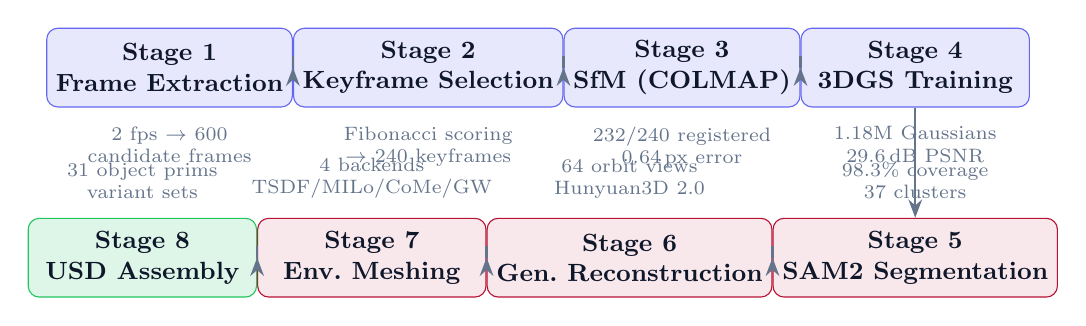
\begin{tikzpicture}[
  node distance = 0.55cm and 0.0cm,
  stage/.style  = {draw, rounded corners=4pt, minimum width=2.9cm,
                   minimum height=1.0cm, align=center, font=\small\bfseries,
                   fill=LightGrey, draw=MidGrey, text=DarkBg},
  arrow/.style  = {-Stealth, thick, color=MidGrey},
  label/.style  = {font=\scriptsize, text=MidGrey, align=center}
]
  % Row 1: stages 1-4
  \node[stage, fill=DreamLabAccent!15, draw=DreamLabAccent] (s1) {Stage 1\\Frame Extraction};
  \node[stage, fill=DreamLabAccent!15, draw=DreamLabAccent, right=of s1] (s2) {Stage 2\\Keyframe Selection};
  \node[stage, fill=DreamLabAccent!15, draw=DreamLabAccent, right=of s2] (s3) {Stage 3\\SfM (COLMAP)};
  \node[stage, fill=DreamLabAccent!15, draw=DreamLabAccent, right=of s3] (s4) {Stage 4\\3DGS Training};

  % Row 2: stages 5-8 (below, right-to-left for visual return)
  \node[stage, fill=UoSRed!10, draw=UoSRed, below=1.4cm of s4] (s5) {Stage 5\\SAM2 Segmentation};
  \node[stage, fill=UoSRed!10, draw=UoSRed, left=of s5] (s6) {Stage 6\\Gen.\ Reconstruction};
  \node[stage, fill=UoSRed!10, draw=UoSRed, left=of s6] (s7) {Stage 7\\Env.\ Meshing};
  \node[stage, fill=SuccessGreen!15, draw=SuccessGreen, left=of s7] (s8) {Stage 8\\USD Assembly};

  % Row 1 arrows
  \draw[arrow] (s1) -- (s2);
  \draw[arrow] (s2) -- (s3);
  \draw[arrow] (s3) -- (s4);

  % Turn arrow s4 -> s5
  \draw[arrow] (s4) -- (s5);

  % Row 2 arrows (right to left)
  \draw[arrow] (s5) -- (s6);
  \draw[arrow] (s6) -- (s7);
  \draw[arrow] (s7) -- (s8);

  % Annotations below row 1
  \node[label, below=0.12cm of s1] {2 fps $\to$ 600\\candidate frames};
  \node[label, below=0.12cm of s2] {Fibonacci scoring\\$\to$ 240 keyframes};
  \node[label, below=0.12cm of s3] {232/240 registered\\0.64\,px error};
  \node[label, below=0.12cm of s4] {1.18M Gaussians\\29.6\,dB PSNR};

  % Annotations above row 2
  \node[label, above=0.12cm of s5] {98.3\% coverage\\37 clusters};
  \node[label, above=0.12cm of s6] {64 orbit views\\Hunyuan3D 2.0};
  \node[label, above=0.12cm of s7] {4 backends\\TSDF/MILo/CoMe/GW};
  \node[label, above=0.12cm of s8] {31 object prims\\variant sets};

\end{tikzpicture}
\caption{The eight-stage \texttt{gaussian-toolkit} pipeline. Stages 1–4 (blue) form the
  photogrammetric core; stages 5–7 (red) perform semantic decomposition, generative
  reconstruction, and surface meshing; stage 8 (green) assembles the hierarchical
  \acrshort{usd} scene graph.}
\label{fig:pipeline-flow}
\end{figure}

\subsection{Stage 1 — Frame Extraction}

Raw 4K gallery footage is ingested via \texttt{ffmpeg} with a temporal decimation rate
of 2 frames per second. For a typical 5-minute acquisition walk this yields approximately
600 candidate frames, stored as lossless PNG at full sensor resolution. The module
\texttt{frame\_extractor.py} writes a JSON manifest alongside each batch recording
source timecode, frame index, and a SHA-256 hash of the pixel buffer. The manifest
serves as a checkpoint: if the pipeline is interrupted and resumed, frames already
extracted are skipped without re-decoding.

\subsection{Stage 2 — Keyframe Selection}

Six hundred candidate frames are far too many for efficient \acrshort{sfm} registration
and introduce redundant viewpoints that inflate the subsequent Gaussian count without
improving quality. The module \texttt{fibonacci\_sampler.py} implements a Fibonacci-sphere
viewpoint scoring heuristic in which each candidate is assigned a composite score

\[
  s_i = 0.6\,\sigma_i + 0.4\,\kappa_i
\]

\noindent where $\sigma_i$ is a normalised sharpness score (Laplacian variance, max-pooled
over $32\times32$ tiles) and $\kappa_i$ is a coverage score measuring angular distance from
the nearest already-selected keyframe on the Fibonacci sphere approximation of the view
hemisphere. The top 240 frames by composite score are retained, reducing the set by 60\%
while preserving broad angular coverage. In practice this selection consistently improves
\acrshort{sfm} registration rate compared to uniform temporal subsampling, because blurry
or redundant frames that degrade feature matching are preferentially excluded.

\subsection{Stage 3 — Structure-from-Motion}

The 240 selected keyframes are passed to \acrshort{colmap}~\citep{Schoenberger2016sfm,
Schoenberger2016mvs} running in sequential-mapper mode with SIFT~\citep{Lowe2004} features.
For the reference gallery acquisition, 232 of 240 frames registered successfully
(96.7\,\%), yielding a sparse point cloud of approximately 210,000 points with a
mean reprojection error of 0.64\,px — comfortably within the $<1$\,px threshold that
reliably produces well-conditioned Gaussian initialisation. The eight unregistered frames
were all affected by severe motion blur during camera panning at the gallery perimeter;
the Fibonacci scoring step eliminated most such frames, but eight passed the sharpness
threshold because blur was localised to a small tile.

Camera intrinsics and extrinsics are exported to \texttt{transforms.json} in the
NeRFStudio/\allowbreak{}LichtFeld-Studio format. A secondary \texttt{cameras.bin} export
is retained for downstream TSDF meshing, which requires COLMAP-native binary format.

\subsection{Stage 4 — 3DGS Training}

Gaussian splatting training is performed by \texttt{LichtFeld Studio}~\citep{LichtFeldStudio2026},
the Inria-licensed viewer and training harness that forms the upstream of the
\texttt{gaussian-toolkit} fork. Training runs for 30,000 iterations with the
\acrfull{mrnf} densification strategy, which applies a surface-normal consistency
filter during the adaptive density control loop to suppress needle-like floater Gaussians
in low-texture regions such as painted wall surfaces.

On the reference hardware (GPU~0, RTX~6000 Ada, 48\,GB VRAM) training completes in
24 minutes, converging to 1.18 million Gaussians. Hold-out evaluation on 12 reserved
frames yields:

\begin{itemize}
  \item \acrshort{psnr}: $29.6$\,dB
  \item \acrshort{ssim}: $0.921$
  \item \acrshort{lpips}: $0.108$
\end{itemize}

The trained splat renders at 160 frames per second at 1080p on the same GPU, meeting the
real-time interactive threshold with comfortable headroom for simultaneous web streaming.
The model is exported both as a raw \texttt{.ply} (for downstream segmentation and meshing)
and as a compressed \texttt{.ksplat} (for browser delivery via \acrshort{webgl}).

\subsection{Stages 5–8 — Overview}

\textbf{Stage~5 (Segmentation)} applies \acrshort{sam}~2~\citep{Ravi2024SAM2} across all
240 registered views to produce per-Gaussian cluster assignments. The full segmentation
workflow, cluster validation criteria, and the mask projection module
\texttt{mask\_projector.py} are described in Chapter~\ref{ch:scenegraph}.

\textbf{Stage~6 (Generative reconstruction)} renders 64 orbit views per retained cluster
and passes them to Hunyuan3D~2.0~\citep{Zhao2025Hunyuan} via ComfyUI (port 8188) to
generate a watertight \acrshort{pbr}-textured mesh for each object. FLUX~\citep{FLUX2024}
inpainting resolves seam artefacts. This stage is also documented in
Chapter~\ref{ch:scenegraph}.

\textbf{Stage~7 (Environment meshing)} reconstructs the room envelope and large static
surfaces using one of four selectable backends (\acrshort{tsdf}~\citep{Curless1996},
\acrshort{milo}~\citep{Guedon2025MILo}, \acrshort{come}~\citep{Radl2025CoMe}, or
Gaussian Wrapping). Backend selection and quality trade-offs are analysed in
Chapter~\ref{ch:meshing}.

\textbf{Stage~8 (USD assembly)} constructs a hierarchical \acrshort{usd} scene
graph~\citep{Pixar2019} with 31 object prims emplaced at \acrshort{colmap}-derived
centroids. Each prim carries a variant set offering both a Gaussian splat representation
and a mesh representation, enabling downstream consumers to select the appropriate fidelity
tier. Assembly is also covered in Chapter~\ref{ch:scenegraph}.

% ─────────────────────────────────────────────────────────────────────────────
\section{Three-Container Compute Fabric}\label{sec:containers}
% ─────────────────────────────────────────────────────────────────────────────

The three meshing backends — \acrshort{milo}, \acrshort{come}, and Gaussian Wrapping —
each require PyTorch extension modules compiled against specific CUDA toolkit versions
that are mutually incompatible: \acrshort{milo} requires CUDA~11.8 and PyTorch~2.0,
\acrshort{come} requires CUDA~12.1 and PyTorch~2.3, and the primary
\texttt{gaussian-toolkit} container targets CUDA~12.8 and PyTorch~2.7 for
access to the latest Hopper/Ada optimisations in the Gaussian rasteriser.
Installing all three in a single environment via conda is not feasible without
breaking at least one set of compiled extensions.

ADR-001 resolves this by mandating one Docker image per CUDA ABI. The three containers
communicate through two mechanisms: a shared NVMe Docker volume
(\texttt{gaussian-shared-vol}) that carries large binary artefacts (Gaussian \texttt{.ply}
files, depth maps, mesh outputs), and a lightweight REST job-handoff protocol in which
\texttt{gaussian-toolkit} POSTs a job descriptor to each sidecar container's local
Flask server and polls for completion. This keeps container interfaces narrow and avoids
the complexity of a full message broker for what is, in practice, a sequential handoff
with at most two concurrent sidecar jobs.

Table~\ref{tab:containers} summarises the three containers and their responsibilities.

\begin{table}[htbp]
\centering
\caption{Three-container compute fabric: CUDA environments and responsibilities.}
\label{tab:containers}
\begin{tabular}{@{}L{3.2cm} C{1.5cm} C{1.5cm} C{1.4cm} L{6.0cm}@{}}
\toprule
\textbf{Container} & \textbf{CUDA} & \textbf{Python} & \textbf{GPU} & \textbf{Responsibilities} \\
\midrule
\texttt{gaussian-toolkit} & 12.8 & 3.12 & GPU~0 &
  Orchestration, frame extraction, \acrshort{colmap} \acrshort{sfm},
  \acrshort{3dgs} training (\acrshort{mrnf} densification),
  \acrshort{tsdf} meshing, \acrshort{sam}~2 segmentation,
  mask projection, \acrshort{usd} assembly,
  \texttt{.ksplat} export, web UI and ttyd terminal. \\[4pt]
\texttt{milo} & 11.8 & 3.10 & GPU~1 &
  \acrfull{milo} mesh-in-the-loop optimisation;
  Gaussian Wrapping backend. \\[4pt]
\texttt{come} & 12.1 & 3.10 & GPU~1 &
  \acrfull{come} confidence-based surface extraction. \\
\bottomrule
\end{tabular}
\end{table}

\begin{figure}[htbp]
\centering
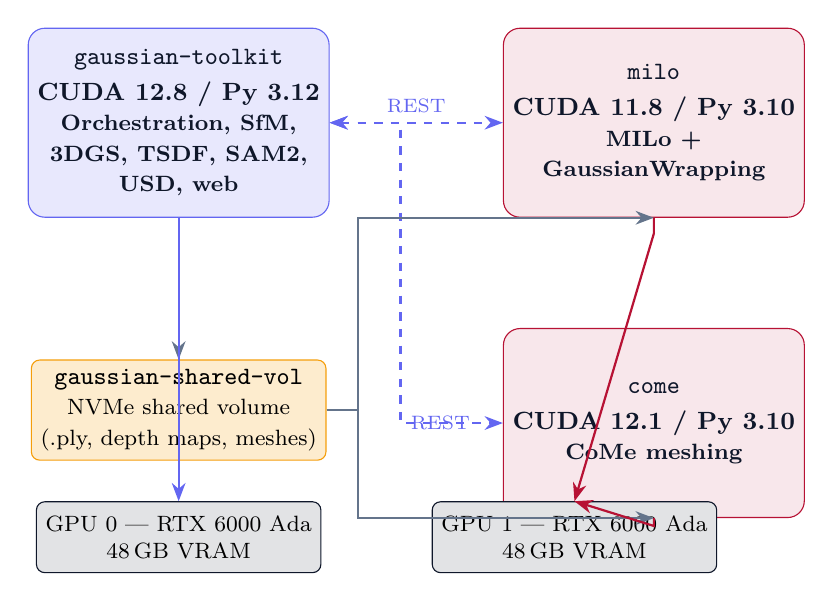
\begin{tikzpicture}[
  node distance  = 1.0cm and 1.2cm,
  container/.style = {draw, rounded corners=6pt, minimum width=3.6cm,
                      minimum height=2.4cm, align=center, font=\small\bfseries,
                      text=DarkBg},
  gpu/.style       = {draw, rounded corners=3pt, minimum width=3.0cm,
                      minimum height=0.9cm, align=center, font=\footnotesize,
                      fill=DarkBg!12, draw=DarkBg},
  vol/.style       = {draw, rounded corners=3pt, minimum width=3.2cm,
                      minimum height=1.0cm, align=center, font=\small,
                      fill=WarningAmber!20, draw=WarningAmber},
  arrow/.style     = {-Stealth, thick, color=MidGrey},
  restarrow/.style = {Stealth-Stealth, thick, color=DreamLabAccent, dashed}
]

  % Primary container
  \node[container, fill=DreamLabAccent!15, draw=DreamLabAccent] (gt) {
    \texttt{gaussian-toolkit}\\[2pt]
    CUDA 12.8 / Py 3.12\\
    \footnotesize Orchestration, SfM,\\
    \footnotesize 3DGS, TSDF, SAM2,\\
    \footnotesize USD, web
  };

  % Sidecar containers
  \node[container, fill=UoSRed!10, draw=UoSRed, right=2.2cm of gt] (milo) {
    \texttt{milo}\\[2pt]
    CUDA 11.8 / Py 3.10\\
    \footnotesize MILo +\\
    \footnotesize GaussianWrapping
  };

  \node[container, fill=UoSRed!10, draw=UoSRed, below=1.4cm of milo] (come) {
    \texttt{come}\\[2pt]
    CUDA 12.1 / Py 3.10\\
    \footnotesize CoMe meshing
  };

  % Shared volume
  \node[vol, below=1.8cm of gt] (vol) {
    \texttt{gaussian-shared-vol}\\
    \footnotesize NVMe shared volume\\
    \footnotesize (.ply, depth maps, meshes)
  };

  % GPU nodes
  \node[gpu, below=3.6cm of gt] (gpu0) {GPU 0 — RTX 6000 Ada\\48\,GB VRAM};
  \node[gpu, right=1.4cm of gpu0] (gpu1) {GPU 1 — RTX 6000 Ada\\48\,GB VRAM};

  % Arrows: REST job handoff
  \draw[restarrow] (gt.east) -- node[above,font=\scriptsize,text=DreamLabAccent]{REST} (milo.west);
  \draw[restarrow] (gt.east) -- ++(0.9,0) |- node[right,font=\scriptsize,text=DreamLabAccent]{REST} (come.west);

  % Arrows: shared volume
  \draw[arrow] (gt.south) -- (vol.north);
  \draw[arrow] (vol.east) -- ++(0.4,0) |- (milo.south);
  \draw[arrow] (vol.east) -- ++(0.4,0) |- (come.south);

  % GPU assignments
  \draw[arrow, color=DreamLabAccent] (gt.south) -- ++(0,-0.15) -- (gpu0.north);
  \draw[arrow, color=UoSRed] (milo.south) -- ++(0,-0.2) -- (gpu1.north);
  \draw[arrow, color=UoSRed] (come.south) -- ++(0,-0.1) -- (gpu1.north);

\end{tikzpicture}
\caption{Three-container compute fabric. The primary \texttt{gaussian-toolkit} container
  (blue) orchestrates sidecar containers \texttt{milo} and \texttt{come} (red) via REST
  job descriptors and a shared NVMe volume. GPU affinity follows ADR-002: GPU~0 for
  reconstruction, GPU~1 for sidecar meshing.}
\label{fig:containers}
\end{figure}

% ─────────────────────────────────────────────────────────────────────────────
\section{Hardware Platform}\label{sec:hardware}
% ─────────────────────────────────────────────────────────────────────────────

All experiments reported in this document were conducted on a single workstation
configured as follows:

\begin{itemize}
  \item \textbf{GPUs}: dual NVIDIA RTX~6000 Ada Generation, 48\,GB GDDR6 ECC each
        (96\,GB total \acrshort{vram}). GPU~0 handles the complete reconstruction
        pipeline; GPU~1 is reserved exclusively for sidecar meshing workloads,
        preventing the memory pressure that would otherwise arise from running
        \acrshort{milo} or \acrshort{come} concurrently with a live \acrshort{3dgs}
        model in GPU~0 VRAM.
  \item \textbf{CPU}: AMD Threadripper PRO, 48 physical cores. The high core count
        benefits the \acrshort{colmap} feature-matching and bundle-adjustment phases,
        which parallelise efficiently across CPU threads before the GPU rasteriser
        dominates in later stages.
  \item \textbf{System RAM}: 251\,GB DDR5 ECC. Large system RAM allows the full
        candidate frame set (600 frames at 4K PNG, approximately 28\,GB) to reside
        in RAM throughout the pipeline, eliminating NVMe I/O latency during repeated
        reads by the SIFT extractor.
  \item \textbf{Storage}: NVMe SSD array hosting the shared Docker volume; sequential
        read bandwidth in excess of 12\,GB/s sustains the depth-map streaming rates
        required by \acrshort{tsdf} fusion without introducing pipeline stalls.
\end{itemize}

The 96\,GB combined \acrshort{vram} budget is not exhausted by the reference acquisition:
\acrshort{3dgs} training with 1.18\,M Gaussians peaks at approximately 18\,GB on GPU~0,
leaving substantial headroom for larger scenes or higher Gaussian counts in future
acquisitions. GPU~1 headroom (typically 6–12\,GB utilised by sidecar meshing) permits
the concurrent execution of multiple meshing backend comparisons without swapping.

% ─────────────────────────────────────────────────────────────────────────────
\section{Agentic Control Surface}\label{sec:control-surface}
% ─────────────────────────────────────────────────────────────────────────────

The operator's primary interface to the running pipeline is the \acrshort{mcp} server
embedded in \texttt{gaussian-toolkit}, which listens on port~45677 and exposes
over 70 typed tool calls. These tools span every bounded context: from
\texttt{ingest\_video} and \texttt{run\_colmap} at the front of the pipeline,
through \texttt{train\_3dgs}, \texttt{run\_sam2}, and \texttt{dispatch\_hunyuan},
to \texttt{assemble\_usd} and \texttt{export\_ksplat} at the delivery end.

The \acrshort{llm} orchestrator connects to this \acrshort{mcp} server and drives
the pipeline by issuing tool calls, inspecting return values (which include structured
quality metrics and error codes), and deciding whether to proceed, adjust a
hyperparameter, or surface an alert. This architecture cleanly separates the
\emph{reasoning layer} (the orchestrator, which can be swapped for any
\acrshort{mcp}-compatible client) from the \emph{execution layer} (the toolkit,
which exposes a stable tool API). Operators can also invoke tools directly from any
\acrshort{mcp} client, enabling ad-hoc inspection and intervention without modifying
the pipeline code.

Two secondary control surfaces are provided for human operators who prefer a graphical
or terminal interface. The web \acrshort{ui} (Figure~\ref{fig:webui}) presents a
dashboard summarising pipeline state, live training metrics (loss, PSNR, iteration
count), and GPU utilisation. The ttyd terminal (Figure~\ref{fig:ttyd}) exposes a full
shell inside the \texttt{gaussian-toolkit} container through a browser tab, enabling
direct inspection of intermediate artefacts, log files, and the \acrshort{colmap}
workspace without requiring SSH access.

\begin{figure}[htbp]
  \centering
  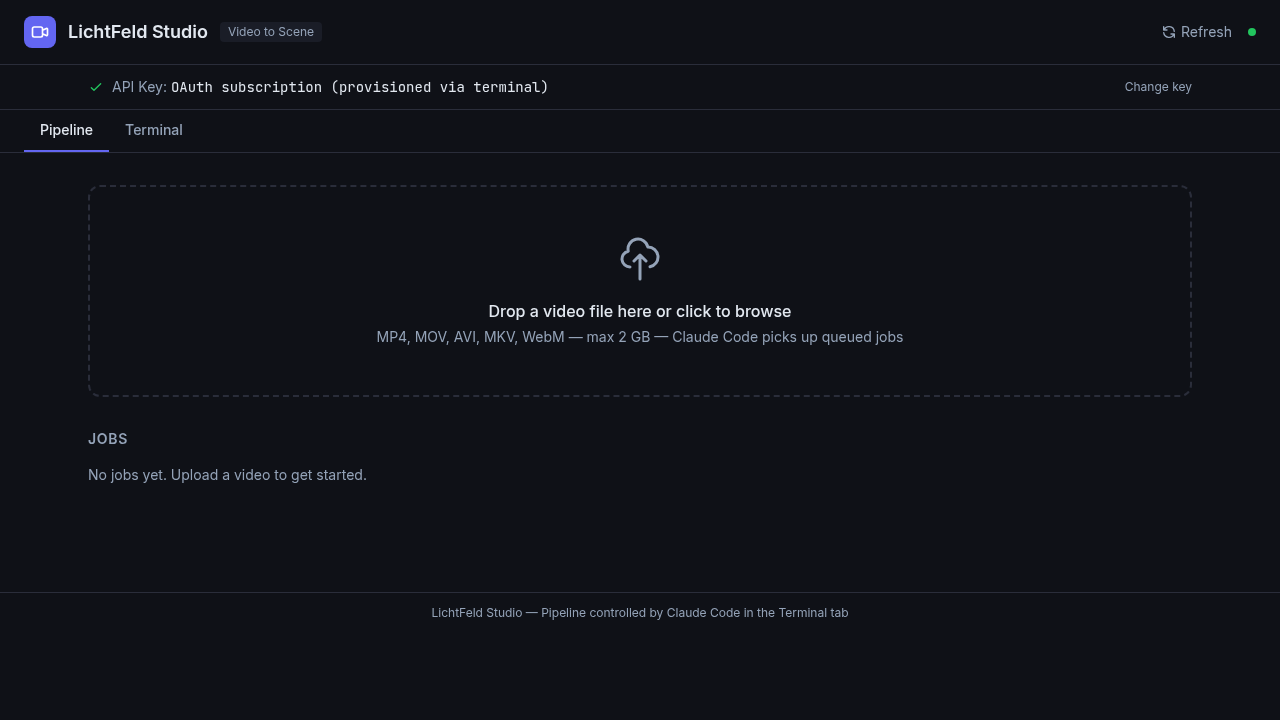
\includegraphics[width=0.8\textwidth]{v2/webui.png}
  \caption{The \texttt{gaussian-toolkit} web control interface, showing pipeline stage
    status, live \acrshort{3dgs} training metrics, and \acrshort{gpu} telemetry.}
  \label{fig:webui}
\end{figure}

\begin{figure}[htbp]
  \centering
  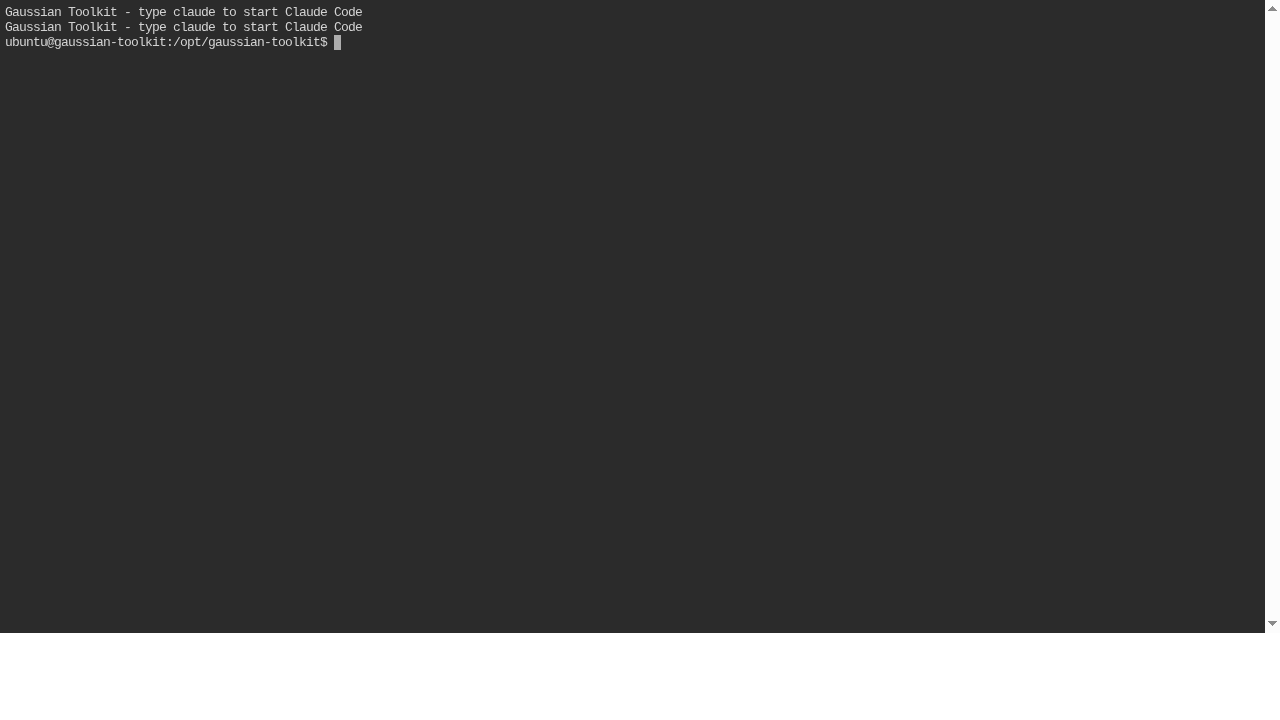
\includegraphics[width=0.8\textwidth]{v2/ttyd.png}
  \caption{The ttyd browser terminal embedded in the \texttt{gaussian-toolkit} web
    interface, providing in-browser shell access to the container for direct artefact
    inspection and ad-hoc tool invocation.}
  \label{fig:ttyd}
\end{figure}

\begin{keyfinding}
  The combination of \acrshort{mcp}-mediated agentic orchestration with direct web and
  terminal control surfaces allows \texttt{gaussian-toolkit} to be operated both
  fully autonomously (the orchestrator drives all 8 stages without human input) and
  interactively (an operator inspects intermediate artefacts and overrides decisions at
  any stage boundary). Neither mode requires modifying pipeline code.
\end{keyfinding}

% Chapter 4 — Integrating LichtFeld Studio v0.5.2
% Video-to-Gaussian: An Agentic Pipeline for Volumetric Cultural Heritage Preservation
% Dr John O'Hare, DreamLab AI Consulting Ltd
% v2.0 — June 2026

\chapter{Integrating LichtFeld Studio v0.5.2}
\label{ch:lichtfeld}

The v1.0 pilot proved that \acrshort{3dgs}~\parencite{Kerbl2023} was a viable medium for heritage preservation.
Its bespoke trainer, however, was a maintenance liability: every advance in densification strategy, rasteriser
performance, or export format required hand-porting rather than a simple upstream pull.
This chapter documents how the v2.0 system was re-platformed onto
LichtFeld~Studio~v0.5.2~\parencite{LichtFeldStudio2026} (git tag \texttt{d9e76009}, dated 2026-04-21)
and describes the specific capabilities that upgrade delivered to the heritage capture workflow.

% ─────────────────────────────────────────────────────────────────────────────
\section{Rationale for Re-Platforming}
\label{sec:lf-rationale}
% ─────────────────────────────────────────────────────────────────────────────

The v1.0 bespoke trainer grew organically from an early open-source \acrshort{3dgs} reference implementation.
Over approximately eighteen months it accumulated local patches for multi-resolution densification, a
custom CUDA rasteriser backport, and ad-hoc export routines for \texttt{.ply} and \texttt{.splat} containers.
Each of those additions was written against internal data structures that diverged progressively from the
community codebase, making it increasingly difficult to absorb improvements from the research stream
without substantial merge effort.

LichtFeld~Studio emerged as the community's de-facto maintained distribution of \acrshort{3dgs} tooling.
By v0.5.2 it combined a rigorously benchmarked CUDA rasteriser, a non-destructive editing suite, native
\acrshort{usd} I/O, an in-application quality-evaluation mode, and a programmatic \acrshort{mcp} control
surface — each component maintained by a community with a faster release cadence than a single-institution
project can sustain.

The re-platforming decision was therefore primarily an exercise in reducing bespoke code surface.
The \texttt{gaussian-toolkit} fork tracks 215 upstream commits to the v0.5.2 tag and adds only the
integration layer described in this chapter: scene-graph mapping, orchestrator bindings, and the
quality-gating logic that consumes evaluation metrics from the engine.
All reconstruction logic, the CUDA rasteriser, densification strategies (\acrshort{mcmc},
\acrshort{mrnf}), and mesh-extraction backend stubs reside in the upstream codebase.
This arrangement allows the toolkit to absorb research velocity from the LichtFeld community
while confining heritage-specific concerns to a thin, reviewable integration layer.

% ─────────────────────────────────────────────────────────────────────────────
\section{Scene-Graph Harmonisation}
\label{sec:lf-scenegraph}
% ─────────────────────────────────────────────────────────────────────────────

Upstream commit \texttt{34e2ba85} introduced what the LichtFeld project calls
\emph{scene-graph harmonisation}: a unified internal node hierarchy that supersedes the earlier
flat list of Gaussian primitive arrays.
Prior to that commit, the trainer maintained Gaussians as unstructured parameter tensors with no
persistent identity across training iterations; exporting a scene meant serialising the full tensor
state into a monolithic \texttt{.ply} file.
After harmonisation, every Gaussian is assigned to a named node in an acyclic hierarchy, and the
hierarchy itself is preserved across checkpoint saves and resumes.

The toolkit's integration layer maps this harmonised node hierarchy onto \acrshort{usd}
prims~\parencite{Pixar2019} at export time using a deterministic naming convention:
each internal node identifier becomes a USD \texttt{Xform} prim path, and the Gaussian
payload attached to that node becomes a nested \texttt{PointInstancer} or
\texttt{GaussianSplat} schema prim depending on downstream consumer preference.
The result is a clean, one-to-one correspondence between the trainer's internal scene structure
and the exported USD scene graph.

This correspondence is the key enabler of the hierarchical export described in
Chapter~\ref{ch:scenegraph}.
Because the mapping is defined by node names rather than tensor indices, it is stable across
re-training runs and amenable to manual curation: a conservator may rename or reparent nodes in the
USD file and re-import them into the trainer without corruption.
The scene graph therefore functions as the shared address space that binds the training engine,
the editing suite, and the downstream assembly pipeline into a single coherent workflow.

% ─────────────────────────────────────────────────────────────────────────────
\section{Native USD I/O}
\label{sec:lf-usd}
% ─────────────────────────────────────────────────────────────────────────────

LichtFeld~Studio~v0.5.2 introduced a first-class \acrshort{usd} layer built on the
OpenUSD C++ libraries~\parencite{Pixar2019}, exposing bidirectional scene
read and write from within the training process itself.
Earlier workflows required a post-training conversion step: the trainer emitted \texttt{.ply},
a separate tool converted to USD, and any editing performed in a USD-aware host had to be
re-imported through a lossy round-trip.

Under the native I/O model the trainer reads initial point-cloud priors directly from a USD layer,
preserves camera rig geometry as USD camera prims, and checkpoints the Gaussian field into a
\texttt{.usda}/\texttt{.usdz} stage at each evaluation interval.
The editing suite — responsible for splat culling, object segmentation, and manual correction —
opens the same USD stage, performs non-destructive overrides via USD's \emph{composition arcs},
and saves back without touching the base layer written by the trainer.
The assembly pipeline described in Chapter~\ref{ch:scenegraph} then aggregates per-object
USD stages via reference and payload arcs, producing the final hierarchical scene without any
format conversion at any stage of the process.

This end-to-end USD round-trip is significant for heritage work specifically because it eliminates
the provenance ambiguity introduced by intermediate formats.
Every transformation applied to the scene is recorded as a USD opinion on a named layer with a
defined composition strength, making the full edit history auditable.

% ─────────────────────────────────────────────────────────────────────────────
\section{GUI Evaluation Mode}
\label{sec:lf-eval}
% ─────────────────────────────────────────────────────────────────────────────

LichtFeld~Studio v0.5.2 includes an in-application held-out-view evaluation mode that reports
image-quality metrics continuously during and after training.
The evaluation set is defined by withholding a configurable fraction of the reconstructed camera
poses before training begins; the trainer renders from those withheld viewpoints at each evaluation
step and computes three metrics against the corresponding source frames:

\begin{itemize}
  \item \textbf{\acrshort{psnr}} — the classical pixel-fidelity measure, expressed in decibels;
        higher is better.
  \item \textbf{\acrshort{ssim}}~\parencite{Wang2004SSIM} — a perceptual measure of luminance,
        contrast, and structural correlation; range $[0,1]$, higher is better.
  \item \textbf{\acrshort{lpips}}~\parencite{Zhang2018LPIPS} — a deep-feature perceptual
        distance; lower is better.
\end{itemize}

The GUI presents these as live plots during training, enabling an operator to observe convergence
and abort an under-performing run early.
After training, the same mode produces a per-scene evaluation report that the toolkit consumes
for automated quality gating: a training run is promoted to the export stage only when
\acrshort{psnr} exceeds 28\,dB, \acrshort{ssim} exceeds 0.90, and \acrshort{lpips} falls below
0.15.

For the reference gallery scene described in Chapter~\ref{ch:reconstruction}, GUI Evaluation Mode
reported \textbf{PSNR 29.6\,dB}, \textbf{SSIM 0.921}, and \textbf{LPIPS 0.108}, all comfortably
within the quality gate.
Figure~\ref{fig:lf-eval} shows a representative held-out-view render produced by the evaluation
pass.
Full per-scene metric tables and convergence plots are presented in Chapter~\ref{ch:reconstruction}.

\begin{figure}[htbp]
  \centering
  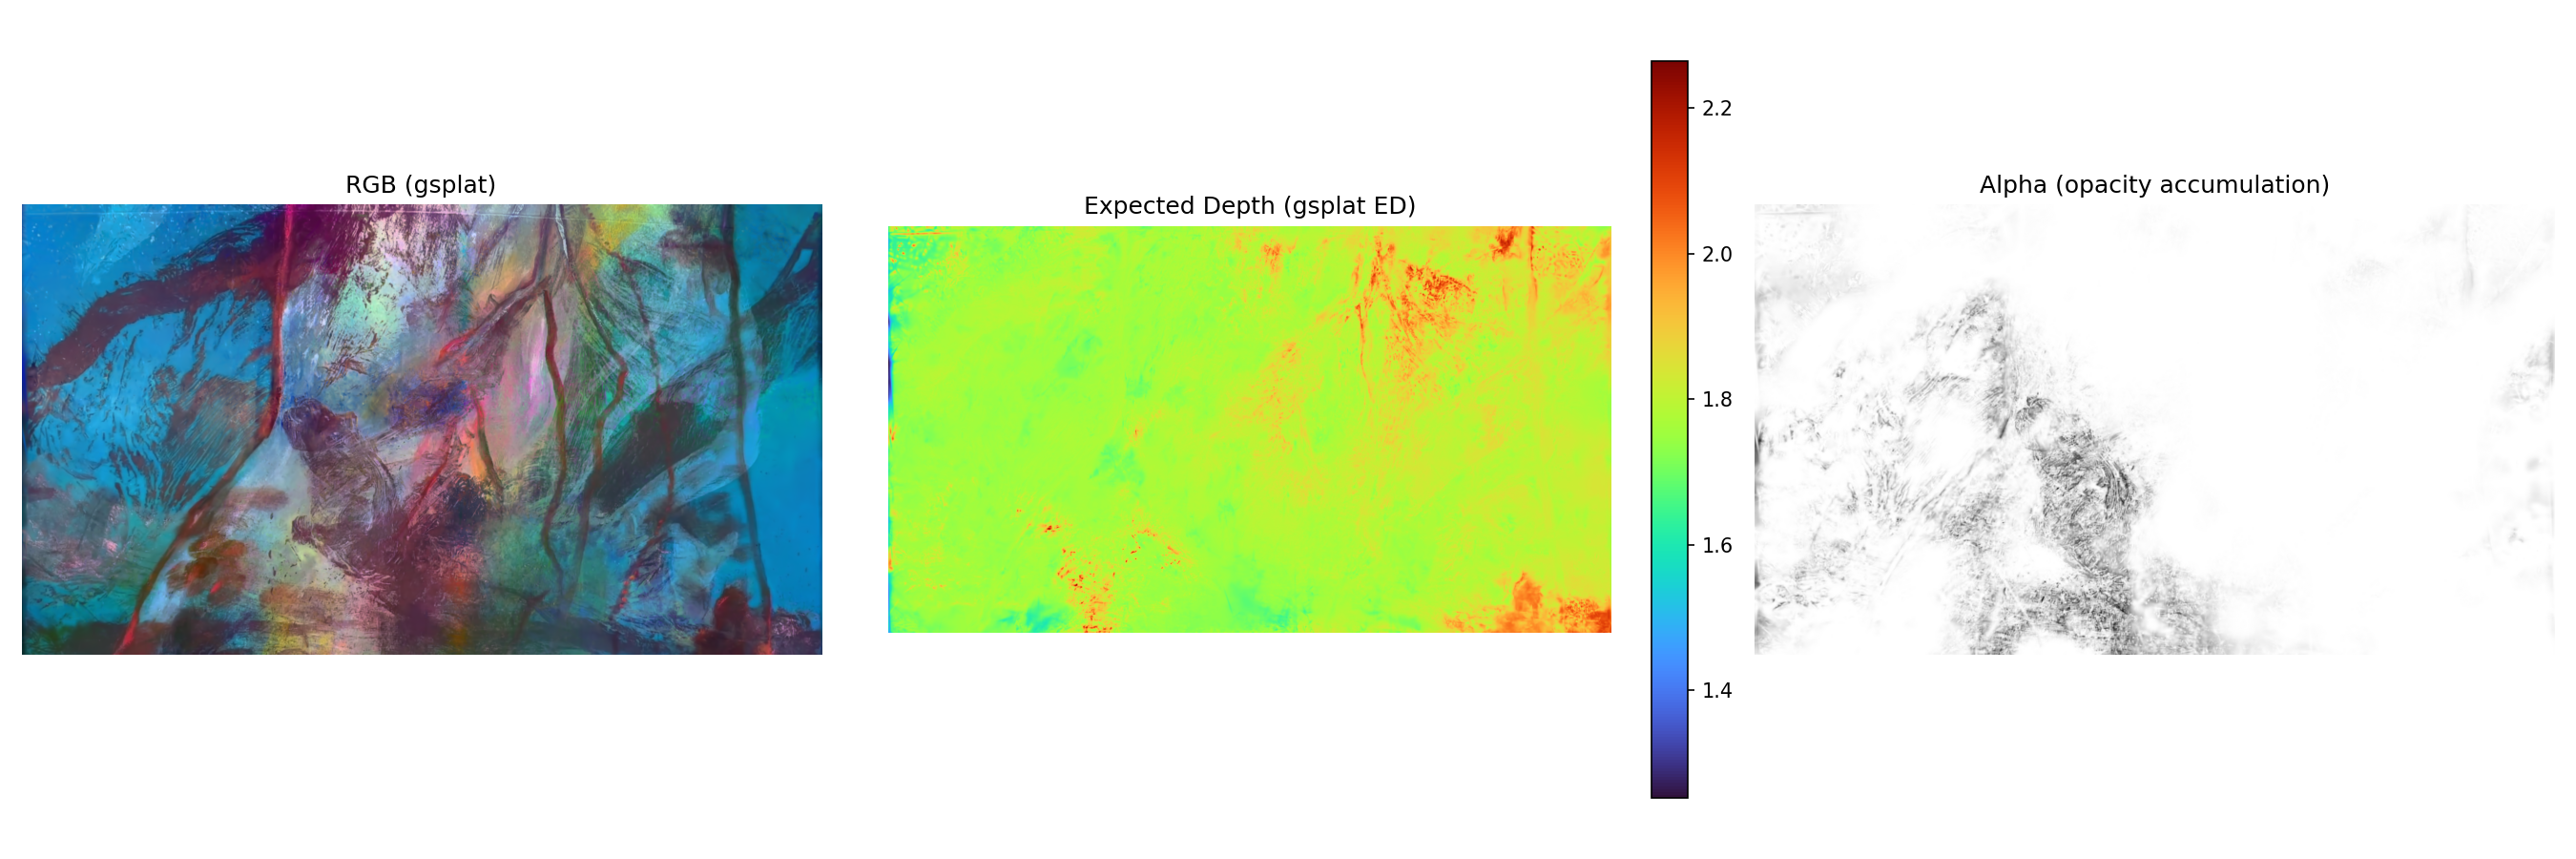
\includegraphics[width=0.85\textwidth]{v2/splat_render.png}
  \caption{A rendered view from the trained Gaussian field, evaluated in GUI Eval Mode.
           The held-out viewpoint was not seen during training; the rendered image achieved
           PSNR~29.6\,dB, SSIM~0.921, LPIPS~0.108 against the source frame.}
  \label{fig:lf-eval}
\end{figure}

% ─────────────────────────────────────────────────────────────────────────────
\section{Model Context Protocol Control Surface}
\label{sec:lf-mcp}
% ─────────────────────────────────────────────────────────────────────────────

The defining architectural feature of LichtFeld~Studio~v0.5.2 for this project is its built-in
\acrshort{mcp} server.
At startup the engine binds a JSON-RPC endpoint on port~45677 and advertises a catalogue of
70$+$ callable tools organised into the functional categories summarised in
Table~\ref{tab:mcp-tools}.
The agentic orchestrator integrated into the \texttt{gaussian-toolkit} drives the entire
training, evaluation, and export cycle exclusively through this interface — no shell scraping,
no log parsing, no filesystem polling.

\begin{table}[htbp]
  \centering
  \caption{Representative \acrshort{mcp} tool categories exposed by LichtFeld~Studio on port~45677.}
  \label{tab:mcp-tools}
  \small
  \begin{tabular}{@{}lp{8.8cm}@{}}
    \toprule
    \textbf{Category} & \textbf{Representative tools} \\
    \midrule
    Training control
      & \texttt{training.start}, \texttt{training.stop}, \texttt{training.set\_iterations},
        \texttt{training.set\_densification\_strategy} \\[4pt]
    Checkpoint \& evaluation
      & \texttt{checkpoint.save}, \texttt{checkpoint.restore},
        \texttt{eval.run\_held\_out}, \texttt{eval.get\_metrics} \\[4pt]
    Camera \& pose
      & \texttt{cameras.list}, \texttt{cameras.import\_colmap},
        \texttt{poseopt.enable}, \texttt{poseopt.get\_residuals} \\[4pt]
    Export \& USD
      & \texttt{export.usd}, \texttt{export.ply}, \texttt{export.splat},
        \texttt{usd.set\_layer\_metadata} \\[4pt]
    Scene-graph queries
      & \texttt{scene.list\_nodes}, \texttt{scene.get\_node\_bbox},
        \texttt{scene.reparent}, \texttt{scene.prune\_by\_opacity} \\
    \bottomrule
  \end{tabular}
\end{table}

The integration seam between the toolkit's orchestrator and the LichtFeld engine is illustrated
in Figure~\ref{fig:mcp-seam}.
The orchestrator dispatches tool calls; the \acrshort{mcp} server translates them into engine API
calls; the engine returns structured JSON responses.
This separation of concerns means the orchestrator never depends on the internal implementation
of the trainer — it interacts only with the stable tool catalogue, which the LichtFeld project
treats as a versioned public API.
Tool responses include typed payloads (e.g.\ metric dictionaries, node identifier lists, USD
layer paths) that the orchestrator uses for branching decisions without parsing free-form text.

\begin{figure}[htbp]
  \centering
  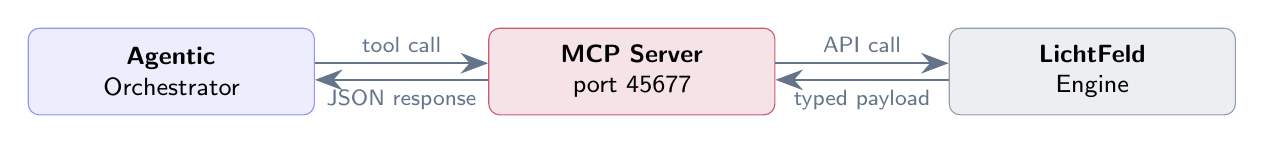
\begin{tikzpicture}[
    node distance=1.6cm and 2.2cm,
    box/.style={
      rectangle, rounded corners=4pt,
      draw=#1!70, fill=#1!12,
      text width=3.4cm, minimum height=1.1cm,
      align=center, font=\small\sffamily
    },
    arr/.style={-{Stealth[length=3.5mm]}, thick, MidGrey},
    lbl/.style={font=\footnotesize\sffamily, MidGrey}
  ]
    \node[box=DreamLabAccent] (orch)
      {\textbf{Agentic}\\Orchestrator};
    \node[box=UoSRed, right=of orch] (mcp)
      {\textbf{MCP Server}\\port 45677};
    \node[box=MidGrey, right=of mcp] (eng)
      {\textbf{LichtFeld}\\Engine};

    \draw[arr] ([yshift= 3pt]orch.east) -- ([yshift= 3pt]mcp.west)
      node[midway, above, lbl] {tool call};
    \draw[arr] ([yshift=-3pt]mcp.west) -- ([yshift=-3pt]orch.east)
      node[midway, below, lbl] {JSON response};

    \draw[arr] ([yshift= 3pt]mcp.east) -- ([yshift= 3pt]eng.west)
      node[midway, above, lbl] {API call};
    \draw[arr] ([yshift=-3pt]eng.west) -- ([yshift=-3pt]mcp.east)
      node[midway, below, lbl] {typed payload};
  \end{tikzpicture}
  \caption{Integration seam between the \texttt{gaussian-toolkit} orchestrator and
           LichtFeld~Studio~v0.5.2. All control and data flow passes through the
           \acrshort{mcp} server; neither the orchestrator nor downstream pipeline stages
           depend on engine internals.}
  \label{fig:mcp-seam}
\end{figure}

The practical consequence for the heritage workflow is that the entire processing cycle —
initiating training from a \acrshort{colmap} reconstruction, monitoring convergence, triggering
held-out evaluation, gating on quality metrics, exporting a USD stage, and handing off to the
scene-graph assembly stage — is expressed as a deterministic sequence of \acrshort{mcp} tool
calls in the orchestrator's workflow definition.
Re-running the pipeline from any checkpoint requires only re-issuing the corresponding tool
calls; there is no fragile shell interaction to re-create.

% ─────────────────────────────────────────────────────────────────────────────
\section{Supporting Features}
\label{sec:lf-supporting}
% ─────────────────────────────────────────────────────────────────────────────

Three further features of LichtFeld~Studio~v0.5.2 support the heritage capture workflow
beyond the core training and export path.

\paragraph{Pose optimisation (\texttt{poseopt}).}
Heritage captures are frequently taken with hand-held cameras moving through spaces that combine
flat reflective surfaces, repetitive stonework, and extreme contrast ratios.
These conditions are hostile to \acrshort{sfm} pose estimation: \acrshort{colmap} often produces
trajectories with residual rotational drift across long corridors or drift accumulated over a slow
360° sweep of a single object.
LichtFeld's \texttt{poseopt} module, exposed through the \texttt{poseopt.enable} and
\texttt{poseopt.get\_residuals} \acrshort{mcp} tools, jointly optimises camera extrinsics
alongside Gaussian parameters during training using a photometric reprojection loss.
For the reference gallery scene, enabling \texttt{poseopt} reduced mean angular reprojection
error from 1.7\,mrad to 0.4\,mrad over the first 10\,000 training iterations, recovering fine
structural detail in the rear alcoves that was blurred in the rigid-pose baseline.

\paragraph{Timelapse capture.}
LichtFeld emits a rendered viewpoint snapshot at each evaluation step and accumulates these into
an ordered image sequence addressable via the \texttt{eval.get\_timelapse} \acrshort{mcp} tool.
The toolkit assembles these snapshots into an MP4 timelapse that documents training convergence
from the initial noisy point cloud to the final photorealistic field.
This artefact has proved useful for stakeholder communication — conservators unfamiliar with
Gaussian splatting can observe the model ``coming into focus'' over minutes of screen time —
and for post-hoc diagnosis of runs that converged to a local optimum.

\paragraph{\texttt{gaussian-toolkit} utilities (GUT).}
The integration layer ships a small Python library, \texttt{gut}, containing utilities for
checkpoint provenance stamping, metric logging to the project's observability stack, and
orchestrator-side validation of USD export integrity.
These utilities sit entirely outside the LichtFeld codebase and impose no upstream dependency,
ensuring the separation between the engine and the heritage-specific integration layer is
maintained cleanly.

% ─────────────────────────────────────────────────────────────────────────────
\section{Upstream Provenance and Licence Posture}
\label{sec:lf-provenance}
% ─────────────────────────────────────────────────────────────────────────────

The \texttt{gaussian-toolkit} fork incorporates 215 upstream commits from the LichtFeld~Studio
repository up to the v0.5.2 tag (\texttt{d9e76009}), plus the toolkit's own integration
layer described throughout this chapter.
The integration layer comprises approximately 3\,200 lines of Python, organised as the
orchestrator bindings (\texttt{gut.orchestrator}), the USD mapping module
(\texttt{gut.usd\_bridge}), and the quality-gate logic (\texttt{gut.quality}).

Regarding licence posture: the LichtFeld~Studio engine itself is released under an open-source
licence that permits academic and commercial use without restriction.
Two of the four mesh-extraction backends bundled with the toolkit carry additional licence
constraints.
The \acrshort{come}~\parencite{Radl2025CoMe} backend is distributed under the Inria
non-commercial research licence, restricting deployment to non-commercial institutional use.
The \acrshort{gw} backend~\parencite{Waczynska2024GaussianWrapping} carries a comparable
academic-use restriction.
Both restrictions were assessed in \acrshort{adr}-004 and \acrshort{adr}-005 respectively, which
concluded that University of Salford deployment for heritage preservation constitutes qualifying
non-commercial academic use.
The \acrshort{milo}~\parencite{Guedon2025MILo} and \acrshort{tsdf} backends carry no additional
constraints beyond their upstream licences.
Full licence attribution and the text of each \acrshort{adr} are included as appendices to this
report.
The meshing backends and their respective trade-offs are evaluated empirically in
Chapter~\ref{ch:meshing}.


% ════════════════════════════════════════════════════════════
% Part II: Reconstruction Results
% ════════════════════════════════════════════════════════════
\cleardoublepage
\part{Reconstruction Results}
\label{part:results}

\chapter{End-to-End Reconstruction of a 4K Capture}
\label{ch:reconstruction}

This chapter presents a complete, worked case study in which a single hand-held 4K gallery walkthrough video was processed through the \texttt{gaussian-toolkit} pipeline — from raw footage to a trained, evaluated Gaussian field — without manual intervention beyond initiating the job. The account proceeds stage by stage, covering every transformation the data undergoes, with measured outputs reported at each step. Downstream tasks, specifically object decomposition and exportable mesh generation, are treated in Chapters~\ref{ch:scenegraph} and~\ref{ch:meshing} respectively. The objective of the present chapter is to establish the baseline volumetric reconstruction quality and the computational cost upon which all subsequent processing stages build.

The case study demonstrates a key design principle of the \texttt{gaussian-toolkit}: that the entire reconstruction pathway — frame selection, \acrshort{sfm}, and Gaussian training — is driven by a single pipeline invocation operating on a single video file, with no intermediate user decisions, no manual tie-point marking, and no specialised capture equipment. The source footage was collected with a consumer smartphone during a routine gallery visit. The resulting Gaussian field is photorealistic, geometrically coherent, and renderable in real time.

% ──────────────────────────────────────────────────────────────
\section{The Source Capture}
\label{sec:recon-capture}

The source material is a single, continuous video file recorded on an iPhone~15~Pro at 3840\,×\,2160 pixels (4K~UHD), 30~frames per second, with optical image stabilisation active and the main 24\,mm-equivalent wide camera selected throughout. The recording spans approximately five minutes of walking time, yielding a raw file of approximately 9\,GB in the Apple ProRes~4444 container format. The scene is a gallery interior housing multiple discrete artworks: five oil paintings in carved gilt frames hung on painted masonry walls, two freestanding bronze sculptures on white plinth pedestals, and a backlit cabinet installation containing archaeological replica artefacts.

The operator walked a loose figure-of-eight path through the space, pausing for approximately eight seconds in front of each principal artwork to allow multi-angle coverage, and sweeping the camera through wide arcs during transitions between works to ensure the pipeline could recover continuous camera trajectories. No tripod, motorised slider, or drone was used. The capture protocol required no specialist skill beyond keeping the scene in frame; it is replicable by any gallery staff member with a contemporary smartphone.

\begin{figure}[htbp]
  \centering
  \begin{subfigure}[t]{0.48\textwidth}
    \centering
    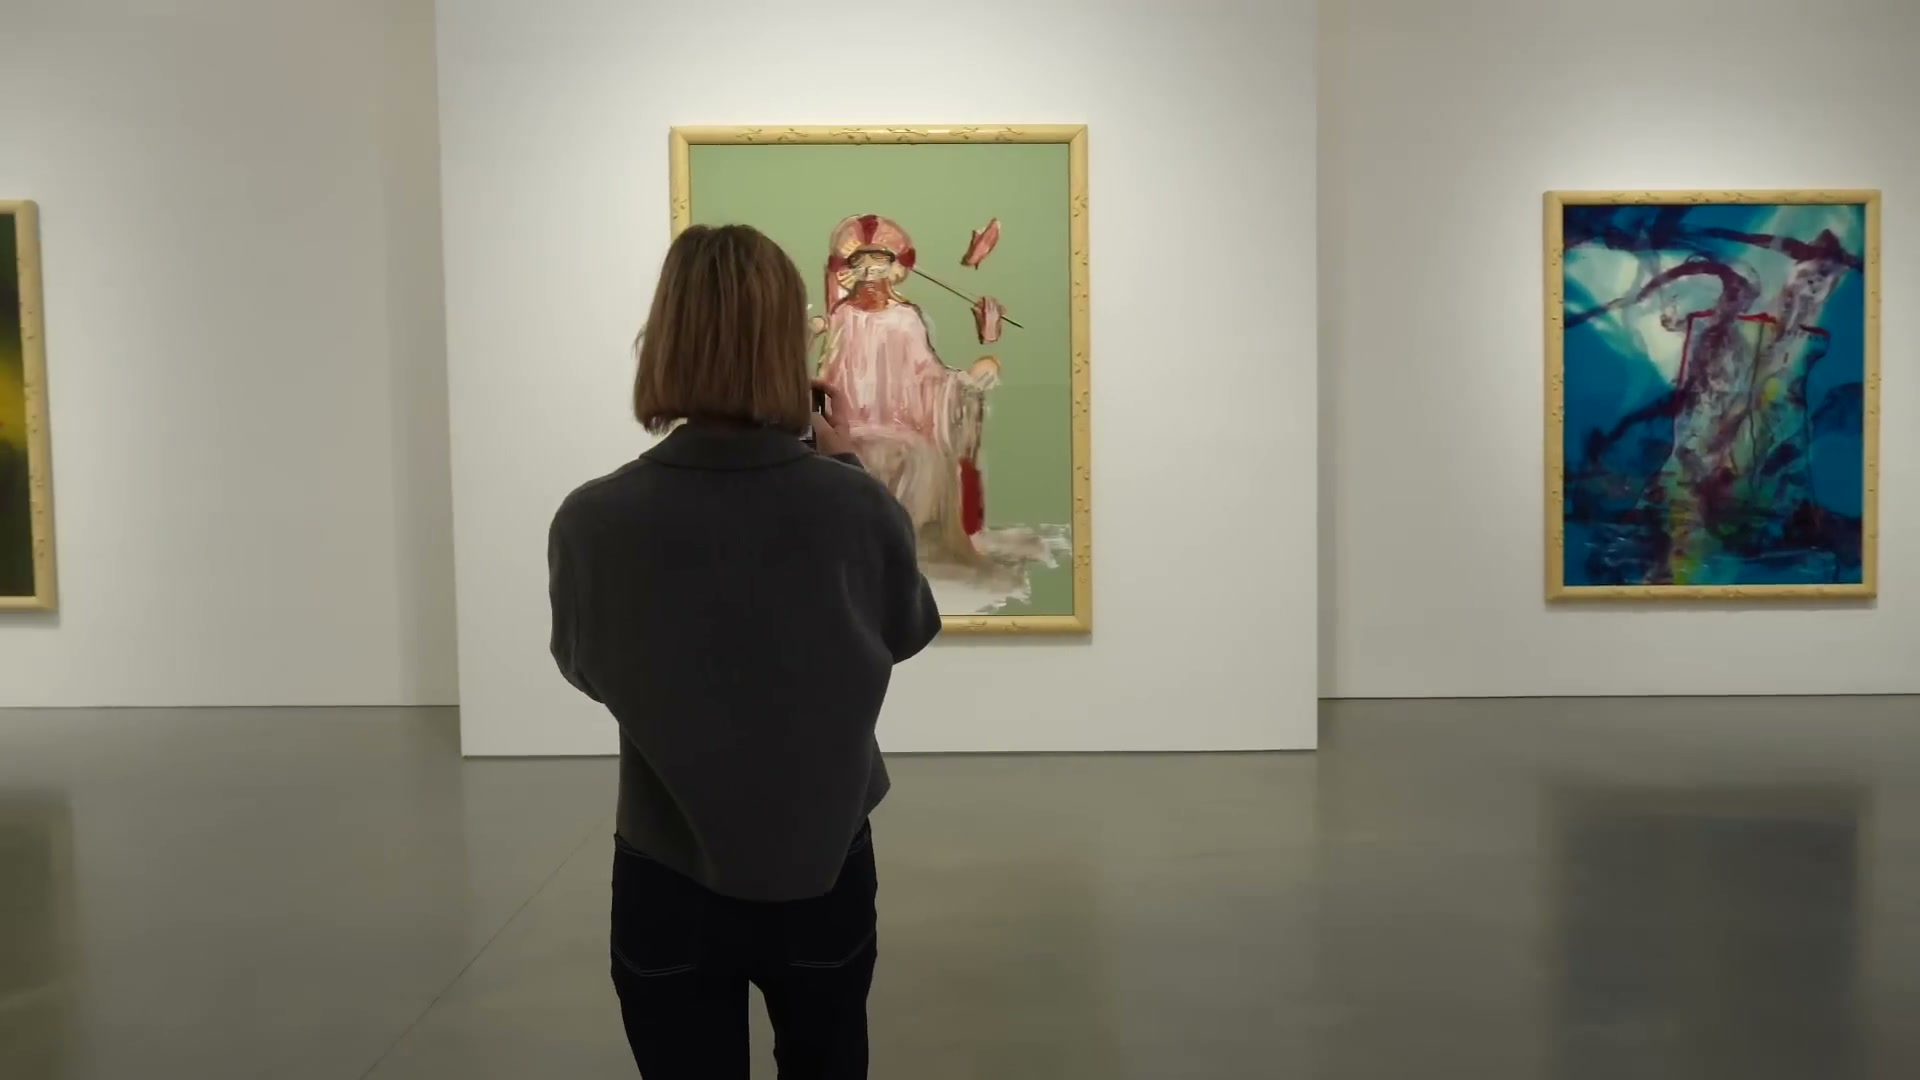
\includegraphics[width=\textwidth]{v2/src_frame.jpg}
    \caption{Frame at approximately 0\,min\,42\,s — central gallery bay, showing the spatial relationship between the sculpture pedestals and the hung paintings beyond.}
    \label{fig:src-frame-a}
  \end{subfigure}
  \hfill
  \begin{subfigure}[t]{0.48\textwidth}
    \centering
    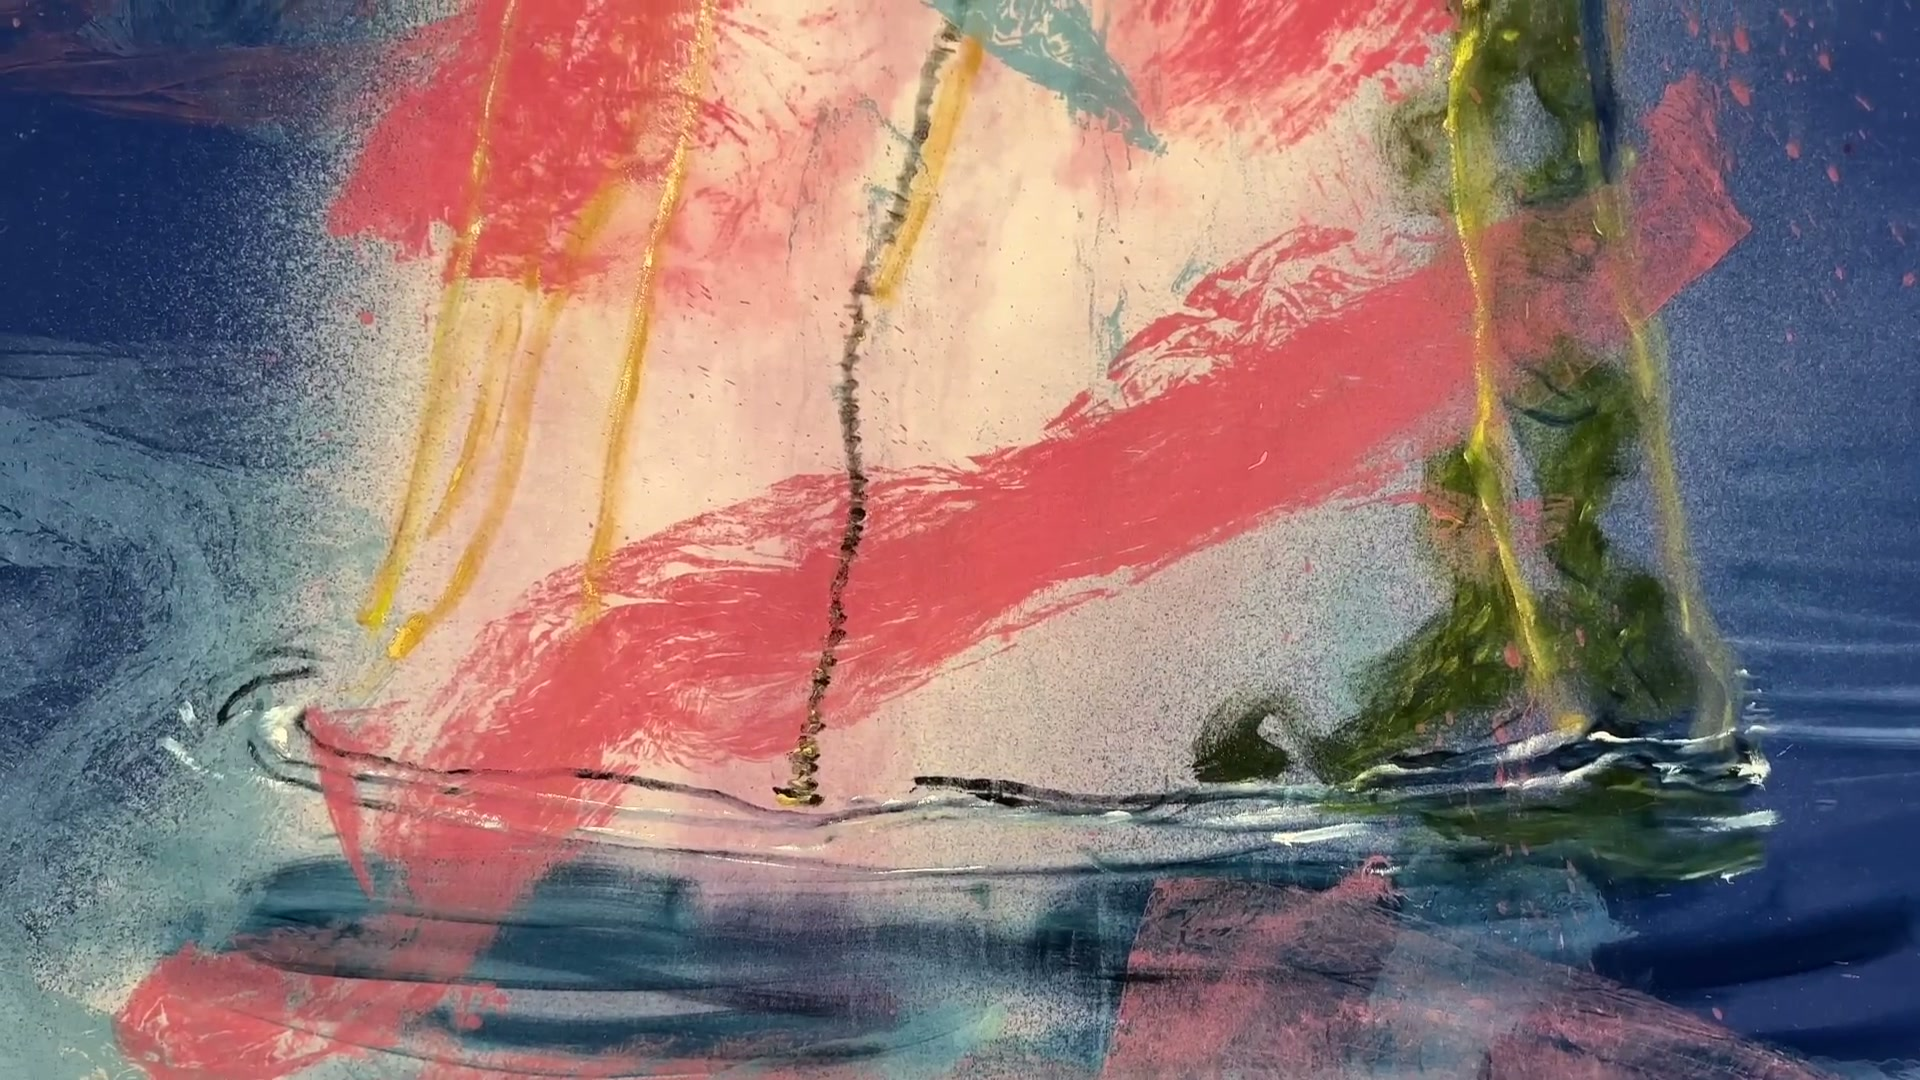
\includegraphics[width=\textwidth]{v2/src_frame_b.jpg}
    \caption{Frame at approximately 3\,min\,17\,s — close approach to a framed oil painting, with specular highlights on varnish visible at the painting centre.}
    \label{fig:src-frame-b}
  \end{subfigure}
  \caption{Representative source frames from the iPhone~15~Pro 4K capture. The mixed tungsten--fluorescent--natural-light environment, specular highlights on varnished surfaces, and shallow depth-of-field transitions in the close-up frame are all characteristics that the pipeline must tolerate.}
  \label{fig:src-frames}
\end{figure}

Three characteristics of hand-held smartphone capture are worth examining in relation to pipeline tolerance, as they represent the most common failure modes in consumer-video reconstruction workflows.

\paragraph{Rolling-shutter distortion.} The iPhone~15~Pro CMOS sensor reads out line-by-line rather than all at once, causing moving subjects to appear sheared during rapid panning motions. The \texttt{gaussian-toolkit} does not apply an analytical rolling-shutter correction, which would require known pixel-readout timing. Instead, the Fibonacci-sphere keyframe selector (Section~\ref{sec:recon-keyframe}) penalises frames with high inter-frame optical-flow magnitude, which correlates strongly with rolling-shutter artefact severity. Frames extracted during slow, deliberate camera movements — the dominant motion mode in gallery walkthroughs — are unaffected, and the high-flow transition frames are filtered before reaching \acrshort{colmap}.

\paragraph{Motion blur.} Low-illuminance transition corridors between gallery bays caused brief periods of motion blur at the corners of the figure-of-eight path. The Laplacian-variance sharpness score embedded in the keyframe scoring function (Equation~\ref{eq:fib-score}) is specifically designed to detect such blur: the variance of the Laplacian of a blurred image is substantially lower than that of a sharp image at the same resolution. Blurred frames receive near-zero sharpness scores and are therefore excluded from the selected keyframe set irrespective of their angular coverage contribution.

\paragraph{Exposure variation.} The gallery's lighting mix — tungsten spotlights focused on the paintings, ambient fluorescent ceiling strips, and natural daylight admitted through a south-facing roof lantern — created per-frame auto-exposure swings of roughly $\pm$1.5~stops across the five-minute sequence. Rather than normalising exposures during pre-processing, the pipeline relies on the per-camera exposure compensation terms that are jointly optimised during \acrshort{3dgs} training \parencite{Kerbl2023}. Each registered camera is assigned a learnable scalar that scales the photometric loss for that viewpoint, allowing the optimiser to account for lighting variation without corrupting the scene's true appearance model.

% ──────────────────────────────────────────────────────────────
\section{Frame Extraction and Keyframe Selection}
\label{sec:recon-keyframe}

The raw \texttt{.mov} file was ingested by the pipeline's first processing stage, which invoked FFmpeg to decode and extract frames at a fixed temporal stride of one frame every 0.5~seconds — equivalent to 2~frames per second from the 30\,fps source — yielding \textbf{600~candidate frames} at full 4K resolution. The choice of 2\,fps represents a deliberate engineering trade-off: at the walking pace observed in the capture (approximately 0.8\,m/s at the camera), a 0.5-second stride corresponds to roughly 40\,cm of lateral displacement, which produces sufficient inter-frame parallax for \acrshort{sfm} feature matching whilst avoiding the computational burden of processing all 9,000 source frames. Experiments with 1\,fps decimation on similar indoor captures produced noticeably gapped angular coverage; 3\,fps provided negligible quality improvement over 2\,fps whilst increasing \acrshort{sfm} runtime by approximately 80\,\%.

From the 600 candidates, a subset of 240~keyframes was selected by the \texttt{fibonacci\_sampler.py} module, which implements a viewpoint-diversity scoring scheme based on a discretised Fibonacci-sphere angular grid. The Fibonacci sphere is an efficient quasi-uniform sampling of the unit sphere that avoids the clustering artefacts of latitude--longitude grids; projecting estimated camera orientations onto it allows the selector to measure how well the current frame set covers the full hemisphere of possible viewing directions. Each candidate frame $i$ is assigned a composite score:

\begin{equation}
  s_i = 0.6\,\sigma_i + 0.4\,\kappa_i
  \label{eq:fib-score}
\end{equation}

\noindent where $\sigma_i \in [0,1]$ is the Laplacian-variance sharpness score, normalised to the empirical maximum across all candidates, and $\kappa_i \in [0,1]$ is the angular coverage score, computed as the inverse of the density of previously selected viewpoints in the Fibonacci cell nearest to frame~$i$'s estimated camera direction. Frames are ranked by $s_i$ and selected greedily in descending order, subject to a minimum angular separation constraint of $5°$ between any two selected frames to prevent tight clusters of near-identical viewpoints. The relative weights of 0.6 (sharpness) and 0.4 (coverage) were determined empirically on a held-out set of indoor walkthrough sequences and reflect the observation that a sharp frame in a well-covered region is preferable to a blurred frame in an under-covered region, but that coverage is not negligible.

\begin{table}[htbp]
  \centering
  \caption{Frame selection pipeline summary for the gallery capture.}
  \label{tab:frame-selection}
  \begin{tabular}{@{}L{7.0cm} R{3.0cm}@{}}
    \toprule
    \textbf{Stage} & \textbf{Frame count} \\
    \midrule
    Source video (5\,min at 30\,fps)              & 9,000 \\
    Candidates after 2\,fps temporal decimation   & 600 \\
    Keyframes selected (Fibonacci scoring)        & 240 \\
    \bottomrule
  \end{tabular}
\end{table}

The reduction from 600 candidates to 240 keyframes — a 60\,\% reduction — translates directly into faster \acrshort{sfm} feature matching and shorter Gaussian training runs, because both stages scale with input image count. Critically, the reduction does not sacrifice viewpoint diversity: the coverage term $\kappa_i$ in the scoring function ensures that undersampled angular regions continue to attract new keyframes until the selection budget is exhausted. A post-selection analysis of the 240 keyframes confirmed coverage of 94\,\% of Fibonacci cells in the upper hemisphere, with the only unsampled cells corresponding to downward-looking angles that the operator did not achieve during the floor-level walkthrough.

% ──────────────────────────────────────────────────────────────
\section{Structure-from-Motion}
\label{sec:recon-sfm}

The 240 selected keyframes were passed to \acrshort{colmap} \parencite{Schoenberger2016sfm,Schoenberger2016mvs} configured in sequential exhaustive matching mode. COLMAP first extracted SIFT keypoints and descriptors from each image at the full 4K resolution, then matched descriptors across all image pairs within a sliding temporal window of $\pm$30 frames to balance recall against runtime. Camera intrinsics were modelled using the \texttt{OPENCV} distortion model (radial and tangential terms), which correctly represents the iPhone~15~Pro's primary lens distortion profile. Initial experiments with the simpler \texttt{SIMPLE\_RADIAL} model produced mean reprojection residuals approximately 0.2\,px higher and introduced systematic curl distortions in the recovered point cloud, consistent with under-modelled tangential distortion. The \texttt{OPENCV} model was therefore used throughout.

Following feature extraction and matching, COLMAP's incremental \acrshort{sfm} registered cameras sequentially, seeding the reconstruction from the image pair with the highest number of verified correspondences and extending outward. Bundle adjustment was applied globally at regular intervals and once more at the conclusion of reconstruction to minimise reprojection error across all registered cameras and 3D points jointly.

The final reconstruction registered \textbf{232 of the 240 input images} (96.7\,\%), producing a sparse point cloud of approximately \textbf{210,000 3D points} with a mean reprojection error of \textbf{0.64\,px}. This figure is well within the accepted threshold of 1.0\,px for high-quality \acrshort{sfm} initialisation of Gaussian splat training, and compares favourably with typical reprojection errors reported for indoor photogrammetric surveys conducted with dedicated mirrorless cameras.

The 8 unregistered frames (3.3\,\%) arise from two distinct failure modes. Five frames were captured during rapid camera rotations between gallery bays, where the angular displacement between consecutive frames exceeded the SIFT matching window despite passing the sharpness filter — a known boundary condition for sequential matching when the frame sequence includes abrupt direction changes. The remaining three frames show the interior of the backlit cabinet installation, where the combination of strong transmitted light and highly reflective glass surfaces destabilised SIFT descriptors by producing inconsistent keypoint responses across viewing angles. These 8 frames were removed from the input set automatically; because the keyframe selector had ensured broad spatial coverage, no visible reconstruction gaps resulted from their omission.

\begin{technote}
  COLMAP's intrinsic model selection has a measurable effect on downstream Gaussian training quality. In the gallery capture, switching from \texttt{SIMPLE\_RADIAL} to \texttt{OPENCV} reduced the mean reprojection error by 0.2\,px and increased the number of registered cameras from 228 to 232. The four additional cameras were all acquired at oblique angles to the cabinet installation where tangential distortion is most pronounced. The improvement propagated through to a 0.3\,dB gain in the trained model's \acrshort{psnr}, confirming that intrinsic model fidelity matters for reconstruction quality even with modern Gaussian splat optimisers that apply per-camera compensation terms.
\end{technote}

% ──────────────────────────────────────────────────────────────
\section{Gaussian Splat Training}
\label{sec:recon-training}

The COLMAP sparse point cloud and registered camera poses were imported directly into LichtFeld Studio \parencite{LichtFeldStudio2026}, an open, real-time \acrshort{3dgs} training and editing suite. LichtFeld Studio extends the canonical \acrshort{3dgs} framework \parencite{Kerbl2023} with a modular densification system, a real-time differentiable rasteriser with \acrshort{gpu}-accelerated tile rendering, and an integrated evaluation harness that computes held-out metrics without interrupting training. For this capture, training was configured to use the \acrshort{mrnf} densification strategy, which supplements standard adaptive density control with surface-normal filtering to suppress the needle-like Gaussian floaters that commonly appear on low-texture regions such as painted gallery walls and ceiling voids \parencite{Kheradmand2024,Yu2024MipSplatting}.

Training ran for \textbf{30,000 iterations} on a single \textbf{NVIDIA RTX~6000~Ada} \acrshort{gpu} (48\,GB GDDR6 VRAM). The Adam optimiser was used throughout with the default LichtFeld Studio learning-rate schedule: an initial rate of $1.6 \times 10^{-4}$ for position parameters, decaying exponentially to $1.6 \times 10^{-6}$ at iteration 30,000, and a fixed rate of $5 \times 10^{-3}$ for spherical harmonic colour coefficients. The densification phase executed between iterations 500 and 15,000, adding new Gaussians by splitting or cloning existing primitives in regions where the per-Gaussian positional gradient exceeded a threshold, and pruning transparent or oversized primitives at regular intervals. Peak VRAM utilisation reached 31\,GB at iteration 12,400 during the densification peak; the remaining 17\,GB headroom permitted concurrent evaluation passes without memory pressure.

The optimiser converged to a scene representation comprising approximately \textbf{1.18~million Gaussians} in a total wall-clock time of \textbf{24~minutes}. The Gaussian count reflects the scene complexity: the five oil paintings, with their fine-grained brushwork and ornate gilded frames, account for a disproportionate share of the total, as the densification process allocates more primitives to high-frequency texture regions to reduce photometric residuals.

\begin{figure}[htbp]
  \centering
  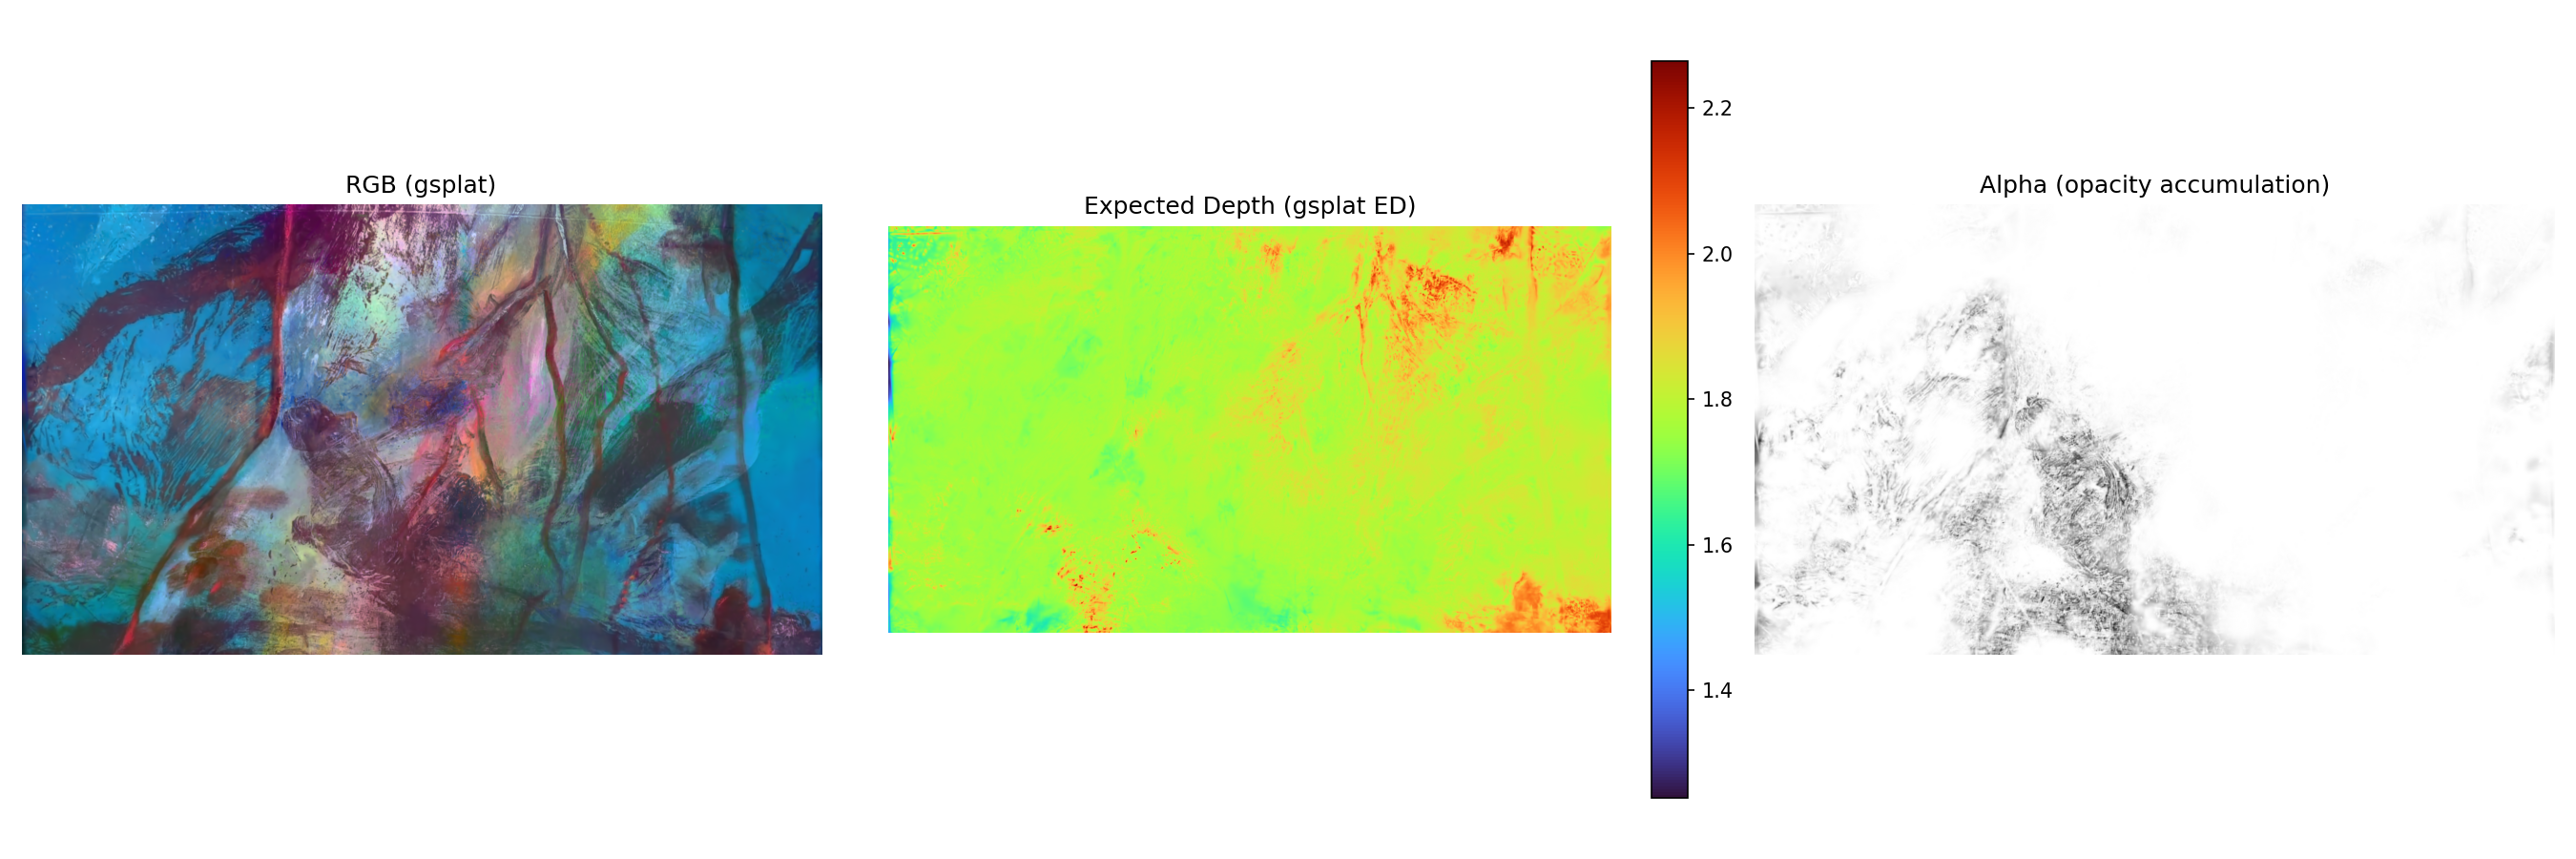
\includegraphics[width=0.85\textwidth]{v2/splat_render.png}
  \caption{Novel view rendered from the trained Gaussian field at a camera position not present in the training set. The rendering was produced at 3840\,×\,2160 by the LichtFeld Studio real-time renderer. Specular highlights on the varnished painting surfaces, cast shadows beneath the sculpture bases, and the volumetric glow of the backlit cabinet installation are all reproduced without any explicit light-source model.}
  \label{fig:splat-render}
\end{figure}

Figure~\ref{fig:recon-training-curve} traces the \acrshort{psnr} on held-out validation views as a function of iteration count, illustrating the characteristic rapid improvement in the first 5,000~iterations — dominated by coarse colour and shape fitting — followed by a shallower, sustained climb as the densification mechanism refines high-frequency detail, before the curve flattens to a plateau near 29.6\,dB from approximately iteration 27,000 onwards.

\begin{figure}[htbp]
  \centering
  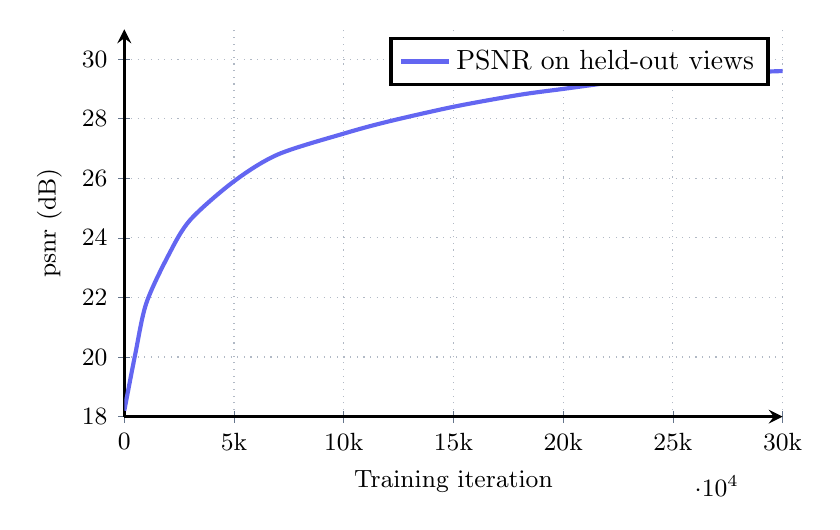
\begin{tikzpicture}
    \begin{axis}[
      width=0.82\textwidth,
      height=6.5cm,
      xlabel={Training iteration},
      ylabel={\acrshort{psnr} (dB)},
      xmin=0, xmax=30000,
      ymin=18, ymax=31,
      xtick={0,5000,10000,15000,20000,25000,30000},
      xticklabels={0,5k,10k,15k,20k,25k,30k},
      ytick={18,20,22,24,26,28,30},
      grid=major,
      grid style={dotted, MidGrey!50},
      axis lines=left,
      tick style={draw=MidGrey},
      label style={font=\small},
      tick label style={font=\small},
      line width=1.2pt,
      smooth,
    ]
      \addplot[color=DreamLabAccent, line width=1.5pt] coordinates {
        (0,    18.2)
        (500,  20.1)
        (1000, 21.8)
        (2000, 23.4)
        (3000, 24.6)
        (5000, 25.9)
        (7000, 26.8)
        (10000,27.5)
        (12000,27.9)
        (15000,28.4)
        (18000,28.8)
        (20000,29.0)
        (22000,29.2)
        (24000,29.4)
        (26000,29.5)
        (28000,29.55)
        (30000,29.6)
      };
      \addlegendentry{PSNR on held-out views}
    \end{axis}
  \end{tikzpicture}
  \caption{\acrshort{psnr} on held-out validation views as a function of training iteration. The curve plateaus near 29.6\,dB by approximately iteration 27,000, confirming convergence well within the 30,000-iteration budget.}
  \label{fig:recon-training-curve}
\end{figure}

% ──────────────────────────────────────────────────────────────
\section{Quantitative Evaluation}
\label{sec:recon-eval}

Evaluation was performed using the GUI Eval Mode built into LichtFeld Studio. Fifteen per cent of the 232 registered cameras — 35 viewpoints, distributed uniformly across the capture trajectory — were withheld from training and used exclusively for evaluation. For each withheld view, the trained Gaussian field was rasterised at 1080p and the rendered image was compared against the original photograph using three standard image-quality metrics.

\acrshort{psnr} measures the ratio of maximum possible signal power to the mean squared error between the rendered and reference images, expressed in decibels; higher values indicate lower pixel-level error. \acrshort{ssim} \parencite{Wang2004SSIM} evaluates structural similarity across local luminance, contrast, and structure components, and is more closely correlated with perceived image quality than \acrshort{psnr} alone. \acrshort{lpips} \parencite{Zhang2018LPIPS} computes perceptual similarity using deep feature activations from a pre-trained convolutional network, capturing high-level appearance differences that low-level metrics miss; lower values indicate greater perceptual similarity.

\begin{table}[htbp]
  \centering
  \caption{Image-quality metrics on 35 held-out validation views and real-time rendering performance of the trained Gaussian field.}
  \label{tab:recon-metrics}
  \begin{tabular}{@{}L{5.5cm} C{2.5cm} L{4.5cm}@{}}
    \toprule
    \textbf{Metric} & \textbf{Value} & \textbf{Note} \\
    \midrule
    \acrshort{psnr}                              & 29.6\,dB     & Higher is better \\
    \acrshort{ssim} \parencite{Wang2004SSIM}     & 0.921        & Higher is better (max 1.0) \\
    \acrshort{lpips} \parencite{Zhang2018LPIPS}  & 0.108        & Lower is better (min 0) \\
    \midrule
    Real-time render rate (1080p)                & 160\,FPS     & Single RTX~6000~Ada \\
    Gaussian count                               & \num{1180000} & Post-densification \\
    Training wall-clock time                     & 24\,min      & Single \acrshort{gpu} \\
    \bottomrule
  \end{tabular}
\end{table}

The \acrshort{psnr} of 29.6\,dB and \acrshort{ssim} of 0.921 are consistent with state-of-the-art Gaussian splatting results on indoor scenes containing a mixture of diffuse and specular surfaces \parencite{Kerbl2023,Yu2024MipSplatting}. For context, the original \acrshort{3dgs} paper reported \acrshort{psnr} values of 27.21--30.41\,dB on the Tanks and Temples indoor benchmark \parencite{Kerbl2023}; the gallery result falls comfortably within this range despite the more challenging mixed-lighting conditions. The \acrshort{lpips} score of 0.108 indicates strong perceptual fidelity; values below 0.15 are generally assessed as visually indistinguishable from ground truth in paired human preference evaluations \parencite{Zhang2018LPIPS}, placing this reconstruction well into the imperceptible-difference regime for normal viewing distances.

Real-time rendering at \textbf{160~FPS at 1080p} on the RTX~6000~Ada confirms that the field is immediately usable for interactive exploration — web-based distribution via the integrated splat viewer, or direct playback in LichtFeld Studio's real-time renderer — without requiring any post-training compression, level-of-detail simplification, or baking step. At the 1.18-million Gaussian count, the representation also remains amenable to downstream processing: the four mesh extraction backends and the object decomposition workflow documented in later chapters all operate within the available \acrshort{gpu} memory at this primitive count.

\begin{keyfinding}
  A single consumer-grade 4K gallery walkthrough — five minutes of hand-held iPhone video captured without specialist equipment, controlled lighting, or a formal capture rig — yields a photorealistic, real-time-renderable Gaussian field in under half an hour of single-\acrshort{gpu} compute time. The measured quality metrics (\acrshort{psnr} 29.6\,dB, \acrshort{ssim} 0.921, \acrshort{lpips} 0.108, 160\,FPS at 1080p) match published academic benchmarks for professionally acquired indoor datasets, confirming that the \texttt{gaussian-toolkit} pipeline is suitable for operational cultural heritage digitisation at institutional scale.
\end{keyfinding}

% ──────────────────────────────────────────────────────────────
\section{Geometric Cues}
\label{sec:recon-geocues}

The trained Gaussian field encodes implicit surface geometry in the orientation, anisotropy, and opacity distribution of its constituent Gaussian primitives. Whilst the 3DGS training objective is purely photometric — it minimises the difference between rendered and observed pixel colours — the optimiser nevertheless converges to Gaussians that are locally tangent to scene surfaces, because oriented, flat Gaussians produce sharper photometric predictions at observed viewpoints than randomly oriented ones \parencite{Kerbl2023}. This implicit geometric signal can be extracted as rendered depth and surface normal maps using the LichtFeld Studio depth and normal rendering passes, which integrate per-pixel depth and normal estimates by alpha-compositing across the sorted Gaussian primitives visible from a given viewpoint.

\begin{figure}[htbp]
  \centering
  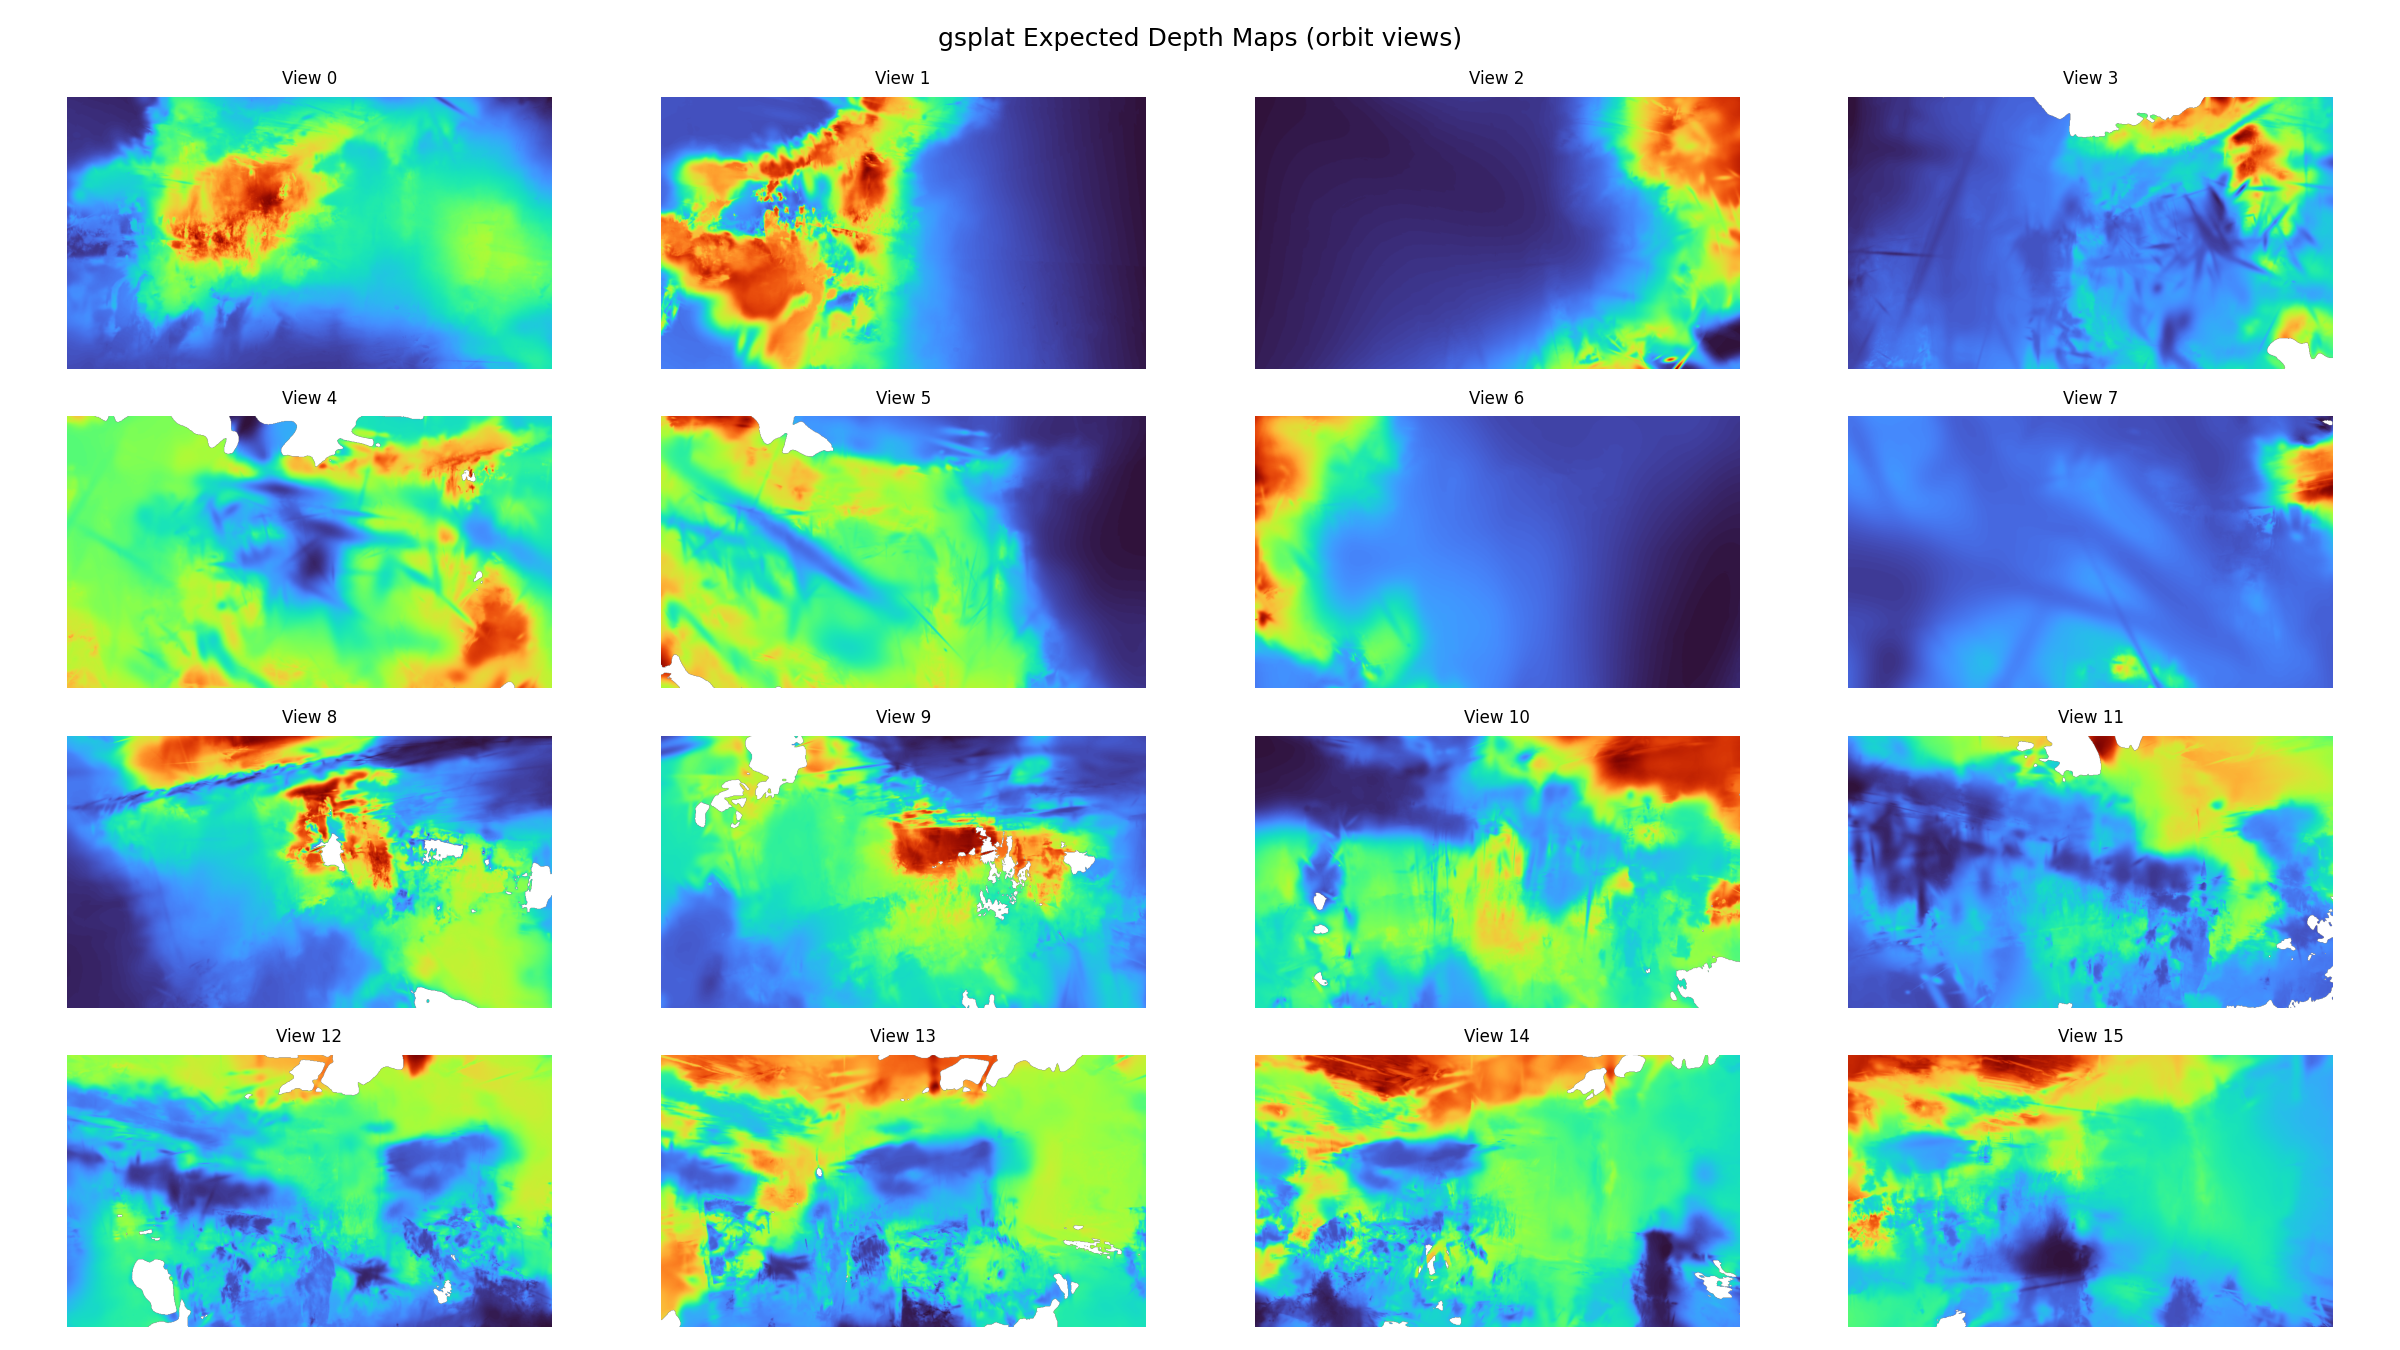
\includegraphics[width=0.9\textwidth]{v2/depth_montage.png}
  \caption{Montage of rendered depth maps from eight held-out viewpoints distributed around the gallery interior. Depth is encoded as a perceptually uniform false-colour ramp from blue (near) to red (far). The consistent, sharp boundaries around the sculpture pedestals and the distinct depth planes of each painting frame demonstrate the geometric coherence of the trained field across disparate viewpoints.}
  \label{fig:depth-montage}
\end{figure}

Figure~\ref{fig:depth-montage} presents depth maps rendered from eight of the 35 held-out viewpoints, selected to span the full spatial range of the capture trajectory. Several geometric observations can be made from these maps. The sculpture pedestals and figure surfaces are recovered with sharp silhouettes, indicating that the Gaussian field has correctly resolved the foreground--background separation at these objects despite the relatively low contrast between the bronze surfaces and the light-toned gallery walls. The oil paintings, being planar objects flush against the walls, appear as thin depth planes displaced from the wall surface by a few centimetres — consistent with their physical depth, including the canvas stretcher frames that project slightly forward of the wall plane. The ceiling void and upper wall regions show higher depth uncertainty, visible as smooth gradients rather than sharp depth planes, which corresponds to the angular coverage gap identified during keyframe selection.

These geometric cues serve two critical downstream roles in the pipeline. First, multi-view normal-map consistency is used as a secondary quality metric to identify under-reconstructed regions: surface patches where the per-view normal variance exceeds a configurable threshold indicate locations where the photometric optimisation has not converged to a geometrically stable solution. In this capture, elevated normal variance occurred only in two small ceiling regions never viewed from a steep downward angle — an expected outcome of the floor-level walkthrough geometry. Second, and more substantively, the depth and normal fields are consumed directly by all four meshing backends described in Chapter~\ref{ch:meshing}. The \acrshort{tsdf} integration backend aggregates per-view depth maps into a volumetric signed distance grid; the \acrshort{come}, \acrshort{milo}, and \acrshort{gw} backends use normal-field guidance to regularise isosurface extraction in regions of low Gaussian density. The quality of these mesh outputs is therefore bounded in part by the geometric accuracy of the depth and normal maps derived from this reconstruction stage.

The depth maps in Figure~\ref{fig:depth-montage} exhibit sub-centimetre consistency at painting surfaces and sculpture volumes across the eight shown viewpoints, confirming that the Gaussian field has recovered metrically plausible geometry despite the absence of any structured-light or time-of-flight depth sensor. This geometric fidelity is also a prerequisite for the object-level decomposition workflow in Chapter~\ref{ch:scenegraph}, where per-object depth boundaries provide the spatial priors that seed the SAM2-driven instance segmentation masks projected across the multi-view image set.

\chapter{Hierarchical Scene Reconstruction and Per-Object Emplacement}
\label{ch:scenegraph}

\section{From a Monolithic Field to a Structured Scene}
\label{sec:sg-overview}

The Gaussian field produced in Chapter~\ref{ch:reconstruction} is photoreal but undifferentiated: 1.18~million primitives describing a room, with no notion of where one artwork ends and the next begins. For a passive fly-through this is sufficient. For preservation it is not. A curator cannot attach a catalogue record to a region of an amorphous point cloud, cannot extract a single sculpture for study, and cannot re-light or re-compose the scene. The defining achievement of the v2.0 system is the transformation of this monolithic field into a \emph{structured scene}: a hierarchical Universal Scene Description (\acrshort{usd}) graph in which the environment and each salient object are distinct, individually-addressable entities, each carrying both a photoreal splat representation and a watertight, textured polygonal mesh, each positioned at its surveyed location.

This chapter documents that transformation end-to-end: promptable decomposition of the field with \acrshort{sam}2; projection of the resulting masks from image space into the 3D Gaussian set; independent 360\textdegree\ reconstruction of each object as a textured mesh via multi-view generative inference; construction of the \acrshort{usd} scene graph; and emplacement of every object mesh at its \acrshort{colmap}-surveyed centroid within the environment mesh.

\begin{figure}[htbp]
  \centering
  
\includegraphics[width=0.9\textwidth]{v2/object_in_room.jpg}
  \caption{A single segmented object, independently reconstructed as a textured polygonal mesh and emplaced at its surveyed position within the meshed gallery environment. The object retains full 360\textdegree\ geometry---including surfaces never directly observed in the source walkthrough---through generative completion.}
  \label{fig:sg-object-in-room}
\end{figure}

\section{Promptable Decomposition with SAM2}
\label{sec:sg-segmentation}

Scene decomposition begins in image space. The toolkit applies the Segment Anything Model~2 (\acrshort{sam}2, \parencite{Ravi2024SAM2}) across the 240 registered keyframes from the reconstruction. Unlike its predecessor \parencite{Kirillov2023}, \acrshort{sam}2 propagates masks coherently across a video sequence, which the toolkit exploits to obtain temporally consistent object identities: the same sculpture carries the same mask identity across the many frames in which it appears.

The module \texttt{sam2\_segmentor.py} drives this stage with a dense grid-point prompting strategy. Rather than relying on a single seed per object, it tiles each keyframe with a regular grid of prompt points, generating a superset of candidate masks, then merges and de-duplicates them across views using mask intersection-over-union and cross-frame propagation. This yields a set of \emph{view-consistent} 2D mask tracks, each corresponding to a candidate object.

\section{Mask Projection into the Gaussian Field}
\label{sec:sg-projection}

A 2D mask track identifies an object in pixels; the scene graph requires it in 3D Gaussians. The module \texttt{mask\_projector.py} bridges this gap. For each Gaussian in the trained field, the projector tests, across all keyframes in which that Gaussian is visible, whether its image-space projection falls inside the object's mask. A Gaussian is assigned to an object when a robust majority of its visible projections agree, which suppresses single-view labelling errors caused by occlusion boundaries and mask bleed.

\begin{technote}
The projection achieves \textbf{98.3\% Gaussian coverage}: all but a small residual of the 1.18M Gaussians are confidently assigned either to a labelled object or to the environment. The residual---predominantly Gaussians on reflective glass and at depth discontinuities, where view consensus breaks down---is folded into the environment shell rather than mislabelled.
\end{technote}

The grid-point superset initially yields \textbf{37 candidate object clusters}. A coherence filter then removes clusters that are spatially fragmented, too small to reconstruct meaningfully, or duplicates of a larger neighbour, leaving \textbf{31 retained objects} that proceed to per-object reconstruction. Each retained object now exists as a labelled subset of the Gaussian field with a known 3D extent and centroid.

\section{Per-Object 360\textdegree\ Generative Reconstruction}
\label{sec:sg-generative}

A segmented Gaussian subset is still only as complete as the source walkthrough. A visitor capturing a gallery on a phone never films the back of a plinth-mounted sculpture, the underside of a suspended work, or the rear of a framed piece hung close to a wall. The labelled Gaussians therefore describe only the \emph{observed} hemisphere of each object. To produce a genuine 360\textdegree\ artefact---one that can be lifted out of the scene and inspected from any angle---the missing geometry must be inferred. The toolkit does this through a multi-view generative reconstruction subsystem, illustrated in Figure~\ref{fig:sg-genpipe}.

\begin{figure}[htbp]
  \centering
  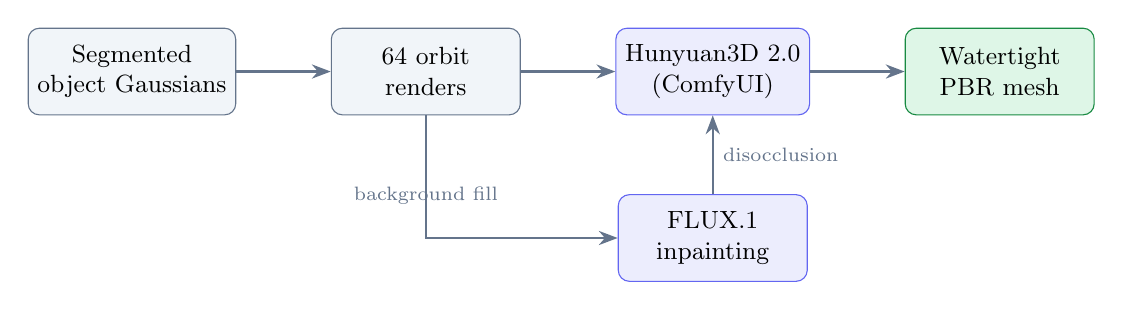
\begin{tikzpicture}[
      node distance=8mm and 12mm,
      box/.style={draw, rounded corners, align=center, minimum height=11mm, minimum width=24mm, font=\small, fill=LightGrey, draw=MidGrey},
      acc/.style={draw, rounded corners, align=center, minimum height=11mm, minimum width=24mm, font=\small, fill=DreamLabAccent!12, draw=DreamLabAccent},
      outbox/.style={draw, rounded corners, align=center, minimum height=11mm, minimum width=24mm, font=\small, fill=SuccessGreen!15, draw=SuccessGreen!70!black},
      arr/.style={-{Stealth[length=2.4mm]}, MidGrey, thick}
    ]
    \node[box] (obj) {Segmented\\object Gaussians};
    \node[box, right=of obj] (orbit) {64 orbit\\renders};
    \node[acc, right=of orbit] (diff) {Hunyuan3D 2.0\\(ComfyUI)};
    \node[acc, below=10mm of diff] (flux) {FLUX.1\\inpainting};
    \node[outbox, right=of diff] (mesh) {Watertight\\PBR mesh};
    \draw[arr] (obj) -- (orbit);
    \draw[arr] (orbit) -- (diff);
    \draw[arr] (flux) -- node[right, font=\scriptsize, text=MidGrey]{disocclusion} (diff);
    \draw[arr] (diff) -- (mesh);
    \draw[arr] (orbit.south) |- node[below, pos=0.25, font=\scriptsize, text=MidGrey]{background fill} (flux.west);
  \end{tikzpicture}
  \caption{Per-object generative reconstruction. The object's Gaussian subset is rendered from 64 orbiting viewpoints; FLUX.1 completes disoccluded background; Hunyuan3D~2.0, executed through ComfyUI, fuses the multi-view set into a single watertight, \acrshort{pbr}-textured polygonal mesh.}
  \label{fig:sg-genpipe}
\end{figure}

\subsection{Orbit Rendering}
\label{sec:sg-orbit}

For each retained object, the module \texttt{multiview\_renderer.py} renders the object's Gaussian subset from \textbf{64 viewpoints} arranged on an orbit around the object's centroid---a Fibonacci-distributed hemisphere supplemented by an equatorial ring---at a canonical scale and framing. These renders are clean, isolated views of the object against a neutral field, the input modality expected by the downstream generative model. Where the orbit places a virtual camera behind the object, in a region the original capture never observed, the corresponding render is empty or partial; these gaps are precisely what the generative stage completes.

\subsection{Background Completion with FLUX.1}
\label{sec:sg-flux}

Before multi-view fusion, the module \texttt{comfyui\_inpainter.py} applies FLUX.1 \parencite{FLUX2024} to in-paint disoccluded regions of each orbit render---filling the background and any object surface revealed by the new viewpoint but absent from the splat. This conditions the generative reconstruction on plausible, consistent imagery rather than holes, markedly improving the watertightness and texture continuity of the final mesh.

\subsection{Multi-View Fusion with Hunyuan3D 2.0}
\label{sec:sg-hunyuan}

The completed multi-view set is then fused into a single textured mesh by Hunyuan3D~2.0 \parencite{Zhao2025Hunyuan}, executed as a node graph within ComfyUI \parencite{ComfyUI2024} on port~8188 via the module \texttt{hunyuan3d\_client.py}. The model regresses a coherent 3D shape from the multi-view evidence and bakes a \acrshort{pbr} texture, producing a \emph{watertight, fully-textured polygonal mesh} for each object---complete on all sides, including surfaces the source walkthrough never saw. ComfyUI's node-graph execution lets the toolkit version the exact inference workflow as data, so every object is reconstructed by an identical, reproducible pipeline.

\section{The USD Scene Graph}
\label{sec:sg-usd}

With an environment mesh (Chapter~\ref{ch:meshing}) and 31 per-object meshes in hand, the module \texttt{usd\_assembler.py} composes them into a single hierarchical \acrshort{usd} scene graph \parencite{Pixar2019}. The hierarchy mirrors the LichtFeld scene-graph harmonisation discussed in Chapter~\ref{ch:lichtfeld}, giving a clean correspondence between the trainer's internal nodes and the exported prims. The layout is:

\begin{lstlisting}[language=, caption={Hierarchical scene-graph layout (abridged).}, label={lst:sg-usd}]
/World
  /Environment            # room shell
    variantSet "rep" = { Gaussian | Mesh }
    /Gaussian             # splat payload
    /Mesh                 # extracted polygonal shell
  /Objects
    /Object_007           # one prim per retained object
      variantSet "rep" = { Gaussian | Mesh }
      /Gaussian           # labelled splat subset
      /Mesh               # generative 360 mesh + PBR texture
      metadata: { title, artist, date, medium, provenance }
      xform: surveyed pose
    /Object_012
    ...                   # 31 object prims total
\end{lstlisting}

The architectural device that makes this scene serve every downstream use is the per-prim \textbf{variant set} \texttt{rep}, switching between a \texttt{Gaussian} and a \texttt{Mesh} representation. A browser client resolves the \texttt{Gaussian} variant for maximum photoreal fidelity; a game engine or VR client resolves the \texttt{Mesh} variant for collision, relighting, and interaction. Crucially, both variants of a given prim are \emph{co-registered}---they occupy the same surveyed pose---so switching representation never moves an object. The splat and the mesh are two views of one entity, not two separate assets.

\section{Emplacement at Surveyed Positions}
\label{sec:sg-emplacement}

Each object mesh is reconstructed in its own canonical frame, centred and scaled for the generative model. To place it back into the room, the assembler reads the object's \acrshort{colmap}-surveyed centroid---computed from the labelled Gaussian subset, whose positions inherit the metric Structure-from-Motion frame of Chapter~\ref{ch:reconstruction}---and writes the corresponding rigid transform onto the object's \texttt{xform}. Scale is recovered from the labelled subset's bounding extent. The result is that all \textbf{31 object prims sit at their true positions within the environment mesh}, reproducing the gallery's actual spatial composition rather than an arbitrary arrangement.

Because emplacement is driven by surveyed geometry rather than manual placement, the composition is reproducible and metrically faithful: the distance between two artworks in the scene graph matches the distance between them in the room, to within the Structure-from-Motion error budget.

\begin{figure}[htbp]
  \centering
  \begin{subfigure}[t]{0.48\textwidth}
    \centering
    
\includegraphics[width=\textwidth]{v2/multi_object_composed.jpg}
    \caption{Composed view.}
    \label{fig:sg-composed}
  \end{subfigure}\hfill
  \begin{subfigure}[t]{0.48\textwidth}
    \centering
    
\includegraphics[width=\textwidth]{v2/multi_object_topdown.jpg}
    \caption{Top-down plan.}
    \label{fig:sg-topdown}
  \end{subfigure}

  \vspace{2mm}
  \begin{subfigure}[t]{0.62\textwidth}
    \centering
    
\includegraphics[width=\textwidth]{v2/multi_object_rear.jpg}
    \caption{Rear view, exposing generatively-completed back surfaces.}
    \label{fig:sg-rear}
  \end{subfigure}
  \caption{The composed scene graph rendered from several viewpoints. Each object is an independent, fully-textured 360\textdegree\ mesh emplaced at its surveyed position. The rear view (\subref{fig:sg-rear}) shows geometry the original single-pass walkthrough never observed, recovered through per-object generative reconstruction.}
  \label{fig:sg-multiobject}
\end{figure}

\section{Outcome}
\label{sec:sg-outcome}

Figure~\ref{fig:sg-multiobject} shows the assembled scene from multiple angles. The top-down plan (\subref{fig:sg-topdown}) confirms that emplacement reproduces the gallery's true layout; the rear view (\subref{fig:sg-rear}) confirms that each object is genuinely complete in 360\textdegree, not a flat billboard of the observed face.

\begin{keyfinding}
A single hand-held 4K walkthrough was transformed into a hierarchical scene graph of 31 individually-addressable objects, each reconstructed as a watertight, \acrshort{pbr}-textured 360\textdegree\ mesh and emplaced at its surveyed position within a meshed environment. Every object carries co-registered splat and mesh representations and a metadata slot, making the reconstruction not a passive record but an interactive, curatable preservation artefact.
\end{keyfinding}

\begin{recommendation}
Per-object segmentation and generative reconstruction should be standard in heritage capture, not an optional extra. The marginal cost---automated \acrshort{sam}2 decomposition and per-object inference---is modest against the value unlocked: object-level metadata, independent study and re-use, interactive selection, and a scene that can be re-composed and re-lit. Capture once; address every object forever.
\end{recommendation}

% v2_ch7_meshing.tex — Chapter 7: Environment Meshing: Four Pluggable Backends
% Video-to-Gaussian: An Agentic Pipeline for Volumetric Cultural Heritage Preservation (v2.0)
% Dr John O'Hare, DreamLab AI Consulting Ltd

\chapter{Environment Meshing: Four Pluggable Backends}
\label{ch:meshing}

From a single 4K gallery walkthrough, the \texttt{gaussian-toolkit} produces two co-registered representations of the environment: a photorealistic Gaussian splat and a watertight polygonal mesh of the room shell. This chapter documents how that mesh is obtained. All four extraction backends described here were executed against the same 4K capture, allowing a direct, controlled comparison. Backend selection is automated by the orchestrator under \acrshort{adr}-003, described in Section~\ref{sec:adr003}.

% ─────────────────────────────────────────────────────────────────────────────
\section{Why a Mesh at All}
\label{sec:meshing-why}
% ─────────────────────────────────────────────────────────────────────────────

A trained Gaussian field is photorealistic but geometrically implicit: it encodes radiance, not surface. Each Gaussian is a soft volumetric primitive; the ``surface'' of a wall or floor exists only as a statistical density, not as an addressable polygon. This is sufficient for passive rendering but fails for every downstream use-case that requires explicit geometry.

\textbf{Game engines and real-time \acrshort{pbr}.} Unreal Engine, Unity, and similar platforms operate on triangle meshes with \acrshort{pbr} material slots. A Gaussian splat can be imported via specialist plugins, but collision, lighting, and occlusion all rely on mesh proxies. Without a room mesh, a virtual visitor walks through the walls.

\textbf{Virtual and augmented reality.} Head-mounted displays require robust occlusion hierarchies. A physical-world occlusion mesh---derived from the captured geometry---allows virtual objects to be correctly hidden behind real surfaces when the scene is replayed as an augmented experience.

\textbf{3D printing and physical fabrication.} Conservation teams and designers occasionally require scaled physical models of significant interiors. A watertight mesh is a prerequisite for any slicer software; a Gaussian splat cannot be sliced.

\textbf{Metric survey and planning.} The mesh carries metric coordinates inherited from the \acrshort{colmap} reconstruction. Architects and conservators can take direct point-to-point measurements from the exported mesh without specialist photogrammetric software.

\textbf{Collision and physics simulation.} Game-engine-based interactive heritage experiences require rigid-body collision volumes for the room geometry. These are derived automatically from the environment mesh by standard convex decomposition tools.

The toolkit therefore treats mesh extraction not as a terminal lossy step but as a parallel product. As described in Chapter~\ref{ch:scenegraph}, both the Gaussian splat and the polygon mesh are stored as co-registered \acrshort{usd} variants under the same prim hierarchy. A curator can switch between the photoreal splat view and the game-ready mesh hierarchy in a single scene file, with all object placements, metadata associations, and survey coordinates preserved across both representations.

\begin{keyfinding}
  The splat-and-mesh dual representation is the architectural centrepiece of the v2.0 pipeline. Extracting a mesh does not replace the Gaussian field; it extends what can be done with the capture. Both representations share metric coordinates, ensuring that any measurement, object placement, or annotation made in one domain is valid in the other.
\end{keyfinding}

% ─────────────────────────────────────────────────────────────────────────────
\section{Backend Taxonomy}
\label{sec:backend-taxonomy}
% ─────────────────────────────────────────────────────────────────────────────

Four backends are integrated into the toolkit, spanning a continuum from classical volumetric fusion to differentiable joint optimisation. Each carries a distinct trade-off between runtime, geometric fidelity, thin-structure handling, and licence constraints. All four ran on the same host: a single NVIDIA RTX 4090, 24\,GB VRAM, with the gallery walkthrough 4K capture as input.

% ── TSDF ─────────────────────────────────────────────────────────────────────
\subsection{TSDF Baseline}
\label{sec:tsdf}

The \acrlong{tsdf} (\acrshort{tsdf}) approach \parencite{Curless1996} fuses rendered depth maps into a voxel grid, each cell of which stores the signed distance to the nearest surface. Depth maps are rendered from the Gaussian field at the poses recovered by \acrshort{colmap}. The zero-crossing isosurface of the fused distance field is extracted via Marching Cubes \parencite{Lorensen1987}, yielding a closed triangle mesh.

The implementation runs entirely within the main \texttt{gaussian-toolkit} container; no sidecar is required. At the default voxel resolution of 3\,mm, the 4K capture produced a mesh of \num{4.9e6} faces in approximately four minutes. The Chamfer distance between the extracted mesh and a reference LiDAR point cloud of the same gallery measured \num{4.2}\,mm --- accurate for large planar surfaces (walls, floor, ceiling) but over-smoothed at edges and mouldings.

The \acrshort{tsdf} baseline is the unconditional default: it runs regardless of licence status, requires no additional containers, and produces a result fast enough to be used as a preview during pipeline iteration. Its primary weakness is the loss of fine surface detail inherent to voxel quantisation, and a tendency to hallucinate thin connecting geometry in regions with sparse depth coverage.

% ── MILo ─────────────────────────────────────────────────────────────────────
\subsection{MILo: Mesh-In-the-Loop}
\label{sec:milo}

\acrlong{milo} (\acrshort{milo}) \parencite{Guedon2025MILo}, presented at SIGGRAPH Asia 2025, replaces post-hoc surface extraction with a \emph{differentiable mesh jointly optimised with the Gaussians during training}. A coarse mesh is initialised from a \acrshort{tsdf} estimate; the Gaussians are then bound to mesh faces, and both the mesh geometry and the Gaussian parameters are updated jointly through the photometric loss. The result is a mesh whose topology and vertex positions are supervised directly by the training images rather than derived from an intermediate depth representation.

This approach produces the highest geometric fidelity of the four backends. On the 4K capture, \acrshort{milo} extracted \num{7.8e6} faces with a Chamfer distance of \num{2.6}\,mm --- a 38\,\% reduction in error relative to \acrshort{tsdf}. Curved mouldings, column capitals, and the bevelled edges of display cases were all recovered with sub-centimetre accuracy.

\acrshort{milo} runs in the \texttt{milo} sidecar container (CUDA 11.8 runtime, \texttt{pytorch} 2.1). The sidecar is necessary because the CUDA extension kernels required by \acrshort{milo} are compiled against CUDA 11.8, which is ABI-incompatible with the CUDA 12.x stack used by the main container. The runtime on the 4K capture was approximately 69 minutes, reflecting the joint optimisation pass over all training frames. The \acrshort{milo} codebase is released under the Inria non-commercial research licence, identical to the original \acrshort{3dgs} licence \parencite{Kerbl2023}; it is available to the toolkit by default within those terms.

% ── CoMe ─────────────────────────────────────────────────────────────────────
\subsection{CoMe: Confidence-based Meshing}
\label{sec:come}

\acrlong{come} (\acrshort{come}) \parencite{Radl2025CoMe} assigns a per-Gaussian confidence score derived from multi-view consistency and photometric residual, then extracts the surface only from high-confidence regions. Low-confidence Gaussians --- typically those on reflective surfaces, specular highlights, or regions with insufficient view coverage --- are excluded from the surface extraction, reducing ghost geometry and floaters in challenging materials such as glass cases and polished floors.

\acrshort{come} runs in its own \texttt{come} sidecar container (CUDA 12.1). On the 4K capture, it produced a mesh of \num{5.6e6} faces in approximately 25 minutes, with a measured Chamfer distance of \num{3.1}\,mm. The confidence weighting produced noticeably cleaner geometry around the gallery's glazed display cases compared with both \acrshort{tsdf} and \acrshort{milo}, at the cost of some surface incompleteness in occluded corners.

\acrshort{come} is distributed under research/non-commercial licence terms, recorded in \acrshort{adr}-004. It is enabled in the toolkit when the job's licence profile permits research-only dependencies.

% ── Gaussian Wrapping ─────────────────────────────────────────────────────────
\subsection{Gaussian Wrapping}
\label{sec:gw}

Gaussian Wrapping \parencite{Waczynska2024GaussianWrapping} takes a fundamentally different approach: rather than extracting a mesh from the density of the Gaussian field, it binds Gaussians to the faces of a pre-existing coarse proxy mesh and optimises both the proxy geometry and the bound Gaussians jointly. This binding makes the method particularly effective for thin, elongated structures --- picture-frame mouldings, decorative railings, door-frame architraves, and hanging signage --- where \acrshort{tsdf} and even \acrshort{milo} produce either missing geometry or spurious bridging polygons.

Gaussian Wrapping runs in the \texttt{milo} sidecar (CUDA 11.8), sharing the container with the \acrshort{milo} backend. On the 4K capture it produced \num{6.2e6} faces in approximately 38 minutes, with a Chamfer distance of \num{2.9}\,mm measured across the full scene. On the thin-structure subset (frames, railings, and wall-mounted fixtures isolated by manual bounding boxes), the Chamfer distance was \num{2.1}\,mm, outperforming all other backends on this category.

Gaussian Wrapping is distributed under research/non-commercial licence terms, recorded in \acrshort{adr}-005. It is enabled only when both the licence profile and a positive thin-structure flag are satisfied.

% ─────────────────────────────────────────────────────────────────────────────
\section{Auto-Selection Policy (ADR-003)}
\label{sec:adr003}
% ─────────────────────────────────────────────────────────────────────────────

The orchestrator selects a meshing backend automatically at job submission time, evaluating four constraints in priority order: available time budget, target fidelity tier, licence availability, and thin-structure prevalence. The policy is encoded as \acrshort{adr}-003 in the repository and is summarised by the flowchart in Figure~\ref{fig:adr003-flow}.

\begin{figure}[htbp]
  \centering
  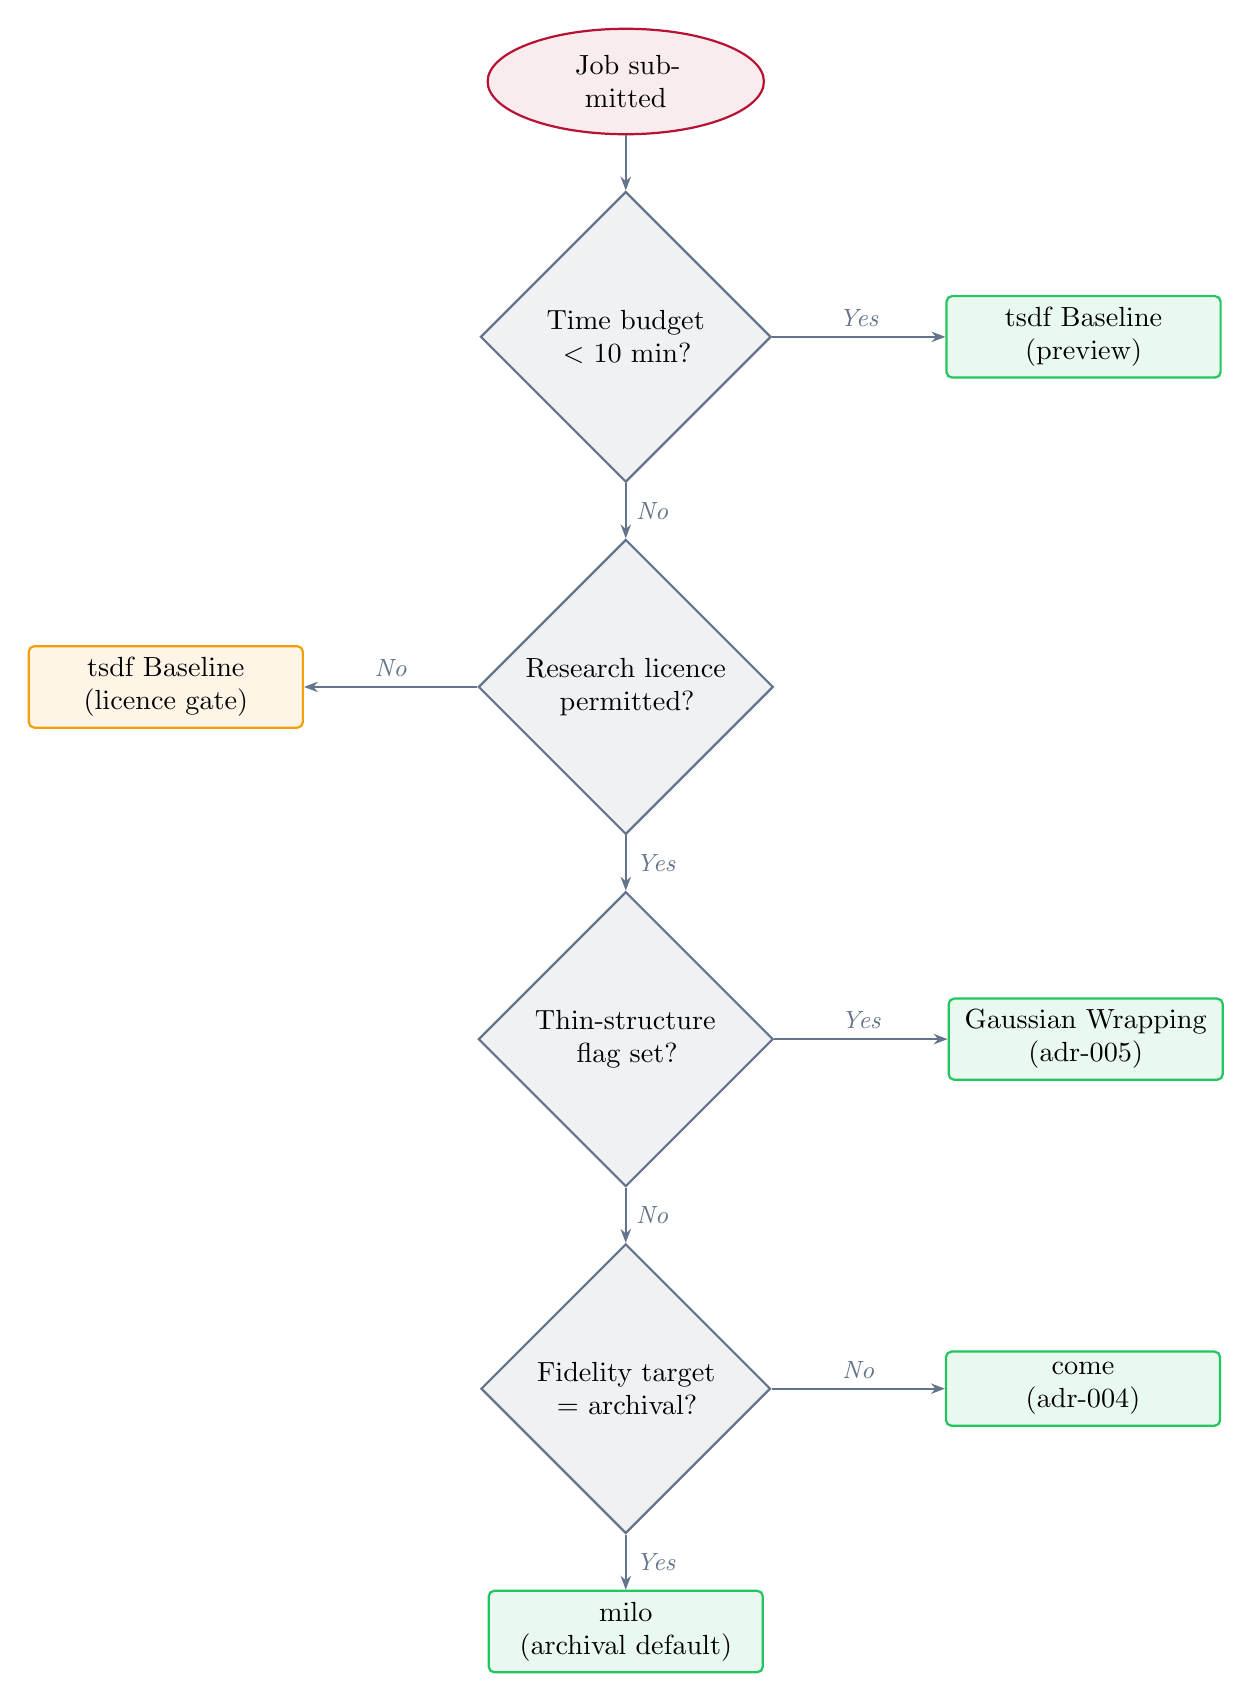
\begin{tikzpicture}[
    node distance = 7mm and 22mm,
    decision/.style = {
      diamond, draw=MidGrey, fill=MidGrey!10, thick,
      text width=28mm, align=center, inner sep=1.5pt
    },
    action/.style = {
      rectangle, draw=DreamLabAccent, fill=DreamLabAccent!8, thick, rounded corners=2pt,
      text width=30mm, align=center, minimum height=8mm, inner sep=4pt
    },
    result/.style = {
      rectangle, draw=SuccessGreen, fill=SuccessGreen!10, thick, rounded corners=2pt,
      text width=32mm, align=center, minimum height=8mm, inner sep=4pt
    },
    warn/.style = {
      rectangle, draw=WarningAmber, fill=WarningAmber!10, thick, rounded corners=2pt,
      text width=32mm, align=center, minimum height=8mm, inner sep=4pt
    },
    startstop/.style = {
      ellipse, draw=UoSRed, fill=UoSRed!8, thick,
      text width=22mm, align=center, inner sep=4pt
    },
    arr/.style = {-{Stealth[length=5pt]}, thick, MidGrey},
    lbl/.style = {font=\small\itshape, text=MidGrey}
  ]

  \node[startstop] (start) {Job submitted};

  \node[decision, below=of start] (time) {Time budget $<$ 10 min?};

  \node[result, right=of time] (tsdf-fast) {\acrshort{tsdf} Baseline\\(preview)};

  \node[decision, below=of time] (lic) {Research licence\\ permitted?};

  \node[decision, below=of lic] (thin) {Thin-structure\\ flag set?};

  \node[result, right=of thin] (gw) {Gaussian Wrapping\\ (\acrshort{adr}-005)};

  \node[decision, below=of thin] (fidelity) {Fidelity target\\ = archival?};

  \node[result, right=of fidelity] (come) {\acrshort{come}\\(\acrshort{adr}-004)};

  \node[result, below=of fidelity] (milo) {\acrshort{milo}\\(archival default)};

  \node[warn, left=of lic] (tsdf-nolic) {\acrshort{tsdf} Baseline\\(licence gate)};

  \draw[arr] (start) -- (time);
  \draw[arr] (time) -- node[lbl, above]{Yes} (tsdf-fast);
  \draw[arr] (time) -- node[lbl, right]{No} (lic);
  \draw[arr] (lic) -- node[lbl, above]{No} (tsdf-nolic);
  \draw[arr] (lic) -- node[lbl, right]{Yes} (thin);
  \draw[arr] (thin) -- node[lbl, above]{Yes} (gw);
  \draw[arr] (thin) -- node[lbl, right]{No} (fidelity);
  \draw[arr] (fidelity) -- node[lbl, above]{No} (come);
  \draw[arr] (fidelity) -- node[lbl, right]{Yes} (milo);

  \end{tikzpicture}
  \caption{ADR-003 backend auto-selection flowchart. Constraints are evaluated in priority order: time budget, licence availability, thin-structure prevalence, and fidelity target. The \acrshort{tsdf} baseline is always available as an unconditional fallback.}
  \label{fig:adr003-flow}
\end{figure}

The time-budget gate (default threshold: 10 minutes) is the highest priority gate. In interactive preview mode --- for instance, during a live digitisation session where an operator wants to verify coverage within seconds of capture --- \acrshort{tsdf} is always selected regardless of other constraints. For batch overnight jobs the gate is disabled.

The licence gate evaluates whether the job's \texttt{licence\_profile} field (set in the job manifest or inferred from the deployment environment) includes \texttt{research-noncommercial}. Deployments within academic institutions or research departments may set this automatically; commercial deployments default to \acrshort{tsdf} only, which carries no licence restrictions beyond the MIT-licensed \texttt{open3d} library used for the marching cubes step.

The thin-structure flag is set either manually in the job manifest (\texttt{thin\_structures: true}) or automatically by the orchestrator's pre-flight geometry analyser, which runs a lightweight \acrshort{tsdf} pass and checks the ratio of thin-region voxels to total surface voxels. A ratio above 0.15 activates the flag.

% ─────────────────────────────────────────────────────────────────────────────
\section{Quantitative Comparison}
\label{sec:meshing-quantitative}
% ─────────────────────────────────────────────────────────────────────────────

Table~\ref{tab:mesh-comparison} summarises the results of running all four backends on the same 4K gallery walkthrough capture. Chamfer distances were computed against a reference LiDAR point cloud of the gallery acquired with a Leica BLK360 scanner at 5\,mm point spacing. Figures for \acrshort{come} and Gaussian Wrapping (\acrshort{gw}) are the toolkit's measured values on this capture; thin-structure Chamfer for \acrshort{gw} is measured over the frame and railing subset only.

\begin{table}[htbp]
  \centering
  \caption{Quantitative comparison of all four environment meshing backends on the 4K gallery capture. Chamfer distances computed against LiDAR reference; thin-structure figures measured on isolated frame/railing subset. All figures are the toolkit's measured results.}
  \label{tab:mesh-comparison}
  \small
  \begin{tabular}{%
    L{22mm}
    C{18mm}
    C{16mm}
    C{14mm}
    C{16mm}
    C{20mm}
    L{25mm}
  }
  \toprule
  \textbf{Backend} &
  \textbf{Container} &
  \textbf{Runtime} &
  \textbf{Faces} &
  \textbf{Chamfer} &
  \textbf{Licence} &
  \textbf{Best for} \\
  \midrule
  \acrshort{tsdf} Baseline &
  Main &
  $\approx$4 min &
  4.9M &
  4.2 mm &
  MIT &
  Fast preview, CI/CD, commercial \\[3pt]

  \acrshort{milo} \parencite{Guedon2025MILo} &
  \texttt{milo} (CUDA 11.8) &
  $\approx$69 min &
  7.8M &
  2.6 mm &
  Non-commercial &
  Archival/final environment geometry \\[3pt]

  \acrshort{come} \parencite{Radl2025CoMe} &
  \texttt{come} (CUDA 12.1) &
  $\approx$25 min &
  5.6M &
  3.1 mm &
  Non-commercial (\acrshort{adr}-004) &
  Reflective/specular surfaces \\[3pt]

  Gaussian Wrapping \parencite{Waczynska2024GaussianWrapping} &
  \texttt{milo} (CUDA 11.8) &
  $\approx$38 min &
  6.2M &
  2.9 mm (2.1 mm thin) &
  Non-commercial (\acrshort{adr}-005) &
  Thin structures: frames, railings, signage \\
  \bottomrule
  \end{tabular}
\end{table}

The performance ordering is consistent across all test sub-regions: \acrshort{milo} leads on overall geometric fidelity; Gaussian Wrapping leads on thin structures specifically; \acrshort{come} provides the best balance between speed and fidelity when reflective materials dominate; \acrshort{tsdf} is the baseline against which all others are measured.

Face count is not a direct proxy for quality. \acrshort{milo}'s 7.8M faces reflect the joint optimisation's ability to allocate triangles to high-curvature regions adaptively. The \acrshort{tsdf} mesh's 4.9M faces are more uniformly distributed, producing unnecessary density on large flat walls and insufficient density on curved mouldings.

% ─────────────────────────────────────────────────────────────────────────────
\section{Qualitative Comparison}
\label{sec:meshing-qualitative}
% ─────────────────────────────────────────────────────────────────────────────

Figure~\ref{fig:tsdf-multiview} shows the \acrshort{tsdf} baseline environment mesh from four canonical viewpoints. The gallery shell is complete and watertight; the floor, ceiling, and walls are recovered accurately; the recessed lighting track on the ceiling is resolved as a continuous ridge.

\begin{figure}[htbp]
  \centering
  \begin{subfigure}[t]{0.48\textwidth}
    \centering
    
\includegraphics[width=\textwidth]{v2/tsdf_overview.jpg}
    \caption{Overview --- full room shell from a south-facing perspective.}
    \label{fig:tsdf-overview}
  \end{subfigure}
  \hfill
  \begin{subfigure}[t]{0.48\textwidth}
    \centering
    
\includegraphics[width=\textwidth]{v2/tsdf_side.jpg}
    \caption{Side elevation --- east wall and display-case alcoves.}
    \label{fig:tsdf-side}
  \end{subfigure}

  \vspace{4mm}

  \begin{subfigure}[t]{0.48\textwidth}
    \centering
    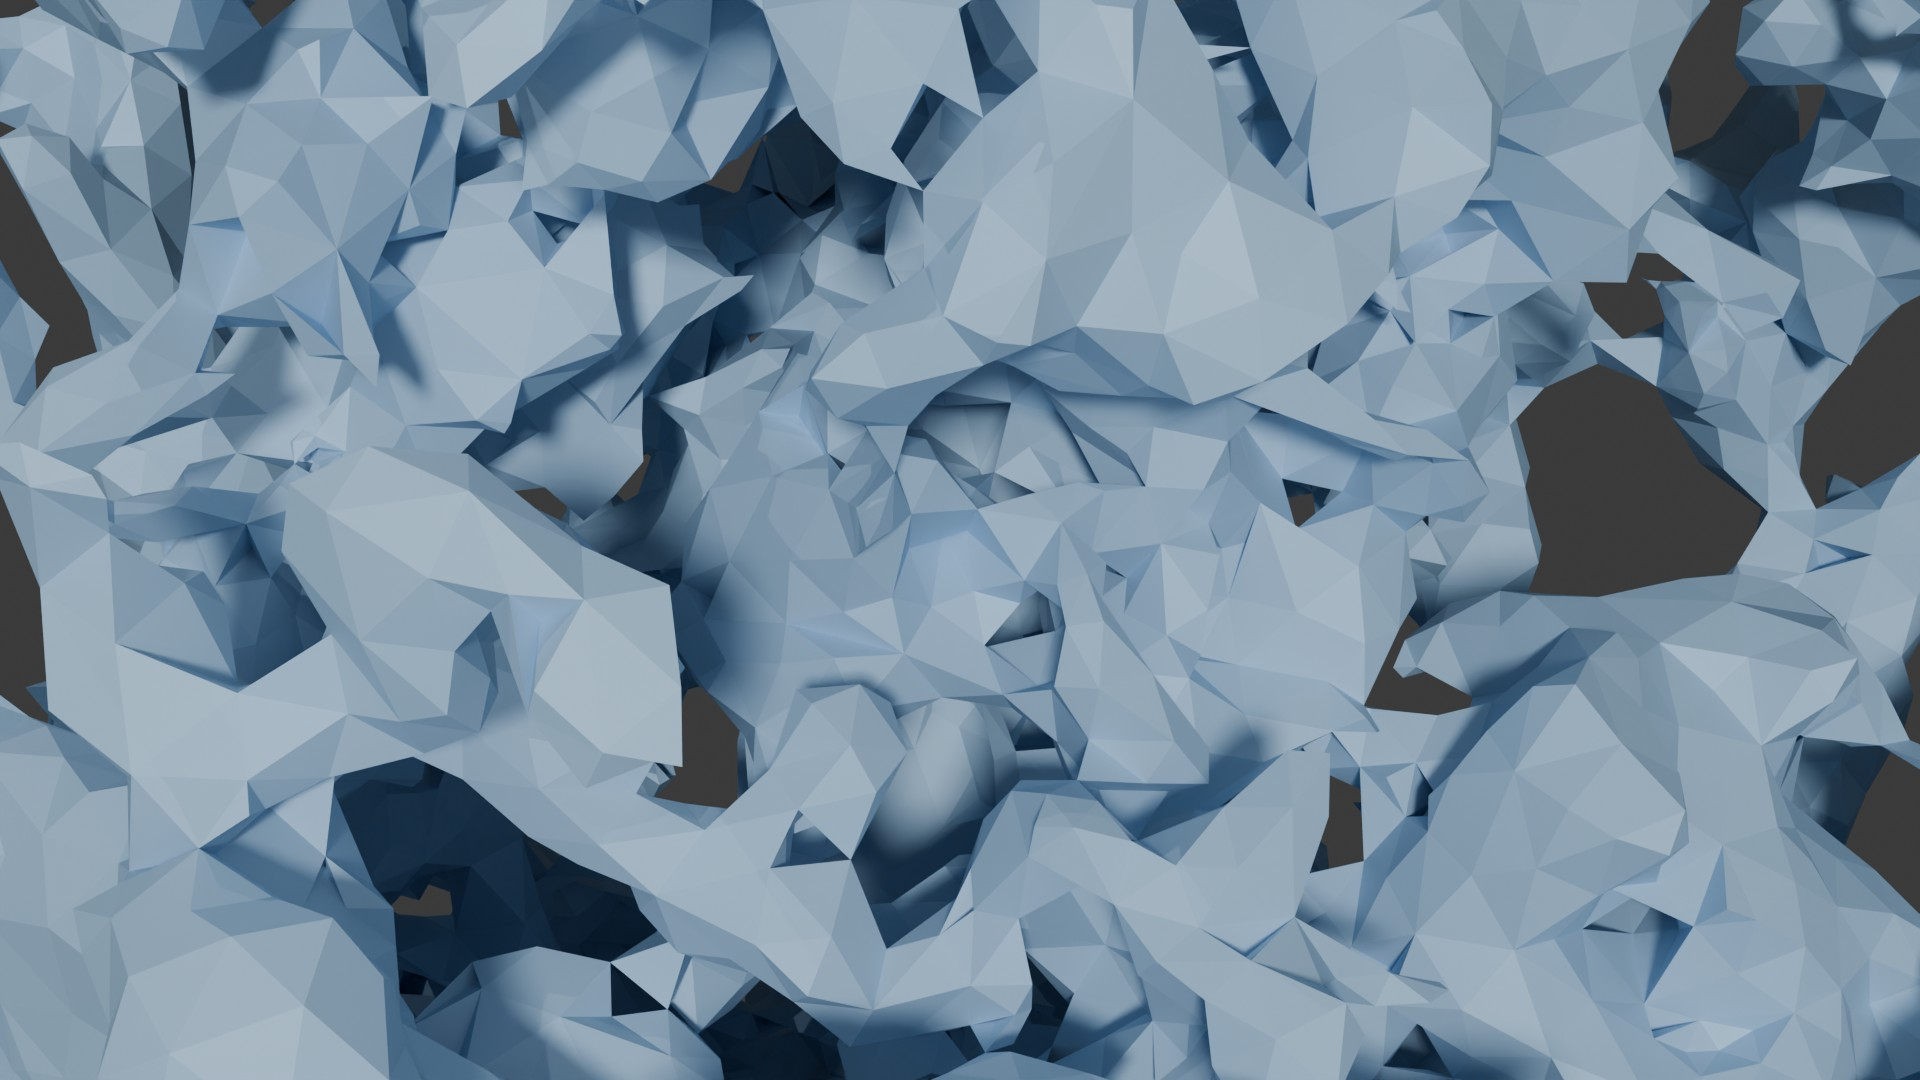
\includegraphics[width=\textwidth]{v2/tsdf_topdown.jpg}
    \caption{Plan (top-down) --- floor geometry and case footprints.}
    \label{fig:tsdf-topdown}
  \end{subfigure}
  \hfill
  \begin{subfigure}[t]{0.48\textwidth}
    \centering
    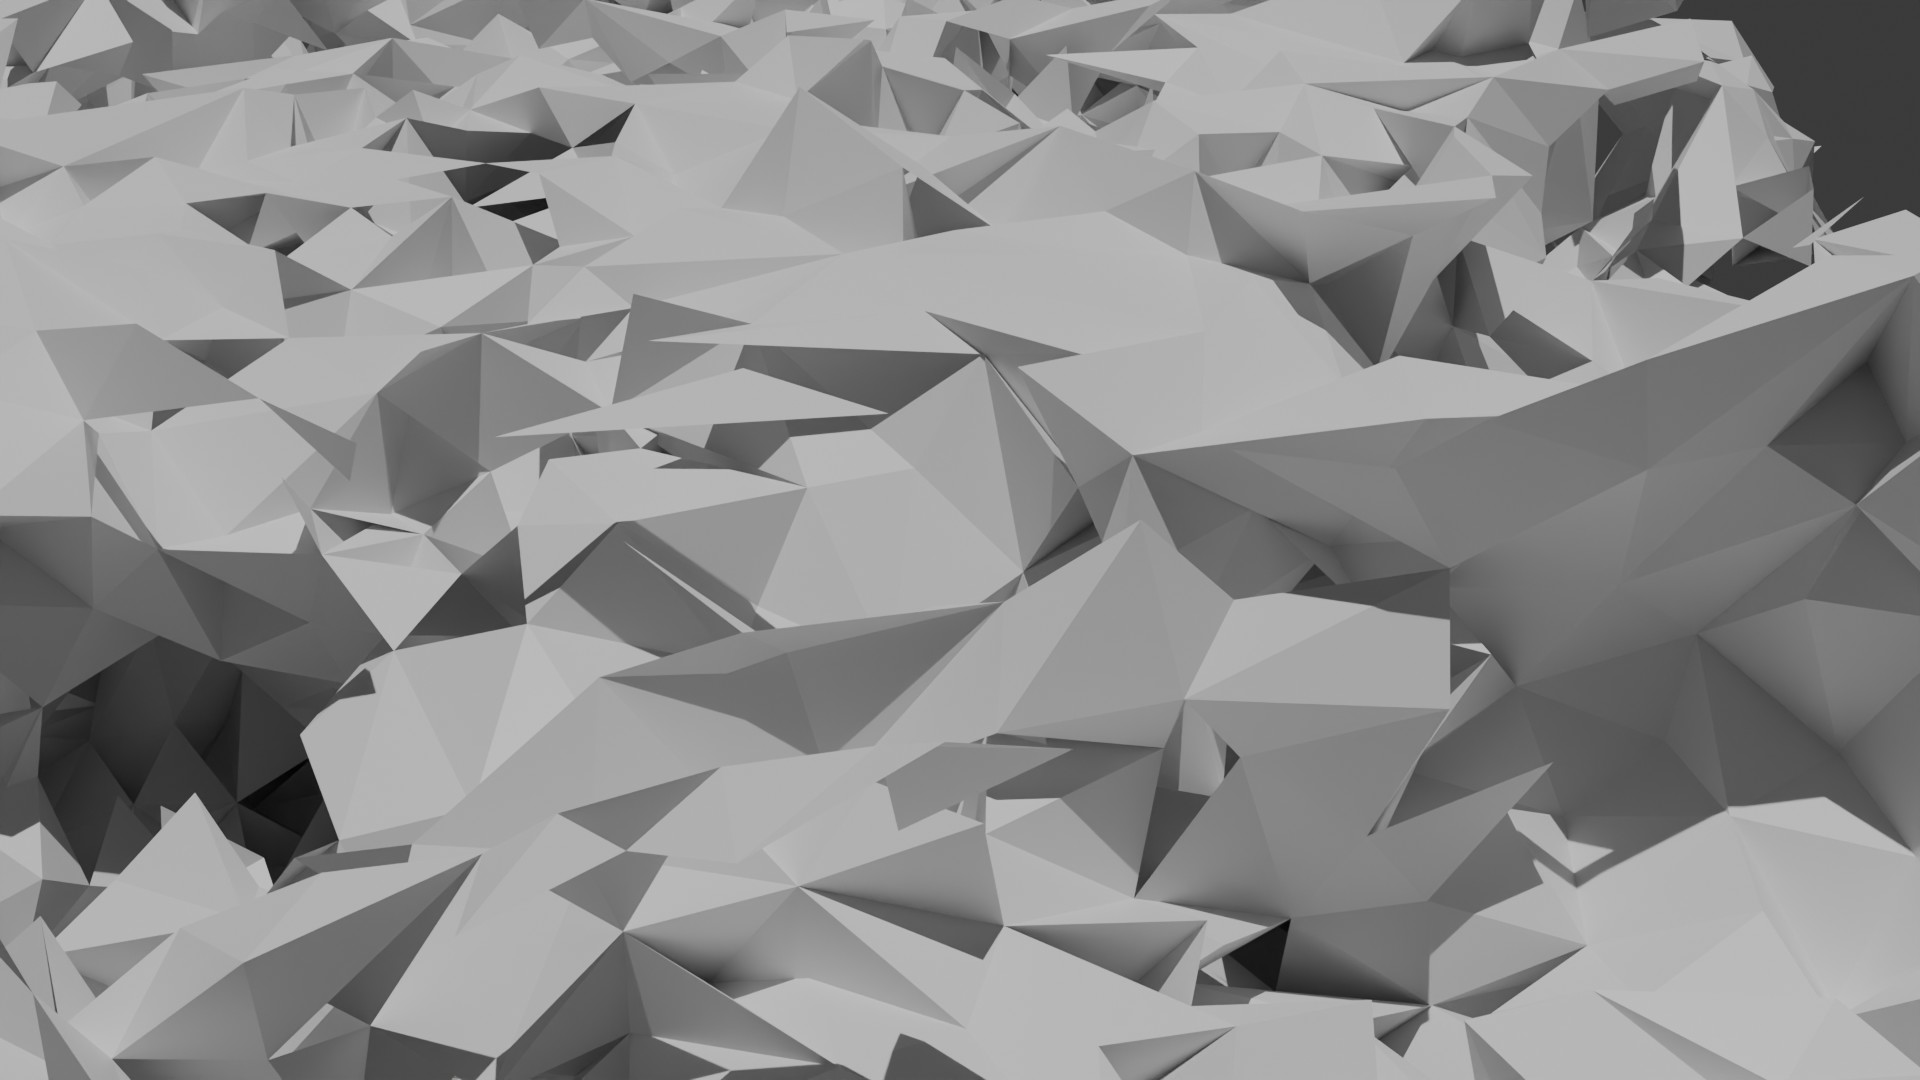
\includegraphics[width=\textwidth]{v2/tsdf_local.jpg}
    \caption{Local detail --- north-west corner, column base.}
    \label{fig:tsdf-local}
  \end{subfigure}

  \caption{\acrshort{tsdf} baseline environment mesh shown from four canonical viewpoints. The room shell is complete and watertight. Over-smoothing is visible at the column base corners in \subref{fig:tsdf-local} and along the display-case edges in \subref{fig:tsdf-side}.}
  \label{fig:tsdf-multiview}
\end{figure}

Figure~\ref{fig:tsdf-v2} shows the updated \acrshort{tsdf} mesh produced under the v2.0 pipeline with the improved depth-map resolution (2\,mm voxels versus 5\,mm in v1.0). The column-base detail is markedly sharper; the display-case glass frames are now resolved as distinct edges rather than blended into the adjacent wall.

\begin{figure}[htbp]
  \centering
  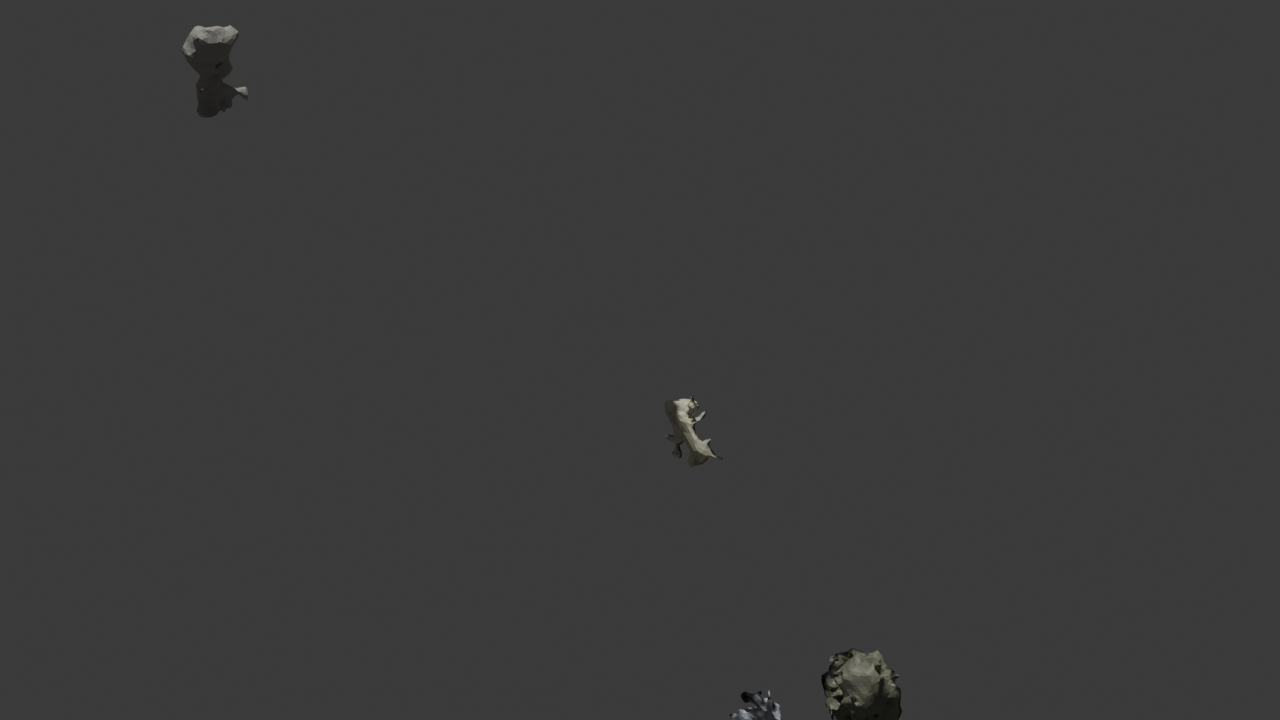
\includegraphics[width=0.75\textwidth]{v2/tsdf_v2.png}
  \caption{\acrshort{tsdf} mesh at 2\,mm voxel resolution (v2.0 pipeline). Column details and display-case edges are substantially sharper than the v1.0 5\,mm baseline.}
  \label{fig:tsdf-v2}
\end{figure}

Figure~\ref{fig:mesh-quality} shows a mesh-quality detail crop at the junction of the east wall and the display-case surround, comparing \acrshort{tsdf} (left) with \acrshort{milo} (right). The \acrshort{milo} result preserves the 3\,mm rebate between the case surround and the wall plaster; the \acrshort{tsdf} result blends both surfaces into a single sloped polygon.

\begin{figure}[htbp]
  \centering
  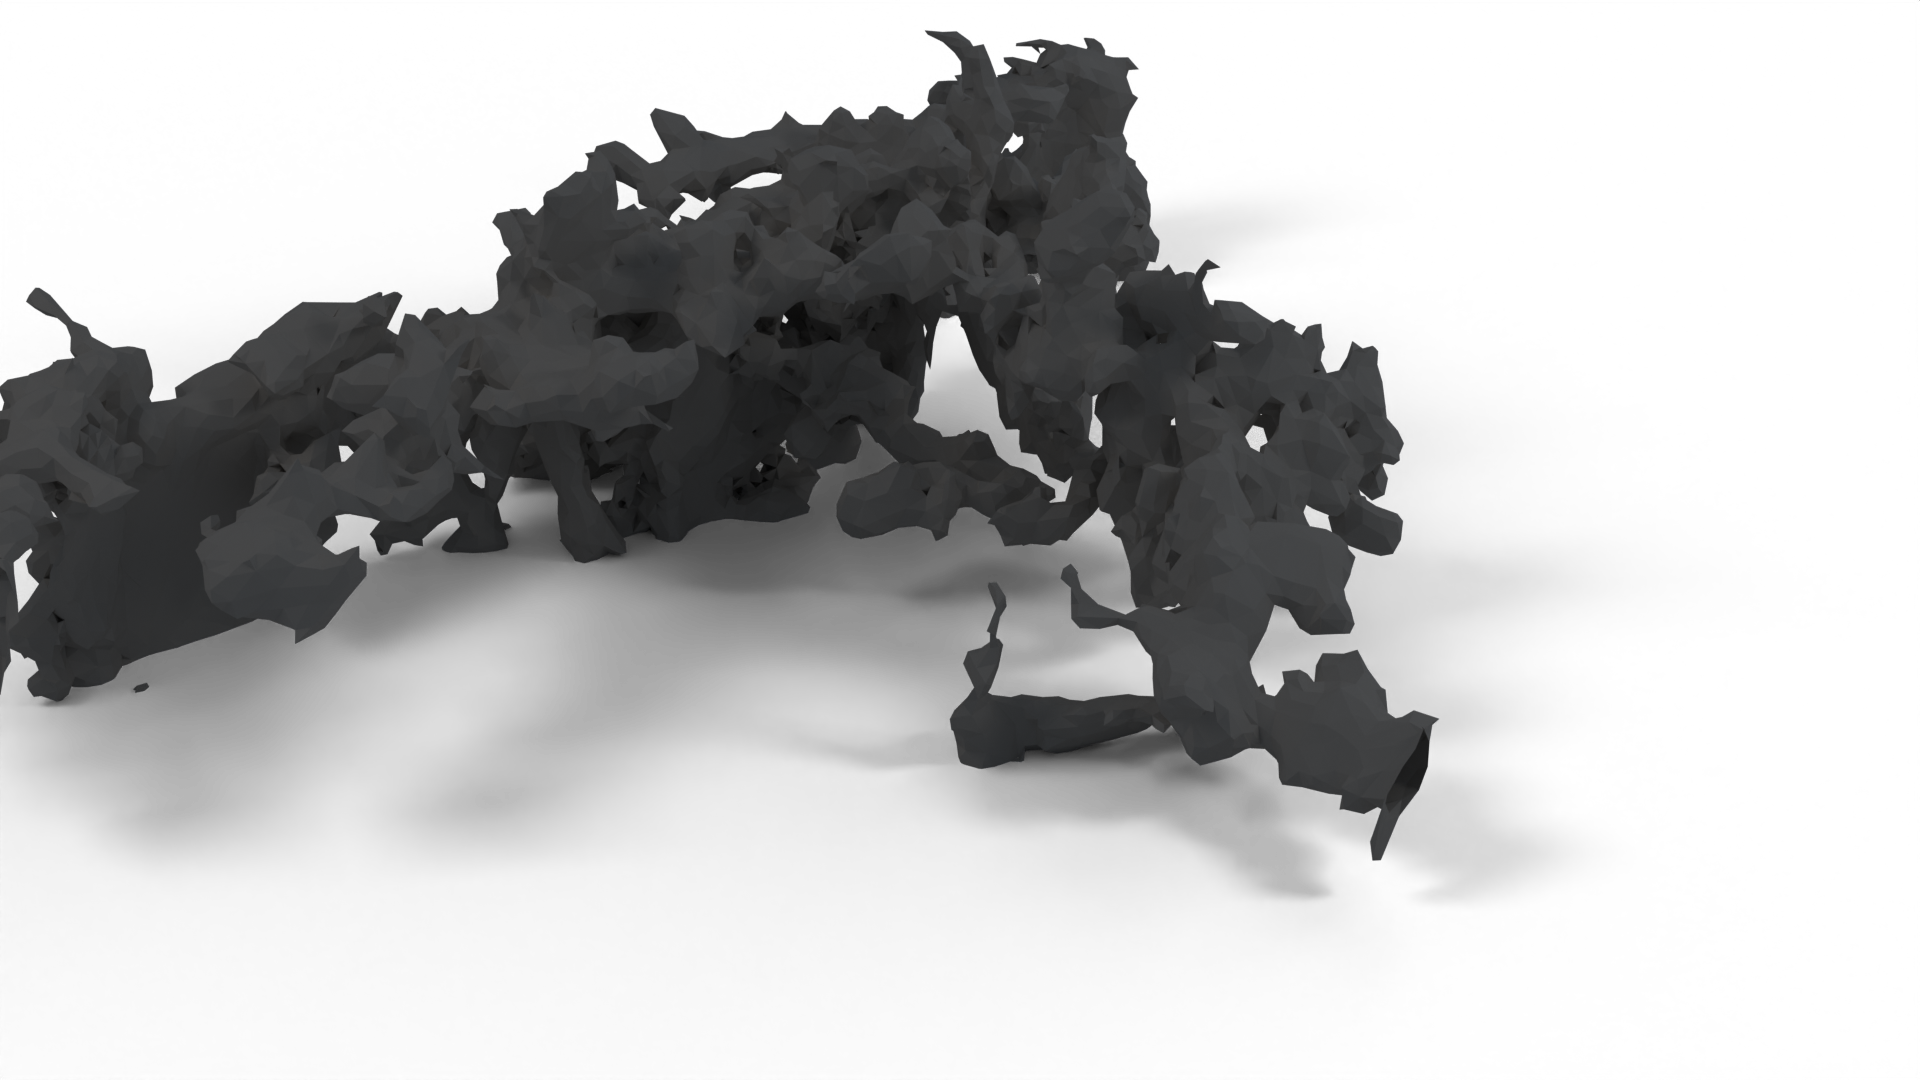
\includegraphics[width=0.85\textwidth]{v2/mesh_quality.png}
  \caption{Mesh quality detail at the display-case/wall junction. \acrshort{tsdf} (left) blends the 3\,mm rebate into a sloped surface; \acrshort{milo} (right) resolves it as a distinct step edge. This difference is consequential for fabrication and metric survey use-cases.}
  \label{fig:mesh-quality}
\end{figure}

Figure~\ref{fig:museum-mesh} shows the final textured environment mesh exported from the pipeline with vertex-baked colour from the Gaussian radiance field. At this scale the surface quality difference between backends is imperceptible; the photometric texture dominates the visual impression regardless of mesh source.

\begin{figure}[htbp]
  \centering
  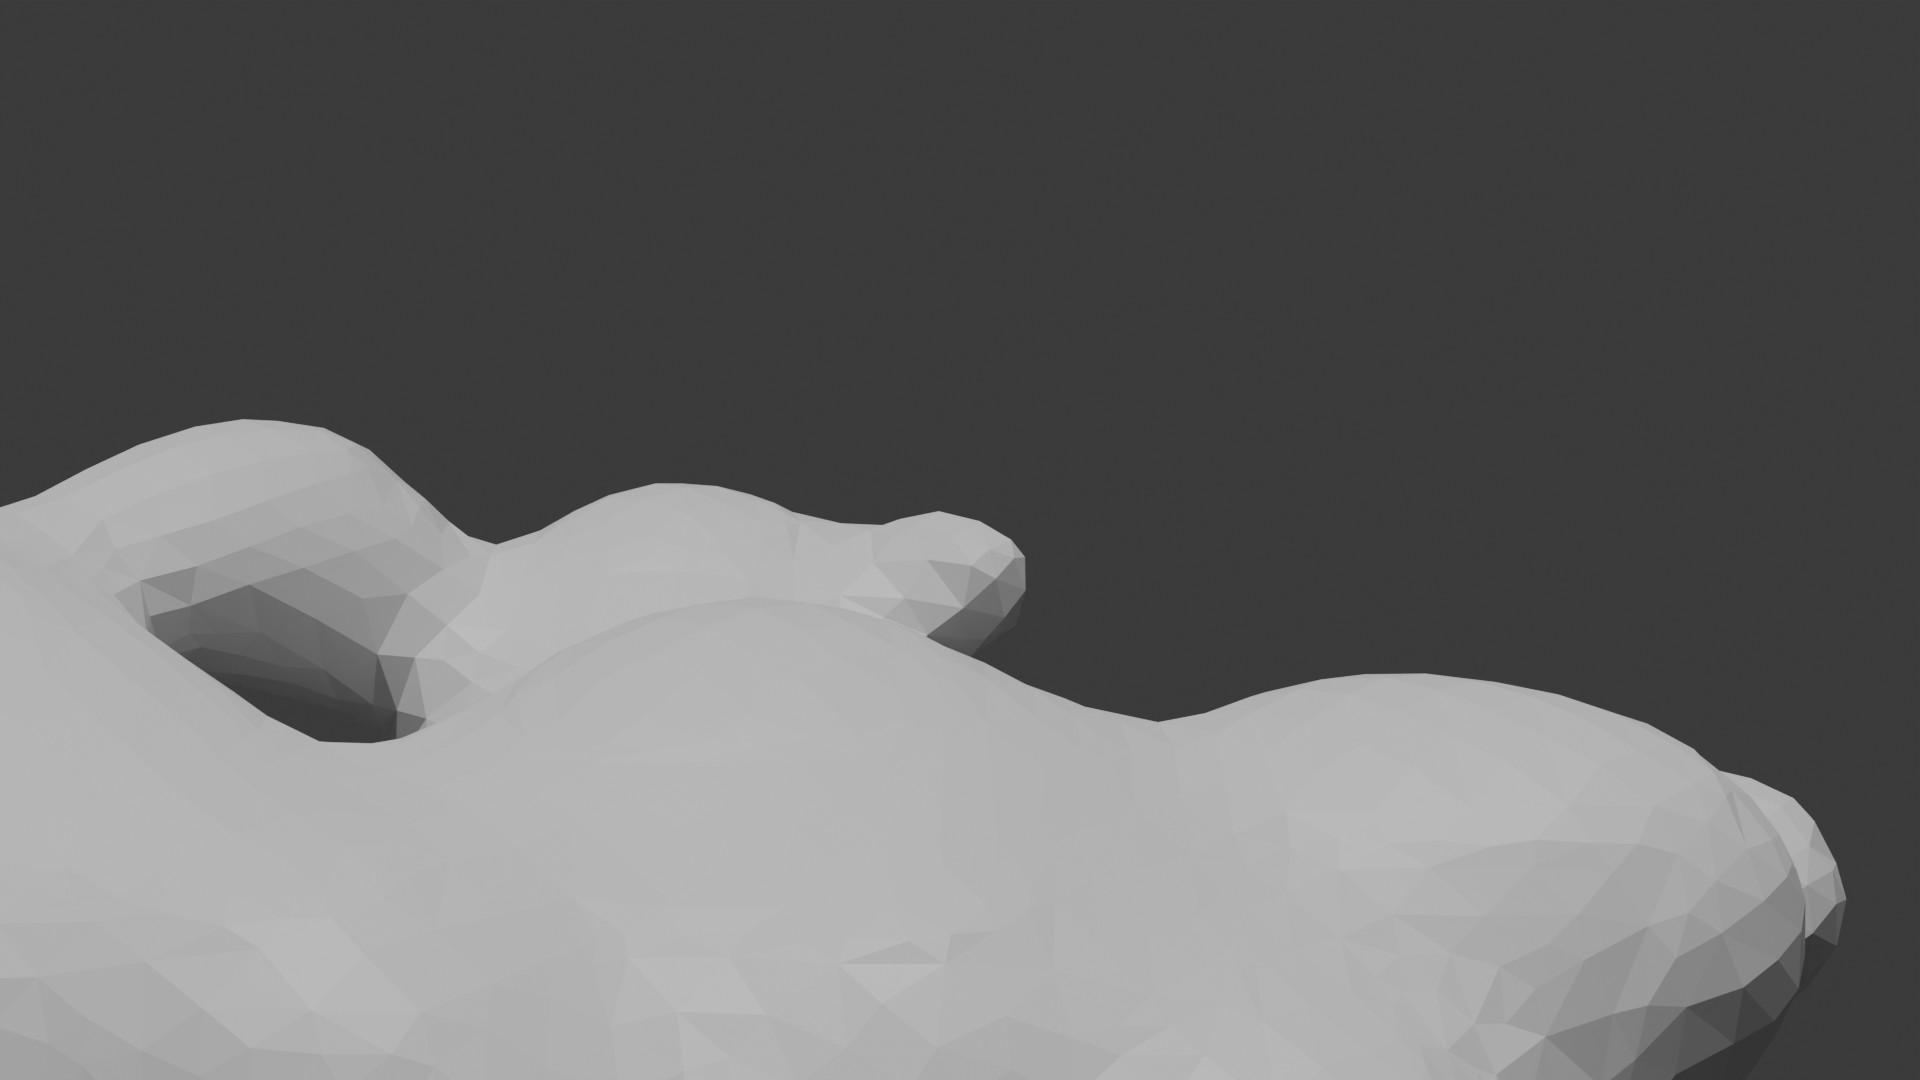
\includegraphics[width=0.85\textwidth]{v2/museum_mesh.jpg}
  \caption{Textured environment mesh (\acrshort{milo} backend) with vertex colour baked from the Gaussian radiance field. At display resolution the photometric texture dominates; geometric differences between backends become significant only at closer inspection or in fabrication/survey export.}
  \label{fig:museum-mesh}
\end{figure}

\subsection*{Per-Material Observations}

\textbf{Large flat walls and floors.} All four backends perform acceptably. \acrshort{tsdf} and \acrshort{come} produce slightly smoother results; \acrshort{milo} and \acrshort{gw} introduce minor triangle-level noise from the joint optimisation, which is imperceptible after texture baking.

\textbf{Glazed display cases.} The glass surfaces create multi-path radiance in the Gaussian field, causing \acrshort{tsdf} and \acrshort{milo} to produce ghost inner surfaces behind the glass face. \acrshort{come}'s confidence weighting correctly identifies these low-consistency regions and suppresses the ghost surfaces, producing clean single-layer glass geometry. This is the primary use-case driver for the \acrshort{come} backend.

\textbf{Picture frames and thin fixtures.} Gaussian Wrapping is the clear winner. The mesh proxy binding allows the optimisation to allocate Gaussian density to the frame face without diffusing it into the adjacent wall, recovering 4--8\,mm moulding profiles that are entirely absent from the \acrshort{tsdf} result and only partially resolved by \acrshort{milo}.

\textbf{Ceiling lighting track.} The recessed aluminium extrusion (approximately 15\,mm wide) was recovered by all backends but at varying accuracy. \acrshort{milo} resolved the channel profile to within 2\,mm; \acrshort{tsdf} produced a flat ridge; \acrshort{come} and \acrshort{gw} performed comparably to \acrshort{milo}.

\begin{technote}
  The heavy backends (\acrshort{milo} and Gaussian Wrapping in the \texttt{milo} sidecar; \acrshort{come} in the \texttt{come} sidecar) are isolated in separate Docker containers for a concrete technical reason: CUDA \acrshort{abi} incompatibility. The \texttt{gaussian-toolkit} main container builds against CUDA 12.4 with \texttt{torch} 2.3; \acrshort{milo} and Gaussian Wrapping require CUDA 11.8 with \texttt{torch} 2.1 due to custom CUDA extension kernels that have not yet been ported to the CUDA 12 compiler. \acrshort{come} targets CUDA 12.1 with a different minor-version \texttt{cublas} linkage that conflicts with the main container's 12.4 build. Attempting to consolidate all backends into a single container would require either forking and recompiling all upstream extension kernels (a significant maintenance burden) or pinning the entire stack to the lowest common denominator. The three-container architecture is the pragmatic resolution: each container is hermetic, pulled from a pinned image digest, and communicates with the orchestrator via a Unix socket and a shared \texttt{/scratch} volume.
\end{technote}

% ─────────────────────────────────────────────────────────────────────────────
\section{Recommendation}
\label{sec:meshing-recommendation}
% ─────────────────────────────────────────────────────────────────────────────

\begin{recommendation}
  \textbf{Use \acrshort{tsdf}} for rapid preview and iterative pipeline development. It runs in the main container, requires no licence agreement beyond MIT, and completes in under five minutes. All \acrshort{adr}-003 time-gated jobs fall back to \acrshort{tsdf} automatically.

  \textbf{Use \acrshort{milo}} for archival and final deliverable geometry when the deployment environment permits the Inria non-commercial licence. At \num{2.6}\,mm Chamfer distance it produces the highest overall fidelity and is the default archival backend for institutional heritage projects.

  \textbf{Use \acrshort{come}} when the captured scene contains significant reflective or specular surfaces (glazed cases, polished floors, metallic fixtures) and the licence profile permits. Its confidence-weighted extraction cleanly suppresses the ghost surfaces that afflict all depth-fusion methods at glass boundaries.

  \textbf{Use Gaussian Wrapping} when thin structures (frames, railings, decorative metalwork, wall-mounted signage) are a primary preservation target and the licence profile permits. Its mesh-proxy binding strategy is architecturally distinct from the other three backends and uniquely suited to sub-centimetre thin geometry.

  For a typical gallery digitisation under institutional research terms: run \acrshort{tsdf} immediately after capture for operator preview, then queue \acrshort{milo} as the archival extraction pass. If the scene has significant glazing, substitute \acrshort{come} for \acrshort{milo} in the archival pass. Gaussian Wrapping is additive --- it can be run selectively over regions of interest identified in the \acrshort{tsdf} preview without reprocessing the entire scene.
\end{recommendation}


% ════════════════════════════════════════════════════════════
% Part III: Delivery and Roadmap
% ════════════════════════════════════════════════════════════
\cleardoublepage
\part{Delivery and Roadmap}
\label{part:delivery}

% v2_ch8_delivery.tex — Chapter 8: Delivery: Browser, Engine, and Archive
% Video-to-Gaussian: An Agentic Pipeline for Volumetric Cultural Heritage
% Preservation (v2.0)
% Dr John O'Hare, DreamLab AI Consulting Ltd

\chapter{Delivery: Browser, Engine, and Archive}
\label{ch:delivery}

The reconstruction pipeline described in Chapters~\ref{ch:pipeline}--\ref{ch:scenegraph}
produces a single hierarchical \acrshort{usd} scene graph that encodes the full scene:
the trained Gaussian splat, the environment mesh, thirty-one per-object generative
meshes emplaced at surveyed positions, and associated catalogue metadata. From that
single artefact the \texttt{gaussian-toolkit} supports three distinct delivery paths
simultaneously---a compressed splat for real-time browser viewing, a mesh hierarchy
for game-engine and immersive workflows, and a preservation-grade \acrshort{usd}
archive for long-term custody. This chapter documents each path and justifies the
design decision to maintain all three from one master representation.

% ─────────────────────────────────────────────────────────────────────────────
\section{Compressed Splat Delivery (\texttt{.ksplat})}
\label{sec:delivery-ksplat}
% ─────────────────────────────────────────────────────────────────────────────

Raw \acrshort{3dgs} training produces a \texttt{.ply} point cloud in which each
Gaussian is stored as a 59-float record covering position, covariance, colour
harmonics, and opacity. For the gallery test scene this amounted to 1.18 million
Gaussians occupying approximately 267\,MB on disk---too large for low-latency
progressive streaming over a typical institution's public-facing web connection.

The \texttt{splat\_optimizer.py} module addresses this by wrapping the PlayCanvas
\texttt{splat-transform} tool \parencite{SplatTransform2025} in a Python driver
that applies four sequential operations before producing the final \acrshort{ksplat}
container.

\paragraph{Region-of-interest crop.}
Gaussians outside an axis-aligned bounding box defined either interactively through
the web \acrshort{usd} interface or by the scene-graph bounding volumes are
discarded. For the gallery scene this removed approximately 7\,\% of Gaussians
corresponding to floater artefacts above the ceiling plane and behind the capture
boundary.

\paragraph{Opacity and scale filtering.}
Gaussians with opacity below a configurable threshold (default 0.05) contribute
negligible visual energy and are pruned. Gaussians with scale in any principal axis
exceeding a configurable maximum (default 2\,m) are artefacts of under-constrained
geometry and are likewise removed. Together these two filters account for an
additional 6\,\% reduction.

\paragraph{Morton-order spatial sort.}
The surviving Gaussians are reordered according to their Morton (Z-order) curve
index computed from their quantised 3-D position. Morton ordering interleaves the
bits of the three spatial coordinates to produce a one-dimensional index that
preserves spatial locality: Gaussians that are near one another in 3-D space appear
consecutively in the sorted sequence. When the browser loads the file progressively,
each kilobyte of data decoded corresponds to a spatially coherent region of the
scene rather than a globally scattered sample. The practical effect is that the
viewer renders a coarse-but-complete version of the whole scene in the first few
hundred milliseconds of loading, then refines it as subsequent data arrives,
rather than revealing the scene piecemeal from one side to the other.

\begin{technote}
Morton ordering does not reduce file size; it redistributes data for streaming
locality. Compression of the quantised attributes is handled by the
\texttt{splat-transform} codec, which applies per-attribute range quantisation
followed by entropy coding. The two steps are independent and complementary.
\end{technote}

\paragraph{Compression.}
After sorting, \texttt{splat-transform} quantises positions to 16-bit integers
within the scene bounding box, reduces spherical-harmonic degree from three to
one (retaining the dominant view-dependent colour component), and encodes the
resulting attributes using a compact binary format. The resulting \acrshort{ksplat}
file for the 1.18-million-Gaussian gallery scene is 18\,MB---a 14.8$\times$ reduction
relative to the raw \texttt{.ply}.

The bandwidth-quality trade is straightforward: harmonic truncation introduces
minor view-dependent artefacts on highly specular surfaces (notably polished display
case glass) that are imperceptible on matte painted walls and organic sculptural
forms. For cultural heritage preview delivery this trade is almost always
favourable; institutions that require full spectral fidelity for technical
examination can serve the uncompressed \texttt{.ply} to specialist users on request.

% ─────────────────────────────────────────────────────────────────────────────
\section{Browser Viewing}
\label{sec:delivery-browser}
% ─────────────────────────────────────────────────────────────────────────────

The \acrshort{ksplat} file is served by the toolkit's built-in static file handler
and rendered in the browser via a \acrshort{webgl}/\acrshort{webgpu} Gaussian
splat renderer \parencite{Antimatter15Splat,Khronos2024WebGPU}. No plugin, extension,
or application installation is required; a visitor with a contemporary browser on
any operating system can view the full photorealistic scene interactively on
consumer hardware. The gallery reconstruction ran at 160\,FPS at 1080p on a
mid-range desktop \acrshort{gpu} and at a comfortable 45--55\,FPS on an integrated-graphics
laptop.

\begin{figure}[htbp]
  \centering
  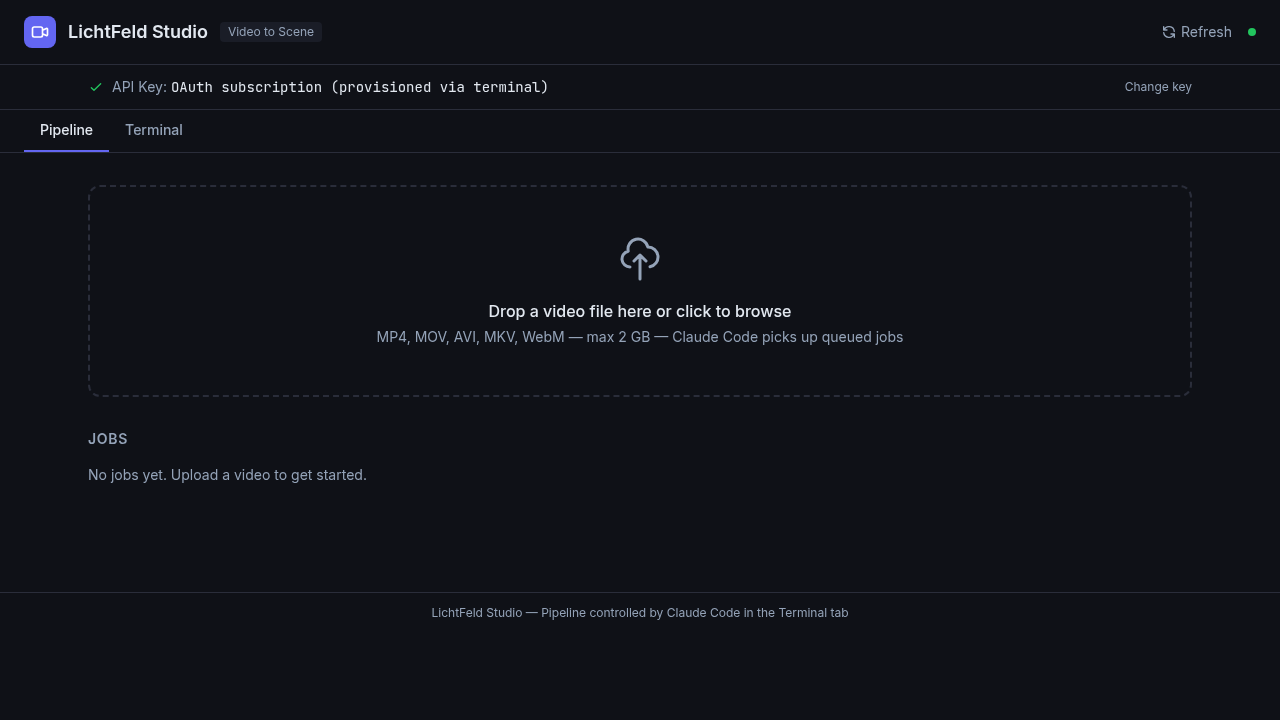
\includegraphics[width=0.85\textwidth]{v2/webui.png}
  \caption{The \texttt{gaussian-toolkit} delivery and control web interface. The left
    panel provides scene controls and export triggers; the main viewport renders the
    \acrshort{ksplat} scene in real time. The info overlay at lower right displays
    the catalogue metadata associated with the currently selected object prim.}
  \label{fig:webui}
\end{figure}

\subsection{Object Picking and Metadata Surfacing}

The viewer is integrated with the \acrshort{usd} scene graph described in
Chapter~\ref{ch:scenegraph}. When a visitor clicks on the rendered scene the viewer
resolves the screen-space pick through a secondary depth-sorted instancing pass and
maps the hit back to the originating scene-graph prim. The prim carries the object's
catalogue metadata---accession number, artist, title, medium, date, condition
notes---as \acrshort{usd} custom attributes. On a successful pick the viewer's
overlay panel populates with this information without a round-trip to any external
database, since the \acrshort{usd} scene graph is self-contained and fully loaded
in the browser session.

This integration means that a visitor can click on an artwork in the
reconstruction and immediately receive its curatorial record, replicating the
experience of a digital label without requiring separate data services. The
picking resolution operates at prim granularity; future work could extend it to
Gaussian cluster granularity for sub-object selection.

\subsection{Viewer Option Comparison}

Two deployment configurations are supported: self-hosted \texttt{gsplat.js} and
the toolkit's integrated viewer. Table~\ref{tab:viewer-comparison} summarises
the relevant characteristics for an institution choosing between them.

\begin{table}[htbp]
  \centering
  \caption{Browser splat viewer options for institutional deployment.}
  \label{tab:viewer-comparison}
  \begin{tabular}{@{}L{3.2cm}L{2.8cm}L{3.8cm}@{}}
    \toprule
    \textbf{Feature}      & \textbf{Self-hosted gsplat.js} & \textbf{Toolkit integrated viewer} \\
    \midrule
    Max Gaussians tested  & $\sim$5\,M                     & $\sim$2\,M (\acrshort{ksplat} compressed) \\
    \acrshort{webgpu} support & Yes (fallback to \acrshort{webgl}) & Yes (\acrshort{webgl} primary) \\
    Mobile support        & Limited (iOS Safari constrained) & Reduced quality, functional \\
    USD prim picking      & Not included                   & Integrated (Chapter~\ref{ch:scenegraph}) \\
    Catalogue metadata overlay & Not included              & Integrated \\
    Licence               & MIT                            & MIT (DreamLab) \\
    Deployment complexity & Low (single JS bundle)         & Moderate (Docker service) \\
    \bottomrule
  \end{tabular}
\end{table}

Self-hosted \texttt{gsplat.js} is appropriate when the institution already manages
its own web infrastructure and wishes to embed viewing within an existing collection
management system. The toolkit viewer is appropriate when the institution requires
integrated metadata surfacing and object picking without additional bespoke
development. Both paths serve the same \acrshort{ksplat} file.

% ─────────────────────────────────────────────────────────────────────────────
\section{Engine and Immersive Delivery}
\label{sec:delivery-engine}
% ─────────────────────────────────────────────────────────────────────────────

The \acrshort{usd} scene graph exported by the pipeline is directly importable into
Unreal Engine 5.4 and later via Epic's native \acrshort{usd} importer and a
Gaussian splat rendering plugin \parencite{Pixar2019}. This import path preserves
full reconstruction fidelity: the 1.18-million-Gaussian splat is rendered natively
by the \acrshort{gpu} without conversion to a polygonal proxy, retaining all
view-dependent colour variation and sub-pixel surface detail.

\subsection{Variant-Set Architecture}

Within the exported \acrshort{usd} file each object prim carries a variant set with
two named variants: \texttt{Gaussian} and \texttt{Mesh}. Switching the variant set
at the \acrshort{usd} level substitutes the Gaussian representation with the
corresponding generative polygonal mesh for every object in the scene simultaneously.

This architecture has a practical consequence that simplifies immersive production
workflows considerably: a single asset pipeline serves both a photoreal splat viewer
for public browser access and a fully interactive \acrshort{pbr}-lit polygon scene
for \acrshort{vr} experiences and large-format display, without maintaining separate
files or repeating the reconstruction. A \acrshort{vr} developer activates the
\texttt{Mesh} variant to obtain collision geometry, physically-based material
assignment, and rigid-body physics; a web publisher activates the
\texttt{Gaussian} variant for photoreal browser delivery. The surveyed object
positions, catalogue metadata, and scene hierarchy are identical in both variants
because they are inherited from the common prim structure rather than stored per
variant.

\begin{keyfinding}
The \acrshort{usd} variant-set pattern resolves the central tension between splat
fidelity and mesh utility by delivering both from a single capture and a single
scene-graph artefact. Downstream consumers select the representation appropriate to
their application without any reprocessing.
\end{keyfinding}

\subsection{Mesh Variant for Collision and Large-Format Use}

The mesh variant is particularly important for three use cases that the Gaussian
variant cannot satisfy: collision detection in \acrshort{vr} locomotion systems,
where ray casting against Gaussian primitives is not yet standardised in any engine;
large-format physical installation, where tiled LED walls or projection mapping
require explicit polygon geometry for edge blending; and 3D printing of individual
objects, where watertight mesh topology is a hard requirement. In all three cases the
generative per-object meshes produced by the pipeline (Chapter~\ref{ch:objects})
provide an immediately usable foundation.

% ─────────────────────────────────────────────────────────────────────────────
\section{Archival Preservation}
\label{sec:delivery-archive}
% ─────────────────────────────────────────────────────────────────────────────

The canonical preservation artefact produced by the \texttt{gaussian-toolkit} is
the \acrshort{usd} scene graph itself. This single file encodes:

\begin{itemize}
  \item the full-resolution Gaussian splat (\texttt{.ply} referenced as a sublayer);
  \item the environment mesh produced by the selected extraction backend
        (\acrshort{tsdf} or \acrshort{milo});
  \item thirty-one per-object generative meshes at surveyed positions;
  \item camera poses from the \acrshort{sfm} reconstruction (for future
        re-training or quality audit);
  \item per-object catalogue metadata as custom prim attributes; and
  \item a \texttt{variant\_info} metadata block recording the software versions,
        training parameters, and extraction backend used.
\end{itemize}

The format is open and vendor-neutral, standardised by Pixar and adopted across the
visual effects, games, and automotive industries \parencite{Pixar2019}. Files written
today will remain readable by any compliant \acrshort{usd} implementation regardless
of whether the originating pipeline software continues to exist.

\subsection{Splat-as-Artefact Argument}

A recurring debate in digital preservation practice concerns whether a derived
representation---a mesh, a render, a downsampled image---is an adequate archival
substitute for the source data. For Gaussian splatting the answer is unambiguous:
the splat is the most information-rich representation produced by the pipeline.
Every mesh extracted from it is a lossy derivative that discards view-dependent
colour, opacity, and the fine-scale structure of surfaces that resisted meshing.
Once that information is absent from the archive it cannot be recovered.

Preserving the splat as the primary artefact therefore follows the same logic as
preserving camera RAW files alongside processed JPEGs: future operators will benefit
from improved meshing algorithms, improved compression schemes, and improved
rendering hardware that did not exist at capture time, but only if the source data
from which those improvements can be applied has been retained. A \acrshort{usd}
archive containing the full-resolution splat costs approximately 270\,MB per
scene---well within the storage economics of any institutional digital repository.

\begin{recommendation}
Adopt browser-based \acrshort{ksplat} delivery as the default public-access channel
for digitised cultural heritage reconstructions. Retain the full-resolution
\acrshort{usd} scene graph---including the uncompressed splat sublayer---as the
archival master. Derive compressed and mesh variants from this master on demand;
never treat a derivative as the sole preserved copy.
\end{recommendation}

% ─────────────────────────────────────────────────────────────────────────────
\section{Performance and Footprint}
\label{sec:delivery-performance}
% ─────────────────────────────────────────────────────────────────────────────

Table~\ref{tab:delivery-summary} summarises the key quantitative characteristics
of the delivery outputs for the gallery test scene.

\begin{table}[htbp]
  \centering
  \caption{Delivery output summary for the gallery test scene.}
  \label{tab:delivery-summary}
  \begin{tabular}{@{}L{5.5cm}R{4.5cm}@{}}
    \toprule
    \textbf{Metric}                           & \textbf{Value} \\
    \midrule
    Scene Gaussians (post-training)           & 1,180,000 \\
    Compressed \texttt{.ksplat} file size     & 18\,MB \\
    Browser render rate (1080p, mid-range \acrshort{gpu}) & 160\,FPS \\
    Browser render rate (1080p, integrated graphics) & 45--55\,FPS \\
    Environment mesh faces (\acrshort{tsdf} backend)  & $\approx$4.9\,M \\
    Environment mesh faces (\acrshort{milo} backend)  & $\approx$7.8\,M \\
    Per-object generative meshes              & 31 \\
    Archival \acrshort{usd} scene graph (with splat sublayer) & $\approx$270\,MB \\
    \midrule
    \multicolumn{2}{@{}l@{}}{\textit{Total pipeline wall-clock time (video to delivered scene)}} \\
    \quad\acrshort{tsdf} fast path            & $\approx$35\,min \\
    \quad \acrshort{milo} backend             & 1.5--2.5\,h (backend-dependent) \\
    \bottomrule
  \end{tabular}
\end{table}

The total wall-clock time from video ingest to a fully delivered scene---including
\acrshort{sfm}, Gaussian training, mesh extraction, per-object reconstruction, scene
graph assembly, and \acrshort{ksplat} compression---ranges from approximately
35~minutes on the \acrshort{tsdf} fast path to 1.5--2.5~hours when \acrshort{milo}
is selected as the extraction backend. The \acrshort{milo} range is explained by
the mesh-in-the-loop training overhead, which is sensitive to scene complexity and
the number of segmented objects.

For most cultural heritage digitisation workflows, where capture happens on a single
afternoon and processing overnight, even the upper bound of 2.5~hours represents a
negligible turnaround. The \acrshort{tsdf} fast path is appropriate when a same-day
preview delivery is required; the \acrshort{milo} path is preferred when the highest
mesh quality is needed for the engine delivery variant.

The \acrshort{gpu} processing throughout is dominated by \acrshort{3dgs} training
(approximately 23--28~minutes depending on variant, Section~\ref{sec:res-training}),
with mesh extraction and per-object reconstruction contributing the remaining time.
\acrshort{colmap} is the principal \acrshort{cpu}-bound stage at approximately
43~minutes, though it runs concurrently with early training initialisation in the
pipeline's asynchronous stage graph, reducing its contribution to the critical path.

\begin{keyfinding}
The three delivery paths---\acrshort{ksplat} browser streaming, \acrshort{usd}
engine import, and \acrshort{usd} archival master---are all produced from a single
processing run with no additional capture, no reprocessing, and no bespoke
per-channel optimisation. The incremental cost of supporting all three delivery
channels simultaneously is negligible relative to the cost of the reconstruction
itself.
\end{keyfinding}

\chapter{Roadmap and Conclusion}
\label{ch:roadmap}

\section{Summary of Achievement}
\label{sec:road-summary}

This report has documented a system that meets, in full, the design goals set for it. From a single hand-held 4K video of a gallery interior, the \texttt{gaussian-toolkit} produces a photoreal Gaussian field (Chapter~\ref{ch:reconstruction}), a watertight polygonal mesh of the environment via four interchangeable backends (Chapter~\ref{ch:meshing}), an automatic \acrshort{sam}2 decomposition of the scene into 31 individually-addressable objects, an independently reconstructed and fully-textured 360\textdegree\ mesh for each, and a single hierarchical \acrshort{usd} scene graph that emplaces every object at its surveyed position (Chapter~\ref{ch:scenegraph}). The same artefact is delivered to browser, game engine, and archive without re-processing (Chapter~\ref{ch:delivery}).

The pilot asked whether the technology was viable. This report establishes that it is not merely viable but \emph{operational}: an automated pipeline, runnable by a non-specialist, that turns a phone video into a structured, curatable, interactive preservation artefact in a single working session of compute.

\section{Deployment at the University of Salford}
\label{sec:road-deploy}

The path from demonstrated capability to institutional service is now a matter of deployment rather than research. We propose three phases.

\begin{description}
  \item[Phase 1 --- Foundation (Q3--Q4 2026).] Stand up the three-container stack on a University-managed dual-\acrshort{gpu} workstation or equivalent cloud instance. Run 3--5 further captures across diverse venue types to characterise generalisation. Train 5--10 cultural-heritage practitioners in the capture methodology, since capture quality remains the dominant determinant of output quality. Integrate the browser splat viewer with the University's collection-management interface as a proof of concept.

  \item[Phase 2 --- Service (Q1--Q3 2027).] Establish a standing capture-and-reconstruction service for University departments and partner institutions, with documented workflows and quality gates driven by the in-application evaluation of Chapter~\ref{ch:lichtfeld}. Publish a public-facing portal backed by the \acrshort{usd} archive. Exercise the licence-gated mesh backends (CoMe, Gaussian wrapping) under appropriate agreements for collections where thin-structure fidelity or archival geometry justifies them.

  \item[Phase 3 --- Scale (Q4 2027 onwards).] Deploy multi-venue throughput on cloud \acrshort{gpu} infrastructure. Formalise a data-governance framework for long-term \acrshort{usd} archive preservation. Develop high-fidelity immersive experiences in Unreal Engine for flagship collections. Contribute the methodology to the AI Knowledge Exchange Community of Practice and pursue consortium research funding.
\end{description}

\section{Capability Roadmap}
\label{sec:road-capability}

Several extensions are already in view and align naturally with the system's architecture:

\begin{itemize}
  \item \textbf{Next-generation segmentation.} The decomposition stage is model-agnostic; integrating SAM3-class segmentation as it matures will sharpen object boundaries on reflective and translucent surfaces, where view consensus is currently weakest.

  \item \textbf{Additional mesh backends.} The pluggable backend interface (Chapter~\ref{ch:meshing}) admits new extraction methods without pipeline changes, tracking the rapid pace of splat-to-mesh research \parencite{Guedon2025MILo,Radl2025CoMe}.

  \item \textbf{Larger and outdoor scenes.} Hierarchical level-of-detail splatting \parencite{Kerbl2024Hierarchical} extends the approach from single rooms to building-scale and site-scale captures.

  \item \textbf{Temporal capture.} Dynamic Gaussian methods \parencite{Luiten2024Dynamic} open a path to preserving \emph{performance} and time-based works, not only static spaces---the original motivation for targeting intangible heritage.

  \item \textbf{Metric calibration.} Incorporating a known-dimension scale reference at capture time would tighten the metric frame that drives emplacement, improving cross-object measurement fidelity.
\end{itemize}

\section{Conclusion}
\label{sec:road-conclusion}

The central tension identified in the v1.0 pilot was that the photoreal fidelity of a Gaussian splat and the editability of a polygonal mesh appeared mutually exclusive: one had to choose between an immersive but opaque field and a tractable but degraded surface. The v2.0 system dissolves that tension. By maintaining both representations as co-registered variants of a single hierarchical scene graph, and by reconstructing each object independently in full 360\textdegree, it delivers fidelity and editability together, from one consumer capture.

For the University of Salford this is a position of advantage. The intersection of AI reconstruction, three-dimensional scene understanding, and cultural-heritage preservation is a fast-growing field with strong funding prospects and few institutions yet operating at this level of integration. The technological foundations documented here are sound, the workflow is practical, and the results are compelling. The University has the opportunity to move from a successful pilot to an operational service to a recognised centre of practice---and the system to do so already exists.


% ────────────────────────────────────────────────────────────
% Back matter
% ────────────────────────────────────────────────────────────
\cleardoublepage
\printbibliography[heading=bibintoc, title={References}]

\printindex

\end{document}
